%\documentclass[10pt,final]{flbook12}
%\documentclass[10pt,draft]{flwide10}
\documentclass[10pt,final]{flwide10}

  \RequirePackage{subfigure}
\RequirePackage{graphicx}
\RequirePackage{color,graphics}
\RequirePackage{caption}
\RequirePackage{amsmath} % This is for numbering equations
\RequirePackage{listings}


% The scale for figures

\newcommand{\scale}{0.3}
\newcommand{\linescale}{0.6}
\newcommand{\smallscale}{0.5}

\captionsetup{margin=10pt,font=small,labelfont=bf}

% ------------------- Other definitions

\newcommand{\ejs}{\emph{EjsS}}
\newcommand{\Ejs}{\emph{Easy Java/JavaScript Simulations}}
\newcommand{\osp}{\emph{OSP}}
\newcommand{\Osp}{\emph{Open Source Physics}}

\newcommand{\file}[1]{\textbf{#1}} % the name of a file or directory
\newcommand{\code}[1]{{\ttfamily #1}} % a variable

\newcommand{\url}[1]{{\ttfamily #1}} % a variable
\newcommand{\lit}[1]{{\sl #1}}  % literal text
%\newcommand{\lit}[1]{``#1''}  % literal text
\newcommand{\link}[1]{\emph{$<$#1$>$}}  %URL Links
\newcommand{\note}[1]{\begin{quote}\small #1\end{quote}}  % a big note with color background

%Use special environments for listings, exercises, problems, and projects.
\newenvironment{listing} {\ttfamily\small}{}
%exerciseEnv is used to define the exercise environment
\newtheorem{exerciseEnv}{\hspace{-\parindent} Exercise}[chapter]
%The exercise environment adds a box at the end of the exercise narrative to indicate the end of the exercise.
\newenvironment{exercise}[1][]{\begin{exerciseEnv}{\textbf{#1}\newline}}{\boldmath $\Box$ \end{exerciseEnv}}
%problems and projects appear at the end of each chapter
\newtheorem{problem}{\hspace{-\parindent} Problem}[chapter]
\newtheorem{project}{\hspace{-\parindent} Project}[chapter]

% environments for long listings
\definecolor{background}{rgb}{1,1,1}
\definecolor{sepcolor}{rgb}{0.90,0.90,0.90}
\lstset{language=Java,
linewidth=30pc,
showstringspaces=false,
commentstyle=\upshape,
stringstyle=\ttfamily,
%basicstyle=\small,
basicstyle=\scriptsize\ttfamily\baselineskip10pt, breaklines=true, keywordstyle=\upshape,
breakatwhitespace=true, morecomment=[is]{/*}{*/}, moredelim=**[is][\hfill\bfseries]{/*+}{+*/},
moredelim=[is][\emph]{+-}{-+}, moredelim=[is][\emph]{/*-}{-*/}} 

  %\usepackage[LY1]{fontenc}
  %\usepackage[LY1,mtbold]{pupfonts}
  \usepackage[LY1,mtbold]{}
  \usepackage{bm}
  \usepackage{epsfig}
  \usepackage{latexsym}
  \usepackage{makeidx}
  % Our own definitions

  \makeindex

  %\includeonly{06Oscillation/mainOscillation, 07Chaos/mainChaos}
  %\includeonly{02EjsIntro/mainEjsIntro,03Explicit/mainExplicit,04ODE/mainODE,12Self/mainSelf}
  %\includeonly{02EjsIntro/mainEjsIntro,Basics/mainBasics,Drawing/mainDrawing,04ODE/mainODE,03Explicit/mainExplicit}
  %\includeonly{02EjsIntro/mainEjsIntro,Basics/mainBasics}
  %\includeonly{02EjsIntro/mainEjsIntro,Basics/mainBasics,04ODE/mainODE,03Explicit/mainExplicit}
  %\includeonly{Basics/mainBasics}
  \includeonly{02EjsIntro/mainEjsIntro}
  %\includeonly{Drawing/mainDrawing}

\begin{document}

  \frontmatter
  \title{Modeling Science: From Free Fall to Chaos}

    %\shorttitle{Modeling Science}
    \subtitle{Versi\'{o}n en castellano}

  \author{Wolfgang Christian y \linebreak Francisco Esquembre}

    %\makehalftitle
    \maketitle

% ------------------------------------------
  \frontmatter
    %\include{preface/foreword}
    %\tableofcontents

% ------------------------------------------
  \mainmatter
    \part{Modeling With \Ejs} % Focus on learning what Ejs can do and how to do it.
      \include{01Modeling/mainModeling}          % Chapter: Modeling in Science
      \chapter{Introducci�n a \Ejs}\label{chapter:EjsIntro}
% Hamming quote moved to Chapter 1
%\begin{quote}
%Machines should work. People should think.  {\em Richard Hamming}
%\end{quote}

\begin{quote}
Un buen ejemplo es el mejor serm�n.  {\em Benjamin Franklin}
\end{quote}

Este cap�tulo nos ofrece una visi�n general de \Ejs\ (de forma abreviada \ejs), el programa de modelado de alto nivel y herramienta de autor que utilizaremos para construir nuestros modelos y ejecutarlos de forma que podamos estudiar su comportamiento. Para proporcionar una perspectiva del proceso de modelado, primero cargaremos, inspeccionaremos y pondremos en funcionamiento una simulaci�n existente de un oscilador arm�nico simple. Posteriormente, modificaremos esta simulaci�n para mostrar cu�l es el papel del usuario de \ejs\ en el proceso de modelado y c�mo realmente reduce la mayor�a del trabajo de programaci�n necesario.


% ------------------------
  \section{Sobre \Ejs}
% ------------------------

El modelado por ordenador est� �ntimamente ligado a la simulaci�n por ordenador. Un modelo es una representaci�n conceptual de un sistema f�sico y sus propiedades y el modelado es el proceso por el que construimos dicha representaci�n. El modelado por ordenador necesita  (1) una descripci�n y  an�lisis del problema, (2) la identificaci�n de las variables y los algoritmos, (3) la implementaci�n de una plataforma espec�fica de hardware y software, (4) la ejecuci�n de lo implementado y el an�lisis de los resultados, (5) el refinamiento y generalizaci�n, y (6) la presentaci�n de resultados. Una simulaci�n es una implementaci�n de un modelo de forma que nos permita probarlo bajo diferentes condiciones con el objetivo de aprender sobre su comportamiento.\index{Simulation} La aplicaci�n de los resultados de la simulaci�n al sistema (f�sico) real depende de lo bien que el modelo describa la realidad.\index{Simulation!Model} El proceso de concebir modelos m�s generales y m�s ajustados es el objetivo primordial de la ciencia.

La implementaci�n de un modelo y la visualizaci�n de sus salidas requiere que programemos un ordenador. Programar puede ser divertido, ya que nos da un completo control de cada detalle visual y num�rico del mundo de la simulaci�n. Sin embargo programar es tambi�n una tarea t�cnica que puede intimidarnos. Esta barrera t�cnica puede, sin embargo,  rebajarse si usamos la herramienta apropiada. \Ejs\ es una herramienta de modelado que ha sido dise�ada para permitir a los cient�ficos, y no s�lo a los inform�ticos, crear simulaciones en Java. \ejs\ simplifica esta tarea desde el punto de vista t�cnico y conceptual.

\ejs\ proporciona una simple pero poderosa estructura conceptual para construir simulaciones. La herramienta ofrece una secuencia de paneles de trabajo que usamos para implementar el modelo y su interfaz gr�fica de usuario. \ejs\ automatiza tareas como las de  resoluci�n de ecuaciones diferenciales ordinarias (con diferentes \emph{hilos}  -- threads, en ingl�s -- de Java) \index{ODE}y de animaci�n. La comunicaci�n de bajo nivel entre el programa y el usuario final que tiene lugar en el momento de la ejecuci�n, incluyendo las acciones que a trav�s del rat�n podemos llevar a cabo sobre la interfaz gr�fica de la simulaci�n, se logra sin necesidad de una programaci�n de bajo nivel.

Obviamente, parte de la tarea depende todav�a de nosotros. Usted es el responsable de  proporcionar un modelo para el fen�meno y de dise�ar y seleccionar una visualizaci�n que muestre los aspectos principales del mismo. Estas tareas de alto nivel est�n m�s relacionadas con la ciencia que con la programaci�n. Se le anima, pues, a dedicar su tiempo y esfuerzos a estudiar la ciencia, algo que la m�quina no puede hacer. El prop�sito de este cap�tulo es demostrar que este modelado por ordenador no s�lo es posible, si no que adem�s es relativamente sencillo, con ayuda de \Ejs.

% ------------------------
    \section{Instalaci�n y arranque del software}\label{section:02Installation}\index{\Ejs!installing and running}
% ------------------------


Vamos a empezar instalando y ejecutando \Ejs. \ejs\ es un programa en Java que puede ejecutarse bajo cualquier sistema operativo que soporte una M�quina Virtual  Java (VM). Ya que Java es una plataforma independiente, la interfaz de \ejs\ en Mac OS X, Windows y Linux ser� pr�cticamente id�ntica a la interfaz  de Windows que se muestra en este libro.

Para instalar y ejecutar \ejs\ procederemos como sigue:
\begin{numberlist}

\item \textbf{Instalar el entorno de ejecuci�n de Java.} \ejs\ precisa del entorno de ejecuci�n de Java (JRE), en su versi�n 1.5 o posterior. El JRE puede estar ya instalado en su ordenador, pero, de no ser as�, utilice la copia proporcionada en el CD que acompa�a a este libro, o mejor, visite la p�gina oficial de Java en \link{http://java.sun.com} y siga las instrucciones de c�mo descargar  e instalar la �ltima versi�n.

\item \textbf{Copiar \ejs\ en su disco duro.} Encontrar� \ejs\ en un archivo comprimido ZIP llamado algo as� como \file{EJS\_X.x\_yymmdd.zip} en el CD del libro. Aqu� los caracteres \texttt{X.x} se refieren a la versi�n actual del software y \texttt{yymmdd} indica la fecha en que esta versi�n ha sido creada. (Por ejemplo, puede encontrar algo como \file{EJS\_4.1\_081007}.). Descomprima el archivo en su disco duro para crear una carpeta llamada \file{EJS\_X.x} (\file{EJS\_4.1} en este caso). Esta carpeta contiene todo lo necesario para ejecutar \ejs.
\footnote{En sistemas tipo Unix, el directorio \file{EJS\_X.x} podr�a ser descomprimido con permisos de s�lo lectura. En este caso, habilite los permisos de escritura para el directorio \file{EJS\_X.x} y todos sus subdirectorios.}


\item \textbf{Ejecutar la consola \ejs.} Dentro de la reci�n creada carpeta \file{EJS\_X.x}, podemos encontrar un archivo llamado \file{EjsConsole.jar}. \index{jar files!EjsConsole.jar}\index{Easy Java Simulations!console}Haciendo doble clic sobre �ste ejecutaremos la consola de \ejs\ que se muestra en la Figura~\ref{fig:02EjsIntro/EjsConsole}.

\note{ Si la consola no se ejecutara al hacer doble clic, abra un terminal del sistema operativo, cambie el directorio de rabajo a \file{Ejs}, y escriba el comando:  \code{java -jar EjsConsole.jar}. Necesitar� cualificar completamente el comando de \code{java} si �ste no est� en el PATH de su sistema.}

\begin{figure}[htb]
  \centering
%  \subfigure[Console's basic options tab.]{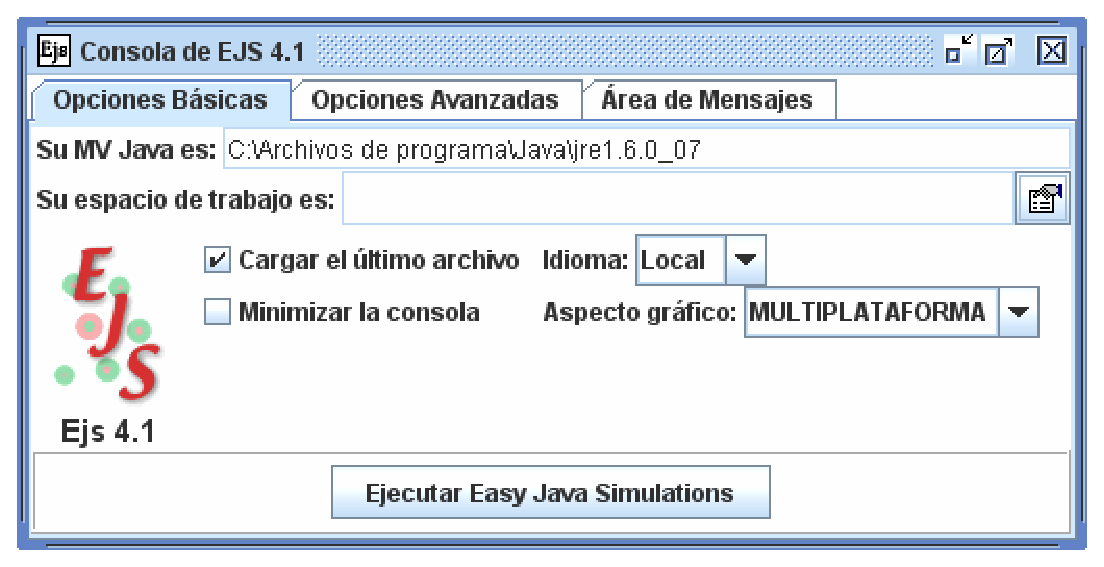
\includegraphics[scale=\scale]{02EjsIntro/images/EjsConsole1.eps}}
%  \subfigure[Console's output area.]{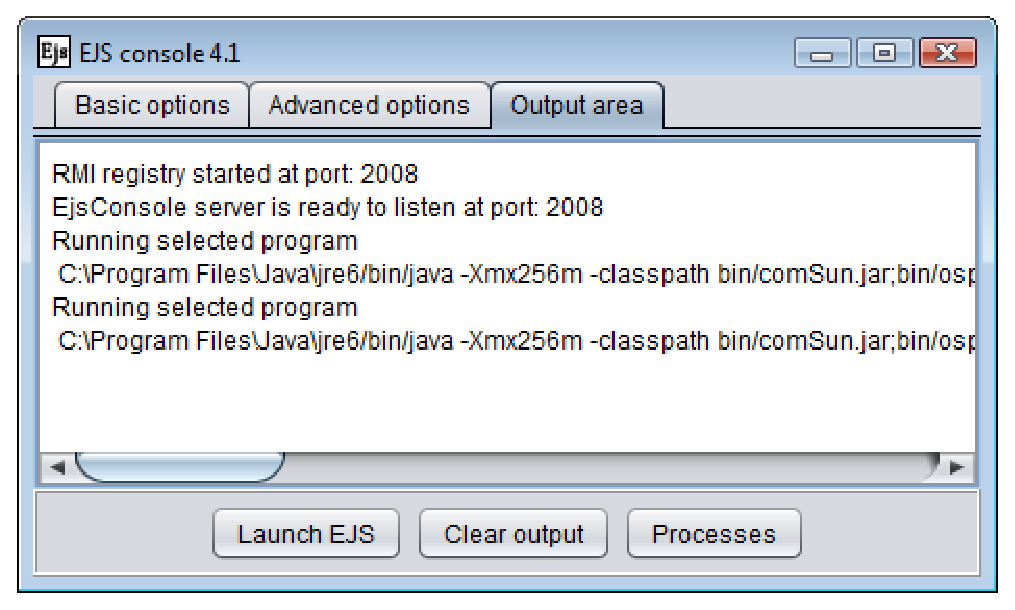
\includegraphics[scale=\scale]{02EjsIntro/images/EjsConsole2.eps}}
%  \caption{Two views of the \ejs\ console.}
  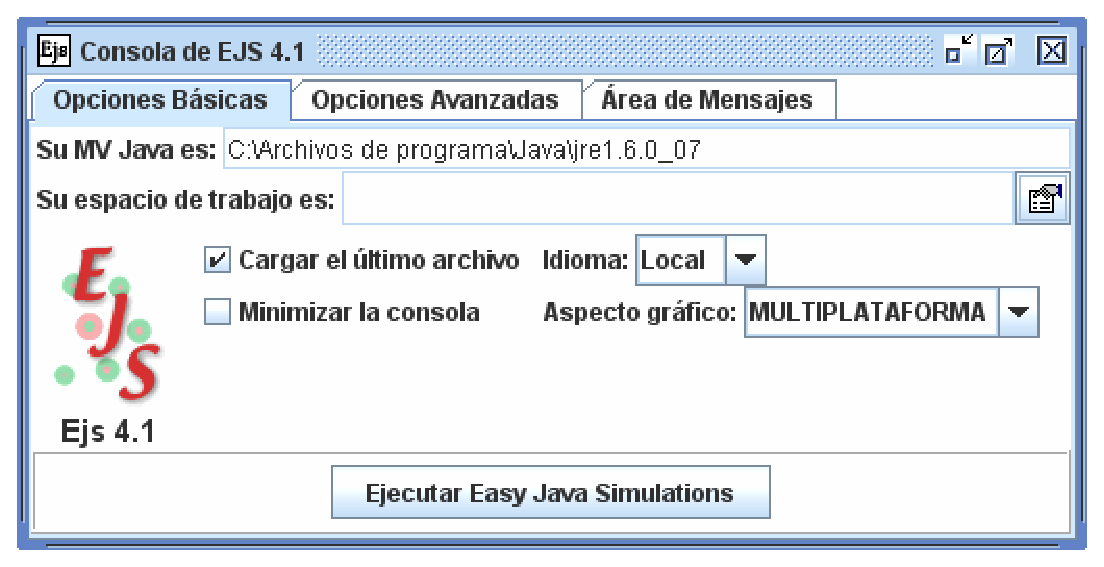
\includegraphics[scale=\scale]{02EjsIntro/images/EjsConsole1.eps}
  \caption{Consola de \ejs.}
  \label{fig:02EjsIntro/EjsConsole}
\end{figure}

\end{numberlist}

La consola deber�a verse en su pantalla como en la Figura~\ref{fig:02EjsIntro/EjsConsole}. Esta consola no es parte de \ejs, sino una utilidad usada para lanzar una o varias copias de \ejs\ y llevar a cabo otras tareas relacionadas con \ejs. La consola muestra por pantalla informaci�n del programa y mensajes de error y nos referiremos a ella en alguna que otra ocasi�n a lo largo de este libro. La consola crea una instancia (copia) de \ejs\ al inicio y termina autom�ticamente cuando se cierra la �ltima instancia de \ejs\ en funcionamiento. Otras propiedades de la consola, como su capacidad de procesar colecciones de modelos \ejs, se describen en los ap�ndices.

Sin embargo, antes de  que la consola de \ejs\ se ejecute tras la instalaci�n, aparecer� la ventana que puede ver en la Figura~\ref{fig:02EjsIntro/WorkspaceChooser}, donde se le pedir� elegir el directorio de su disco duro que servir� de \emph{espacio de trabajo}.

\begin{figure}[htb]
  \centering
  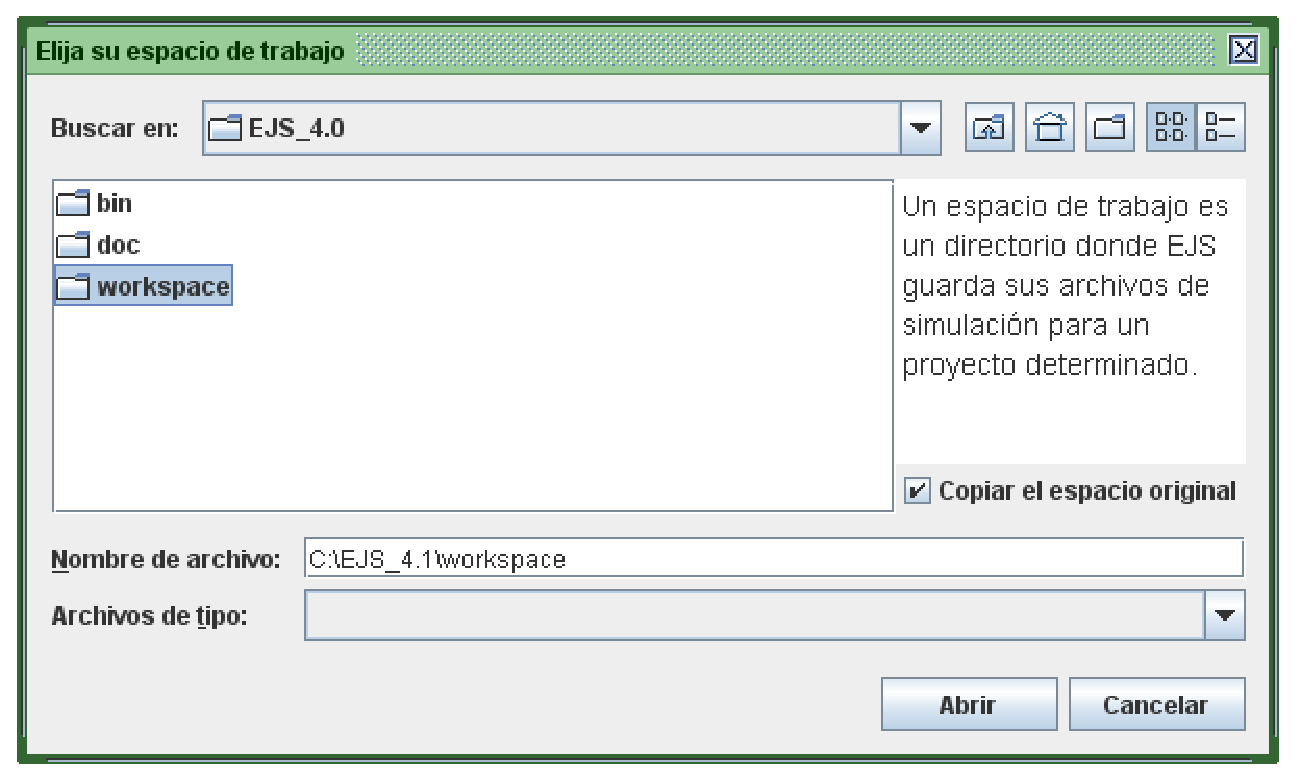
\includegraphics[scale=\scale]{02EjsIntro/images/WorkspaceChooser.eps}
  \caption{Elecci�n del directorio para el Espacio de Trabajo.}
  \label{fig:02EjsIntro/WorkspaceChooser}
\end{figure}

\ejs\ utiliza el concepto de espacio de trabajo para organizar su trabajo. El espacio de trabajo es un directorio en su disco duro donde \ejs\ almacena los archvos de las simulaciones de un proyecto determinado, pudiendo almacenar un n�mero ilimitado de �stos. Dentro de un espacio de trabajo, \ejs\ crea cuatro subdirectorios:

\index{\Ejs!directory structure}
\begin{bulletlist}
  \item \file{config} es el directorio donde \ejs\ guarda la configuraci�n determinada por el usuario y otros archivos de opciones.
  \item \file{export} es el directorio de destino propuesto por \ejs\ cuando se generan archivos listos para su distribuci�n.
  \item \file{output} es el directorio usado por \ejs\ para situar los archivos temporales generados cuando compilamos una simulaci�n.
  \item \file{source} es el directorio donde debe usted colocar todos los archivos necesarios para sus simulaciones (tanto los fuente como los auxiliares).
\end{bulletlist}

La primera vez que se ejecuta \ejs, la consola nos pide que elijamos un directorio para nuestro espacio de trabajo. �ste debe ser un directorio con permiso de escritura, situado en cualquier lugar de nuestro disco duro. Se puede elegir el espacio de trabajo incluido en la distribuci�n, es decir, el directorio \file{workspace} de la carpeta \file{EJS\_X.x} creada al descomprimir el paquete de \ejs. Aunque se recomienda crear una nueva carpeta en su directorio habitual destinada a ello. El cuadro de di�logo que le permite elegir el espacio de trabajo tiene una casilla que, si se marca, har� una copia de los archivos de ejemplo que contiene la distribuci�n en el nuevo espacio de trabajo. Deje la casilla marcada y encontrar� algunos subdirectorios en el directorio \file{source} de su espacio de trabajo que contienen simulaciones de muestra. En particular, el directorio \file{ModelizandoLaCiencia} incluye los modelos de \ejs\ de los que se habla en este libro.

\note{Se puede crear m�s de un espacio de trabajo para diferentes proyectos o tareas. La consola contiene un selector que permite cambiar el espacio de trabajo en uso y \ejs\ recordar� el actual espacio de trabajo de una sesi�n a otra o incluso si se reinstala el programa. En el Ap�ndice~\ref{appendix:Distribution} se describe c�mo configurar y usar \ejs\ en una instalaci�n para m�s de un usuario.}

Finalmente, tambi�n la primera vez que ejecute \ejs, el programa le solicitar� que introduzca su nombre y filiaci�n. Este paso es opcional aunque recomendado, ya que le ayudar� a documentar sus futuras simulaciones. Puede usted introducir o modificar esta informaci�n posteriormente a trav�s del icono de opciones de la barra de tareas de \ejs.

Ahora ya estamos preparados para centrar nuestra atenci�n en la herramienta de modelado \ejs, que se muestra en la Figura~\ref{fig:02EjsIntro/EjsInterface} con algunas anotaciones. A pesar de presentar una interfaz sencilla, \ejs\ contiene todas las herramientas necesarias para el ciclo completo de modelizaci�n.

\begin{figure}[htb]
  \centering
  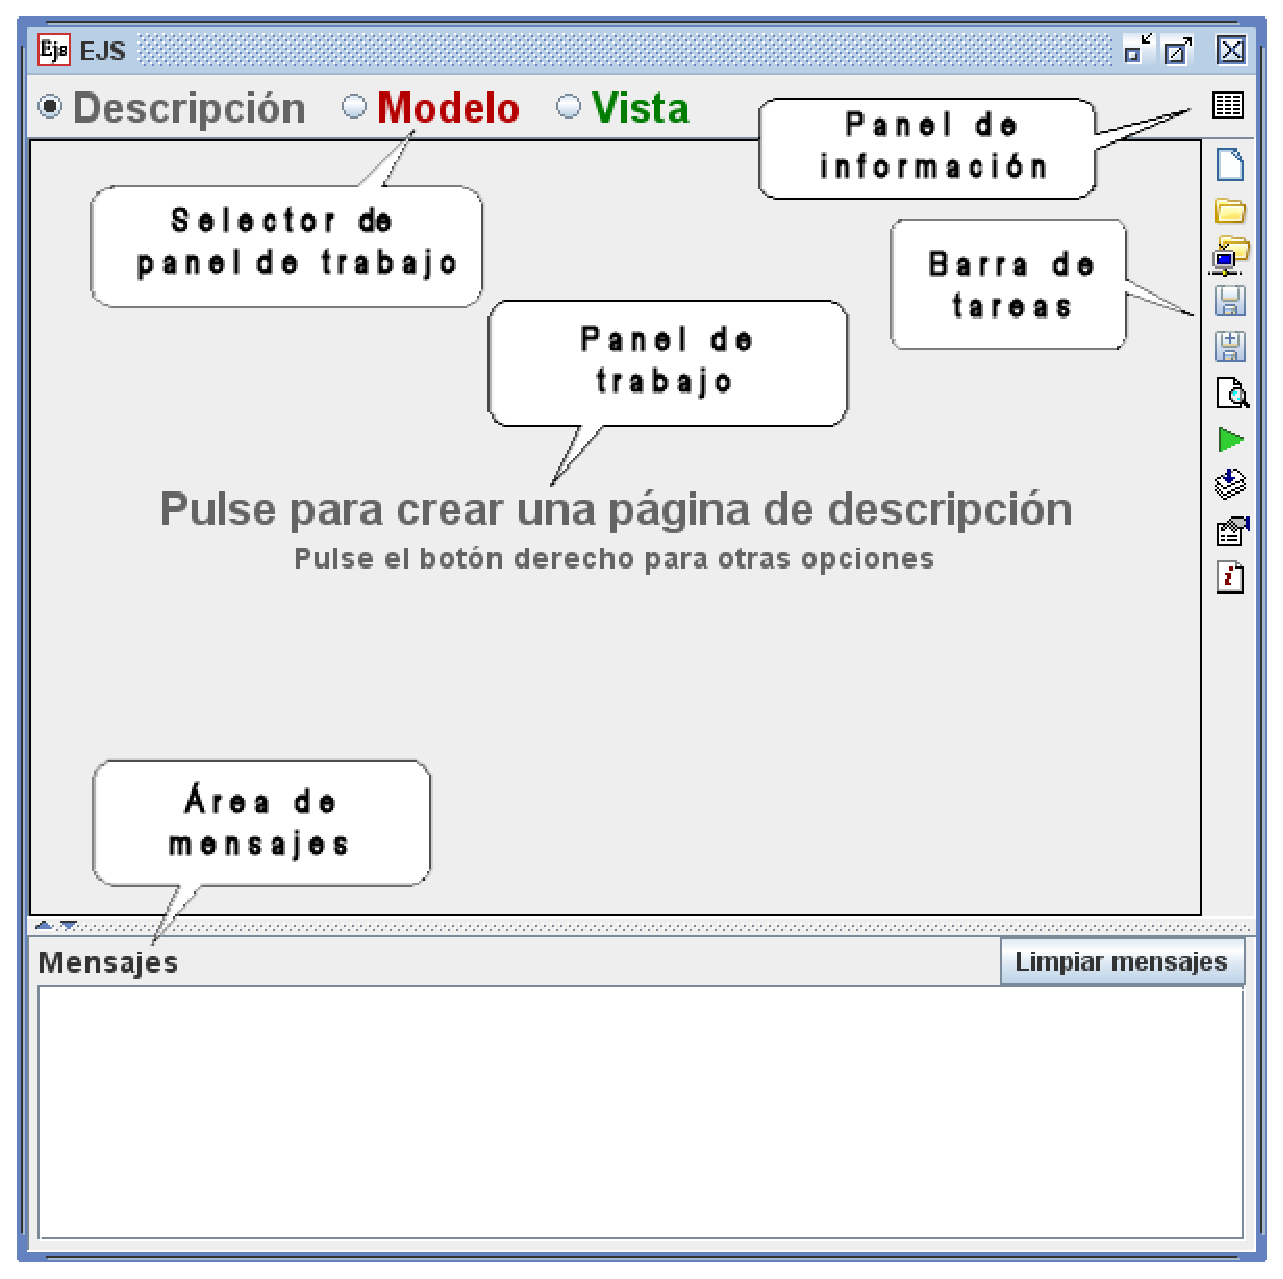
\includegraphics[scale=\scale]{02EjsIntro/images/EjsInterface.eps}
  \caption{Interfaz de \Ejs\ con anotaciones.}
  \label{fig:02EjsIntro/EjsInterface}
\end{figure}

La barra de tareas \index{\Ejs!taskbar} de la derecha muestra una serie de iconos para crear, abrir, buscar en y guardar un archivo, configurar \ejs, mostrar informaci�n sobre el programa y ayuda. Adem�s, posee iconos para ejecutar una simulaci�n y para almacenar una o m�s simulaciones en un solo archivo comprimido de tipo jar. Haciendo clic con el bot�n derecho de su rat�n sobre los iconos de la barra de tareas podr� elegir otras acciones alternativas relacionadas que iremos describiendo conforme vayan siendo necesarias. La parte inferior de la interfaz  contiene un �rea de mensajes\index{\Ejs!output area} donde \ejs\ nos muestra informaci�n. La parte central de la interfaz contiene los paneles de trabajo donde se construye la simulaci�n.

\Ejs\ contiene tres paneles de trabajo. El primer panel, llamado \lit{Descripci�n}, nos permite crear un documento multimedia en HTML que describa nuestro modelo.\index{HTML} Cada p�gina aparece en una pesta�a dentro del panel y, haciendo clic con el bot�n derecho del rat�n sobre la pesta�a, el usuario podr� editar la p�gina o importar otras existentes. El segundo panel, \lit{Modelo}, est� dedicado al proceso de modelado. Usaremos este panel para crear variables que describan el modelo, para inicializar dichas variables y para escribir algoritmos que describan c�mo nuestro modelo cambia con el tiempo. El tercer panel, \lit{Vista}, est� dedicado a la tarea de construir la interfaz gr�fica para el usuario final que permitir� controlar la simulaci�n y mostrar sus salidas. Construiremos la interfaz eligiendo elementos de las distintas paletas y a�adi�ndolos a la vista del \lit{�rbol de elementos}. Por ejemplo, la paleta de \lit{Interfaz} contiene botones, barras de desplazamiento y campos de texto, y la paleta de \lit{Elementos de dibujo 2D} contiene elementos para trazar datos en dos dimensiones.

% ------------------------
    \section{Inspeccionando la Simulaci�n}\label{section:02Inspecting}\index{\Ejs!inspecting a simulation}
% ------------------------

Para entender c�mo los paneles de trabajo, \lit{Descripci�n}, \lit{Modelo} y \lit{Vista}, funcionan coordinadamente, vamos a inspeccionar y ejecutar una simulaci�n ya existente.  Las salidas por pantalla no pueden sustituir a una demostraci�n en vivo por lo que le animamos a que realice las acciones en su ordenador conforme avance en la lectura.

\begin{figure}[htb]
  \centering
  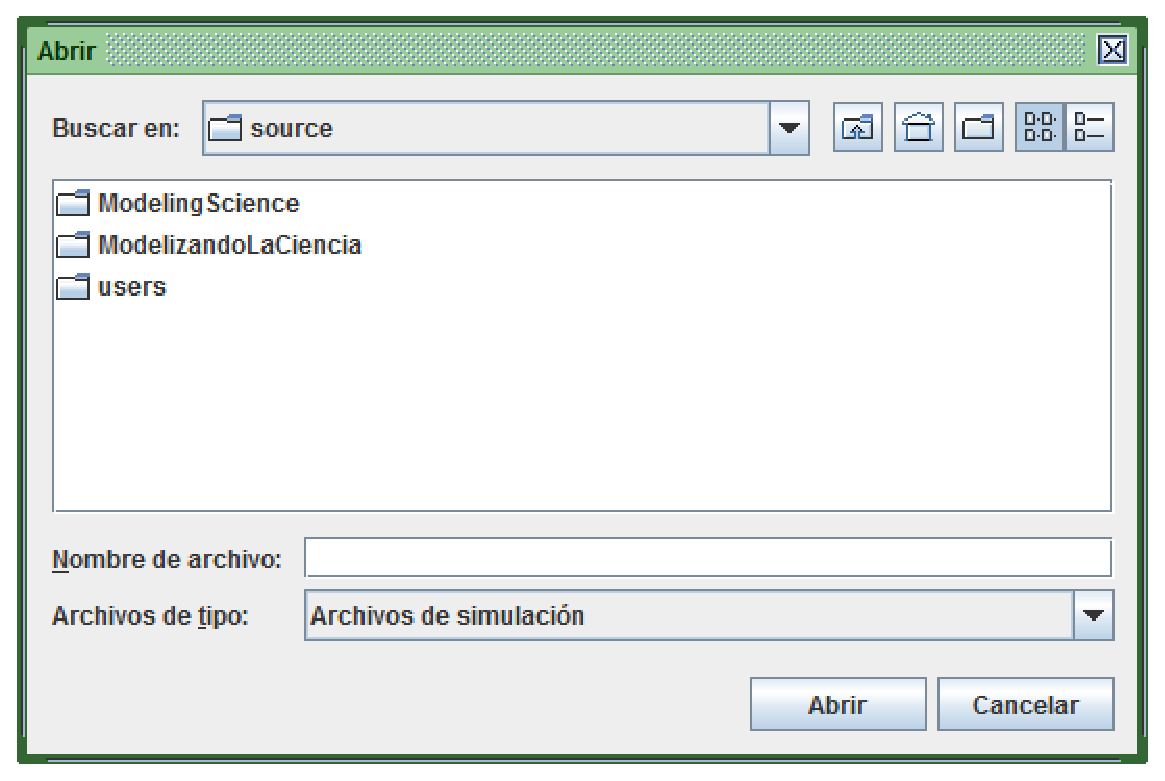
\includegraphics[scale=\scale]{02EjsIntro/images/OpenDialog.eps}
  \caption{El cuadro de di�logo \lit{Abrir} le permite buscar en su disco duro y cargar simulaciones existentes.}
  \label{fig:02EjsIntro/OpenDialog}
\end{figure}

Haga clic en el icono \lit{Abrir} 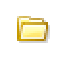
\includegraphics[scale=\linescale]{images/openSmall.eps} en la barra de tareas de \ejs\ y aparecer� un cuadro de di�logo parecido al que se muestra en la Figura~\ref{fig:02EjsIntro/OpenDialog} mostr�ndonos el contenido del directorio \file{source} de su espacio de trabajo. Vaya al directorio \file{ModelizandoLaCiencia} y abra el subdirectorio \file{Cap02\_Intro} all� encontrar� un archivo llamado \file{MasaYMuelle.xml}. Seleccione este archivo y haga clic en el bot�n \lit{Abrir} de la ventana.

�Ahora las cosas cobran vida! \ejs\ lee el documento \file{MasaYMuelle.xml} a partir de cuyo contenido rellena los paneles de trabajo y aparecen dos nuevas ventanas de \ejs\ en su pantalla, como muestra la Figura~\ref{fig:02EjsIntro/SpringInterface}. Una advertencia: Los objetos pueden ser arrastrados sobre la ventana de la maqueta pero esto determinar� las condiciones iniciales. Normalmente es mejor determinar las condiciones elementales utilizando la tabla de variables que se describe en la Secci�n~\ref{section:02Model}.


\begin{figure}[htb]
  \centering
  \subfigure{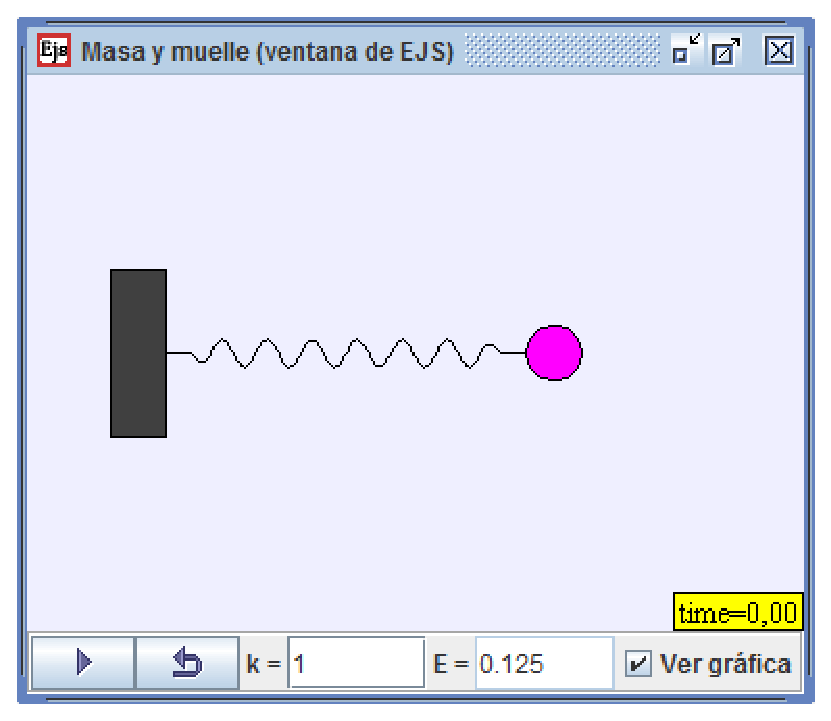
\includegraphics[scale=\scale]{02EjsIntro/images/SpringInterface1.eps}}
  \subfigure{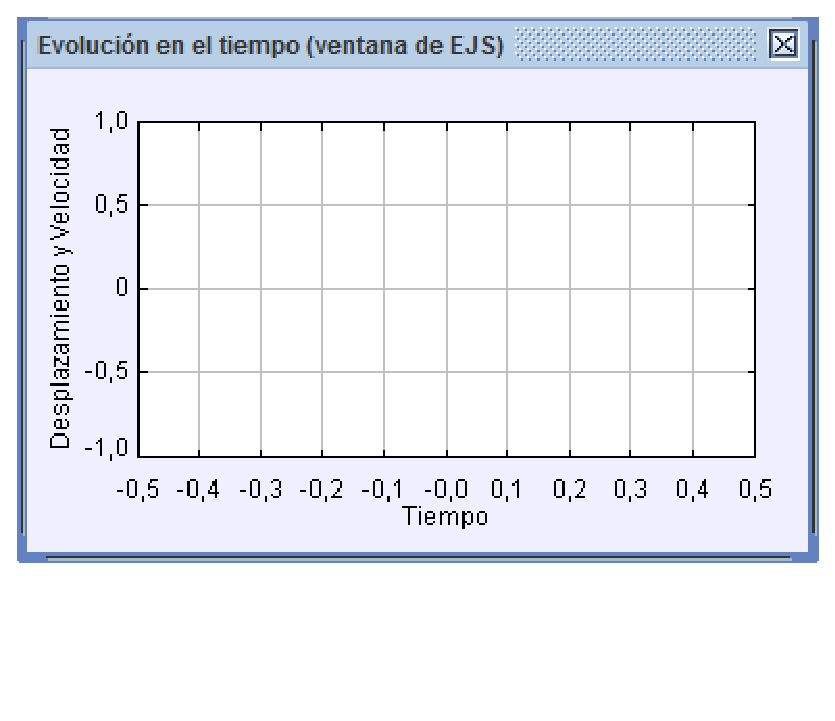
\includegraphics[scale=\scale]{02EjsIntro/images/SpringInterface2.eps}}
  \caption{Ventana de la maqueta de \ejs\ para la simulaci�n \file{Masa y Muelle}. El t�tulo de la ventana muestra que son ventanas de \ejs\ y que el programa no est� ejecut�ndose.}
  \label{fig:02EjsIntro/SpringInterface}
\end{figure}

\note{Los lectores m�s impacientes o precoces puede que hayan intentado hacer clic sobre el bot�n verde de ejecuci�n 
\includegraphics[scale=\linescale]{images/launch.eps} de la barra de tareas para ejecutar nuestro ejemplo antes de continuar con este tutorial. Aquellos lectores que hayan hecho esto no estar�n interactuando con \ejs\ sino con un programa Java compilado y ejecutado. Salga de la ejecuci�n del programa cerrando la ventana \lit{Masa y muelle} o haciendo clic con el bot�n derecho en el bot�n de ejecuci�n 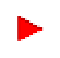
\includegraphics[scale=\linescale]{images/launchRed.eps}(ahora en color rojo) antes de continuar.}

\subsection{El panel de la \lit{Descripci�n}}

Seleccione el panel de \lit{Descripci�n}\index{Ejs!Description} haciendo clic sobre el selector en la parte superior de la ventana de \ejs\ y podr� ver dos p�ginas de narraci�n sobre esta simulaci�n. La primera p�gina, que se muestra en la Figura~\ref{fig:02EjsIntro/SpringDesc}, contiene una breve explicaci�n sobre el modelo de masa y muelle. Haga clic en la pesta�a \lit{Actividades} para ver la segunda p�gina.

\begin{figure}[htb]
  \centering
  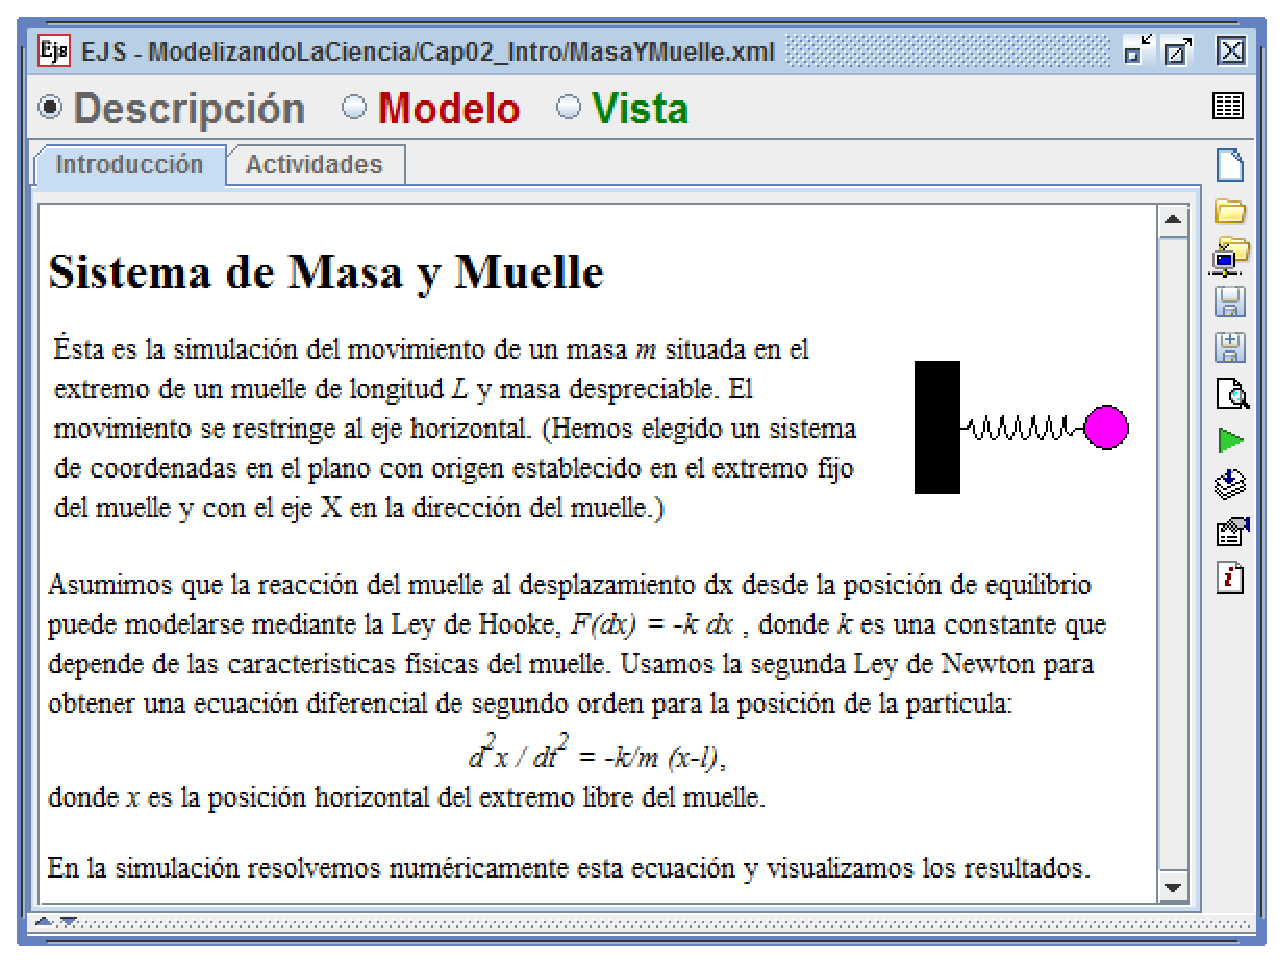
\includegraphics[scale=\scale]{02EjsIntro/images/SpringDesc.eps}
  \caption{P�ginas de descripci�n para la simulaci�n de la masa y el muelle. Haga clic en una pesta�a para mostrar la p�gina correspondiente. Haga clic con el bot�n derecho para editarla.}
  \label{fig:02EjsIntro/SpringDesc}
\end{figure}

Una \lit{Descripci�n} es un texto multimedia en formato HTML\index{HTML} que proporciona informaci�n e instrucciones sobre la simulaci�n. HTML significa Lenguaje de Marcas de Hipertexto (HyperText Markup Language) y es el protocolo m�s usado para dar formato a los documentos de las p�ginas Web. \ejs\ proporciona un sencillo editor de HTML que permite crear y modificar p�ginas desde \ejs. Tambi�n se pueden importar p�ginas haciendo clic con el bot�n derecho sobre una de las pesta�as del panel de trabajo (Ver Secci�n~\ref{section:02ModifyingDescription}.) Las p�ginas de descripci�n son una parte esencial del proceso de modelado y estas p�ginas se distribuyen junto con el modelo compilado cuando el modelo es distribuido como una aplicaci�n Java o  publicado en un servidor Web como un subprograma (applet). Estas opciones de distribuci�n se describen en el Ap�ndice ~\ref{appendix:Distribution}.

\subsection{El panel del \lit{Modelo}}\label{section:02Model}

El panel de trabajo \lit{Modelo} es donde se define el modelo de modo que pueda ser convertido en un programa por \ejs. En esta simulaci�n, estudiaremos el movimiento de una part�cula de masa $m$ unida a uno de los extremos de un muelle de masa despreciable y de longitud en equilibrio $L$. El muelle est� unido a una pared por su otro extremo y se mueve estrictamente en horizontal. Aunque la masa oscilante tiene una soluci�n anal�tica bien conocida, es �til empezar con un modelo del oscilador arm�nico simple con el fin de poder comparar nuestra soluci�n num�rica con el resultado anal�tico exacto.\index{Simple Harmonic Motion}

Nuestro modelo asume que se producen �nicamente oscilaciones peque�as, de modo que el muelle responde a un desplazamiento (horizontal), $\delta x$, desde su posici�n de equilibrio, $L$, con una fuerza dada por la ley de Hooke,\index{Hooke's law} $F_x = - k \,\delta x$, donde $k$ es la constante de elasticidad del muelle que depende de las caracter�sticas f�sicas del mismo. Usamos la segunda ley de Newton\index{Newton's second law} para obtener una ecuaci�n diferencial de segundo orden  para la posici�n de la part�cula:

\begin{equation}
  \frac{d^2\ x}{dt^2} = -\frac{k}{m}\,(x-L). \label{eq:02EjsIntro/SpringBasic}
\end{equation}
Observe que usamos un sistema de coordenadas con el eje X situado a lo largo del muelle y con origen en el extremo fijo del muelle. La part�cula se encuentra en la posici�n $x$ y su desplazamiento desde la posici�n de equilibrio, $\delta x=x-L$, es cero cuando $x=L$. Resolvemos este sistema num�ricamente para estudiar c�mo evoluciona el modelo con el paso del tiempo.

Vamos a examinar c�mo hemos implementado el modelo de masa y muelle eligiendo el selector \lit{Modelo} e inspeccionando cada uno de sus cinco paneles.

\subsubsection{Declaraci�n de variables}
\begin{figure}[htb]
    \centering
  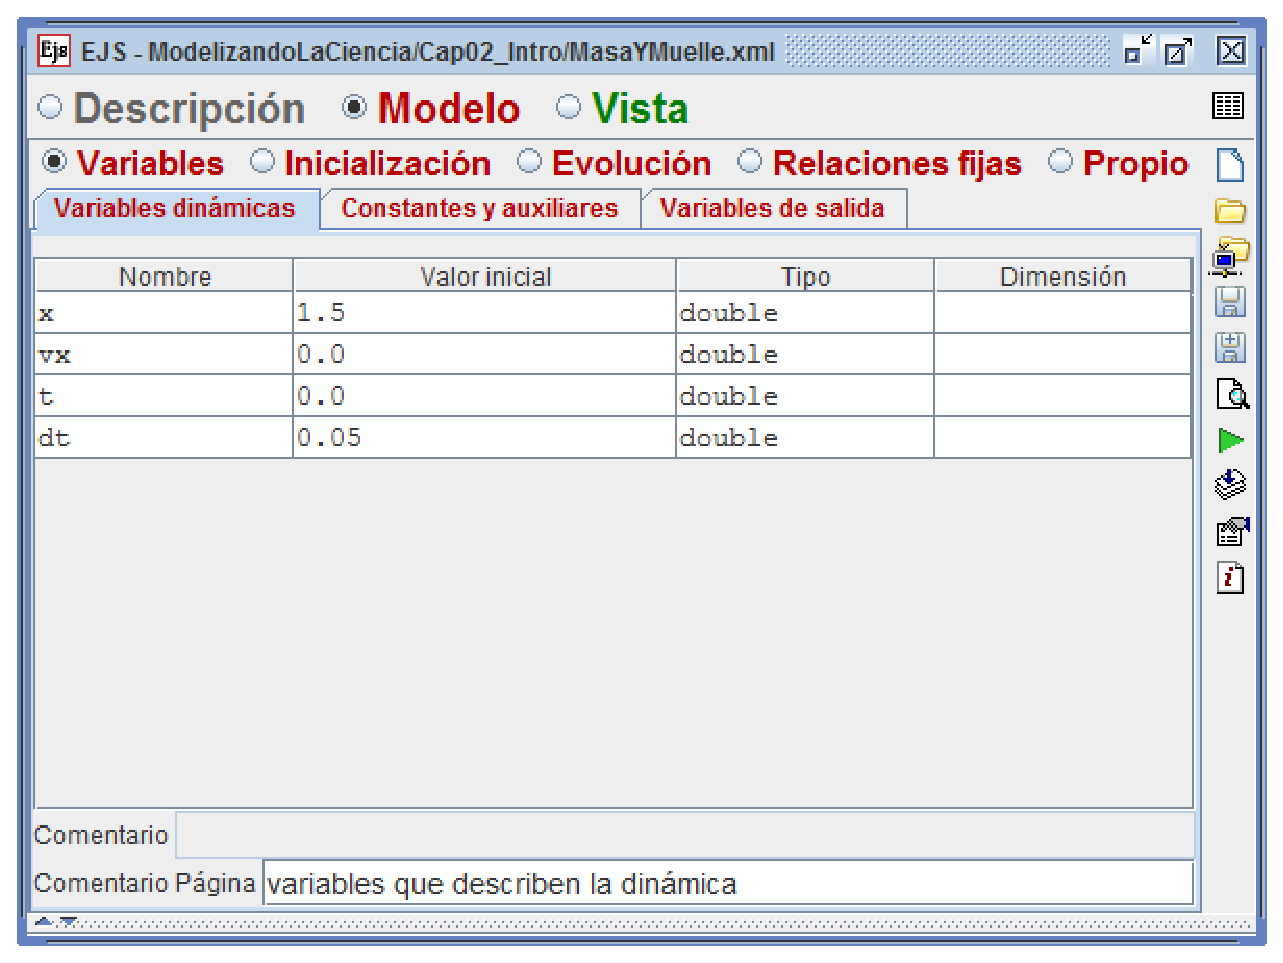
\includegraphics[scale=\scale]{02EjsIntro/images/ModelVariables.eps}
    \caption{El panel de trabajo \lit{Modelo} contiene cinco subpaneles. Se muestra el subpanel para la definici�n de las variables din�micas del ejemplo. Otras pesta�as en este subpanel definen variables adicionales tales como la longitud del muelle $L$ y la energ�a $E$.} \label{fig:02EjsIntro/ModelVariables}
\end{figure}

Cuando implementamos un modelo, un buen primer paso es identificar, definir e inicializar las variables que describen nuestro sistema. El t�rmino \emph{variable} es muy general y se refiere a cualquier cosa a la que podemos dar un nombre, incluyendo una constante f�sica o un gr�fico\index{Model!Variables}. La Figura~\ref{fig:02EjsIntro/ModelVariables} nos muestra una tabla de variables en \ejs. Cada fila define una variable del modelo especificando para ella un nombre, un tipo, una dimensi�n y un valor inicial.

Las variables en los programas de ordenador pueden ser de varios tipos dependiendo de la informaci�n que guardan. Los tipos m�s frecuente son \code{boolean} que se utiliza para los valores verdadero/falso, \code{int} para enteros, \code{double} para n�meros de alta precisi�n ($\approx 16$ d�gitos significativos) y \code{String} para textos. Usaremos los distintos tipos a lo largo del libro pero el modelo de masa y muelle s�lo utiliza  variables de tipo double y boolean.

Las variables pueden ser utilizadas como par�metros, \index{Model!Parameters} variables de estado,\index{Model!State variables} o para entradas y salidas del modelo.\index{Model!Input and Output} Nosotros hemos declarado una variable para el tiempo, \code{t}, otra para la posici�n de la part�cula, \code{x}, y otra para la velocidad en la direcci�n del eje X, \code{vx}. Adem�s hemos definido variables que no aparecen en \eqref{eq:02EjsIntro/SpringBasic}. La raz�n de estas variables auxiliares, como la energ�a cin�tica, la energ�a potencial y la energ�a total, se aclarar� m�s adelante. En la parte inferior del panel de variables encontramos un campo para comentarios que proporciona una descripci�n del papel de cada variable en el modelo. Haciendo clic en cada una de las variables podremos ver el comentario correspondiente.

\subsubsection{Inicializaci�n del modelo}
Establecer correctamente las condiciones iniciales del modelo es importante en su implementaci�n ya que el modelo ha de comenzar en una situaci�n f�sicamente posible. Nuestro modelo es relativamente simple y lo inicializamos  con valores enteros (o expresiones simples en Java como \code{0.5*m*vx*vx}) en la columna \lit{Valor inicial} de la tabla de variables y \ejs\ utiliza dichos valores cuando se inicia la simulaci�n.

\note{Modelos m�s avanzados pueden requerir un algoritmo de inicializaci�n. Por ejemplo, un modelo molecular din�mico debe establecer las velocidades de un conjunto de part�culas. El panel de \lit{Inicializaci�n} nos permite definir una o m�s p�ginas de c�digo Java que realicen el c�lculo necesario. \ejs\ convierte este c�digo en un m�todo Java\index{Java!method}\footnote{Un m�todo Java es algo parecido a una funci�n o una subrutina en lenguajes de programaci�n procedimental.} y llama a este m�todo al empezar y siempre que la simulaci�n sea reiniciada. El panel de la \lit{Inicializaci�n} del modelo de masa y muelle no se muestra aqu� porque est� vac�o. Vaya a la Secci�n~\ref{section:02InspectingRelations} para ver un ejemplo de c�mo aparece en \ejs\ el c�digo Java.}

\subsubsection{La evoluci�n del modelo}

El panel de \lit{Evoluci�n} nos permite escribir c�digo Java que determine c�mo el sistema masa-muelle se desarrolla en el tiempo y usaremos esta opci�n frecuentemente para modelos no basados en ecuaciones diferenciales ordinarias (EDOs). Hay sin embargo una segunda opci�n que nos permite introducir ecuaciones diferenciales ordinarias, como \eqref{eq:02EjsIntro/SpringBasic}, sin utilizar programaci�n. \ejs\ proporciona un editor dedicado a esta tarea que nos permite especificar ecuaciones diferenciales en un formato que utiliza la notaci�n matem�tica y que genera autom�ticamente el c�digo Java necesario.

Veamos c�mo el editor de ecuaciones diferenciales funciona para nuestro modelo de masa y muelle. Como los algoritmos de resoluci�n de EDO resuelven sistemas de primer orden, una ecuaci�n de orden superior, como \eqref{eq:02EjsIntro/SpringBasic}, debe ser reducida a un sistema de primer orden. Conseguimos �sto estableciendo la velocidad como una variable independiente que obedece a su propia ecuaci�n:
\begin{align}
  \frac{d\ x} {dt} &= v_x                  \label{eq:02EjsIntro/SpringBasicODE1} \\
  \frac{d\ v_x}{dt} &= -\frac{k}{m}\,(x-L). \label{eq:02EjsIntro/SpringBasicODE2}
\end{align}
La necesidad de una ecuaci�n diferencial adicional explica por qu� hab�amos declarado la variable \code{vx} en nuestra tabla de variables

Haciendo clic en el panel de \lit{Evoluci�n} se muestra el editor de EDO que aparece en la Figura~\ref{fig:02EjsIntro/ModelEvolution}.

\begin{figure}[htb]
    \centering
  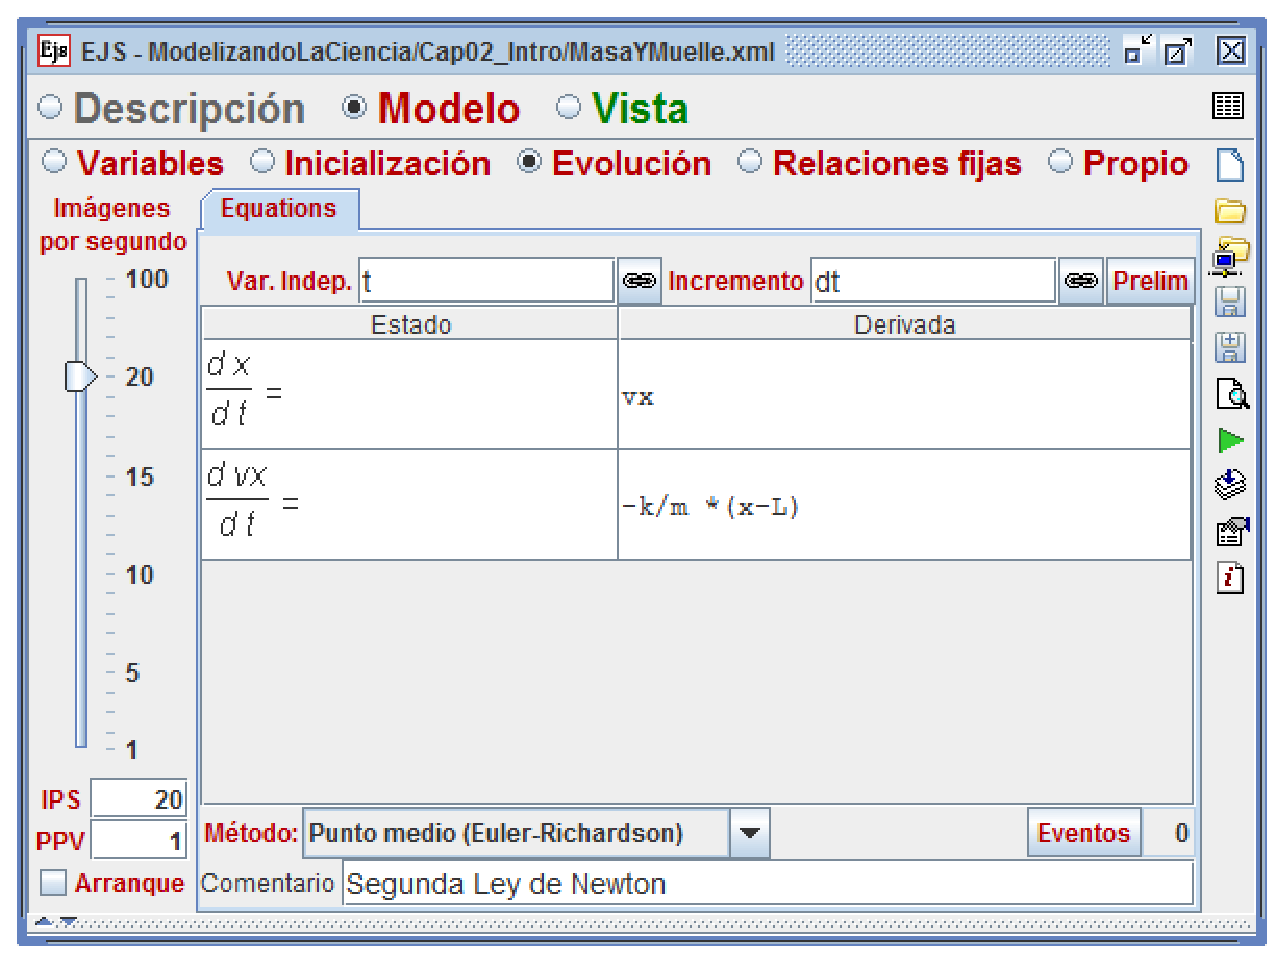
\includegraphics[scale=\scale]{02EjsIntro/images/ModelEvolution.eps}
    \caption{El panel de evoluci�n de EDO mostrando la ecuaci�n diferencial del modelo de masa y muelle y el algoritmo num�rico.}
    \label{fig:02EjsIntro/ModelEvolution}
\end{figure}

 N�tese que el editor de EDO  muestra las ecuaciones \eqref{eq:02EjsIntro/SpringBasicODE1} y \eqref{eq:02EjsIntro/SpringBasicODE2} (usando el s�mbolo \lit{*} para denotar la multiplicaci�n). Los campos en la parte superior del editor especifican la variable independiente \code{t} y la variable incremento \code{dt}. Los algoritmos num�ricos aproximan la soluci�n exacta a la ecuaci�n avanzando el estado en pasos discretos donde el incremento determina el tama�o del paso. El bot�n \lit{Prelim} en la parte superior derecha del editor nos permite introducir un c�digo preliminar que se encargue de los c�lculos previos a la evaluaci�n de las ecuaciones (circunstancia que se precisa en situaciones m�s complejas que la que tratamos en este ejemplo).
Un men� desplegable en la parte inferior del editor nos permite seleccionar el algoritmo num�rico de resoluci�n de EDOs a emplear, el cual avanza la soluci�n desde el valor actual para el tiempo, \code{t}, al siguiente valor, \code{t + dt}. El campo de eventos de la parte inferior del panel nos dice que no hemos definido ning�n evento para esta ecuaci�n diferencial. Podemos encontrar ejemplos con c�digo preliminar y eventos en el Cap�tulo~\ref{chapter:Events}.

La parte izquierda del panel de trabajo \lit{Evoluci�n} incluye campos para determinar c�mo de suave y r�pidamente queremos que funcione la simulaci�n. El n�mero de \lit{im�genes por segundo} (\lit{IPS}) especifica cu�ntas veces por segundo queremos que nuestra simulaci�n sea repintada en la pantalla. El n�mero de \lit{pasos por visualizaci�n} (\lit{PPV}) especifica cu�ntas veces (pasos) queremos que avance el modelo antes de repintar. El valor actual de \code{20} im�genes por segundo produce una animaci�n fluida que, junto con el valor por defecto de un paso por visualizaci�n y el valor de \code{0.05} para \code{dt}, resulta en una simulaci�n que funciona (aproximadamente) en tiempo real. Nosotros utilizaremos casi siempre la elecci�n por defecto de un paso por visualizaci�n. Sin embargo, hay situaciones donde la salida gr�fica del modelo consume una cantidad significativa de capacidad de proceso y necesitaremos acelerar los c�lculos num�ricos. En este caso incrementaremos el n�mero de pasos por visualizaci�n de forma que el modelo avance varias veces antes de que se vuelva a dibujar la visualizaci�n. La casilla de \lit{Arranque} indica si la simulaci�n debe ponerse en marcha cuando el programa comience. En este caso, la casilla no est� marcada as� que podremos cambiar las condiciones iniciales antes de que empiece la evoluci�n.

El panel de \lit{Evoluci�n} maneja los aspectos t�cnicos del modelo de masa y muelle sin necesidad de programar. La simulaci�n avanza el estado del sistema en el tiempo mediante m�todos num�ricos de resoluci�n de ecuaciones diferenciales utilizando el algoritmo del punto medio. El algoritmo pasa del estado actual en el momento \code{t} a un nuevo estado en un nuevo momento \code{t + dt} antes de que la visualizaci�n se redibuje. La simulaci�n repite esta evoluci�n \code{20} veces cada segundo en ordenadores de una capacidad de procesamiento modesta. La simulaci�n podr�a fluir m�s lenta y no tan suave en ordenadores con una capacidad insuficiente o si el ordenador est� ocupado en otra tarea, pero no suele fallar.
\note{El modelo de masa y muelle puede resolverse con un simple algoritmo para EDOs. Nuestra librer�a de m�todos num�ricos contiene algoritmos mucho m�s sofisticados y \ejs\ puede aplicar dichos algoritmos a sistemas grandes con ecuaciones diferenciales vectoriales con o sin puntos de discontinuidad.}

\subsubsection{Relaciones entre variables}\label{section:02InspectingRelations}

No todas las variables del modelo se calculan utilizando algoritmos del panel de Evoluci�n. Algunas variables pueden ser tambi�n calculadas despu�s de que la evoluci�n se haya aplicado. Nos referiremos a las variables que se calculan utilizando el algoritmo de evoluci�n como variables de estado o variables din�micas, y nos referiremos a las variables que dependen de esas variables como variables auxiliares o de salida. En nuestro modelo la energ�a cin�tica, potencial y la energ�a total del sistema son variables de salida porque se calculan a partir de las variables de estado.
\begin{align}
  T &= \frac{1}{2} m {v_x}^2,     \label{eq:02EjsIntro/SpringEnergy1} \\
  V &= \frac{1}{2} k (x-L)^2,     \label{eq:02EjsIntro/SpringEnergy2} \\
  E &= T + V.                     \label{eq:02EjsIntro/SpringEnergy3}
\end{align}

Decimos entonces que existen \emph{relaciones fijas} entre las variables del modelo.
El panel de \lit{Relaciones fijas}, mostrado en la Figura~\ref{fig:02EjsIntro/ModelRelations}, se usa para escribir las relaciones entre variables. N�tese qu� f�cil es convertir \eqref{eq:02EjsIntro/SpringEnergy1} a \eqref{eq:02EjsIntro/SpringEnergy3} a la sintaxis de Java. Aseg�rese siempre de utilizar el s�mbolo \lit{*} para la multiplicaci�n y de escribir un punto y coma al final de cada sentencia.

\begin{figure}[htb]
    \centering
  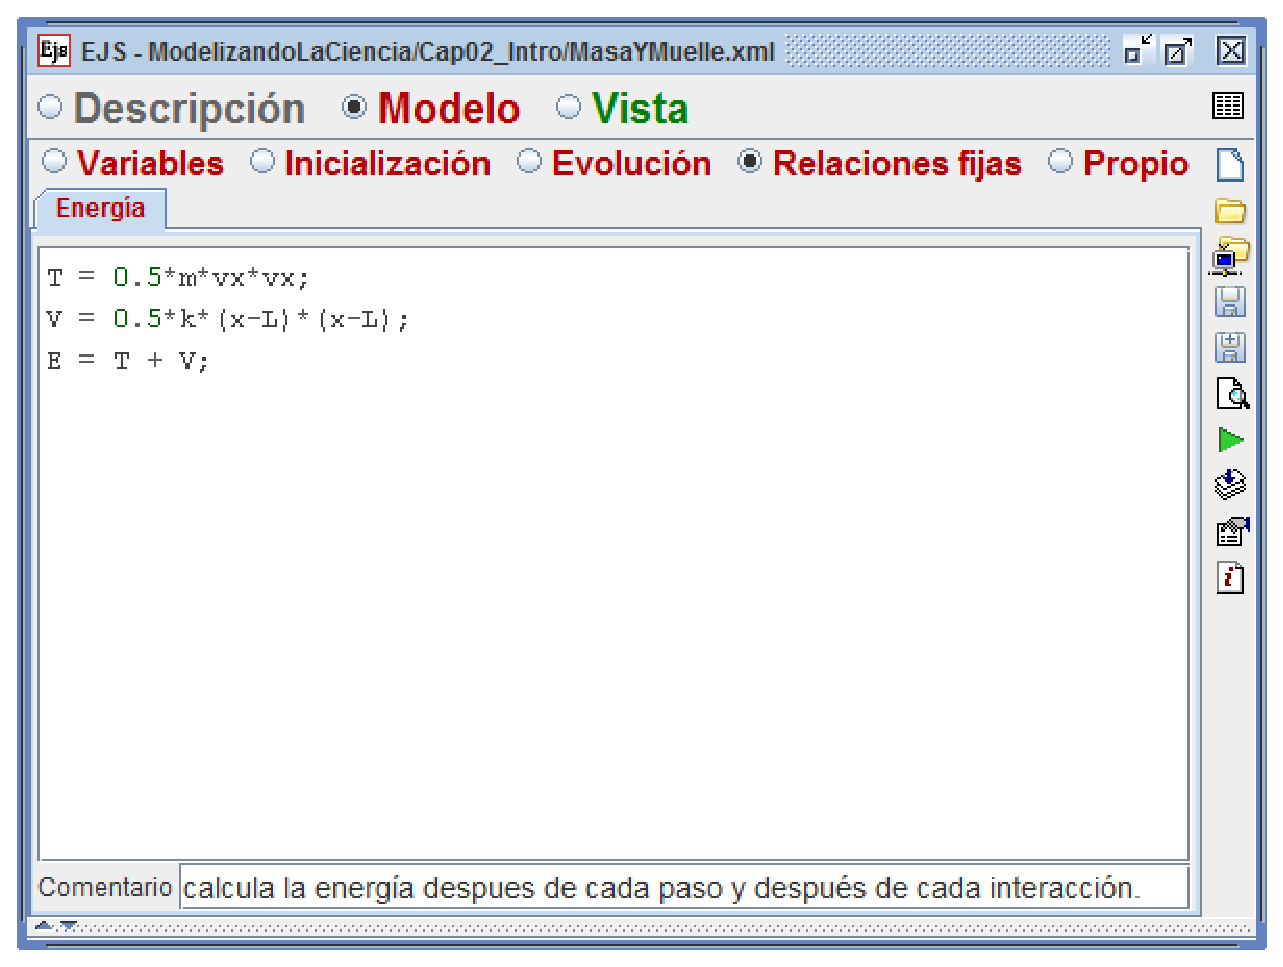
\includegraphics[scale=\scale]{02EjsIntro/images/ModelConstraints.eps}
    \caption{Relaciones fijas en el modelo de masa y muelle.}
    \label{fig:02EjsIntro/ModelRelations}
\end{figure}

Puede que se pregunte por qu� no escribimos las expresiones correspondientes a relaciones fijas a�adiendo una segunda p�gina de c�digo despu�s de la p�gina EDO en el panel de \lit{Evoluci�n}. Despu�s de todo las p�ginas de evoluci�n se ejecutan secuencialmente y una segunda p�gina podr�a actualizar correctamente la salida despu�s de cada paso. La raz�n de que no se use el panel de \lit{Evoluci�n} es que las relaciones deben mantenerse \emph{siempre} y hay acciones, como las hechas con el rat�n, que pueden afectar a las variables indicadas. Por ejemplo, arrastrando la masa cambiamos la variable $x$ y este cambio afecta a la energ�a. \ejs\ autom�ticamente eval�a las relaciones despu�s de la inicializaci�n, despu�s de cada paso y si hay alguna interacci�n del usuario con la interfaz de la simulaci�n. Por esta raz�n, es importante que las relaciones fijas se escriban en el panel destinado a ello.

\subsubsection{P�ginas \lit{Propio}}

En el panel de trabajo \lit{Modelo} hay un quinto panel llamado \lit{Propio}. Este panel puede usarse para definir m�todos Java (funciones) que pueden ser usadas a lo largo del modelo. Este panel est� vac�o porque el modelo actual no requiere m�todos adicionales, aunque haremos uso de este panel cuando modifiquemos nuestro ejemplo de masa y muelle en la Secci�n~\ref{section:02Modifying}. Un m�todo propio no se usa a menos que sea llamado expl�citamente desde otro panel de trabajo.


% ---------------------------------------------
\subsection{El panel de la \lit{Vista}}
% ---------------------------------------------

El tercer panel de trabajo de \Ejs\ es el panel de la \lit{Vista}. Este panel de trabajo permite crear una interfaz gr�fica que incluye la visualizaci�n, la interacci�n del usuario y el control del programa con una cantidad m�nima de programaci�n. La Figura~\ref{fig:02EjsIntro/SpringInterface} muestra la vista del modelo masa y muelle. Marque el selector \lit{Vista} para examinar c�mo ha sido creada la vista.

El marco de la derecha del panel de la vista, mostrado en la Figura~\ref{fig:02EjsIntro/View}, contiene una colecci�n de \emph{elementos para la vista}\index{Ejs!view elements} agrupados seg�n su funci�n. Los elementos para la vista funcionan como bloques de construcci�n que pueden ser combinados para formar una interfaz de usuario completa. Cada elemento para la vista es un objeto especializado con una representaci�n espec�fica en pantalla. Para ver informaci�n sobre un elemento, haga clic en su icono y presione la tecla \lit{F1} o haga clic con el bot�n derecho del rat�n y seleccione \lit{Ayuda} en el men� emergente que aparecer�. Para crear una interfaz de usuario creamos una ventana y a�adimos elementos, como botones y gr�ficos, con s�lo arrastrar y soltar, como se describe en la Secci�n~\ref{section:02Modifying}.

\begin{figure}[htb]
    \centering
  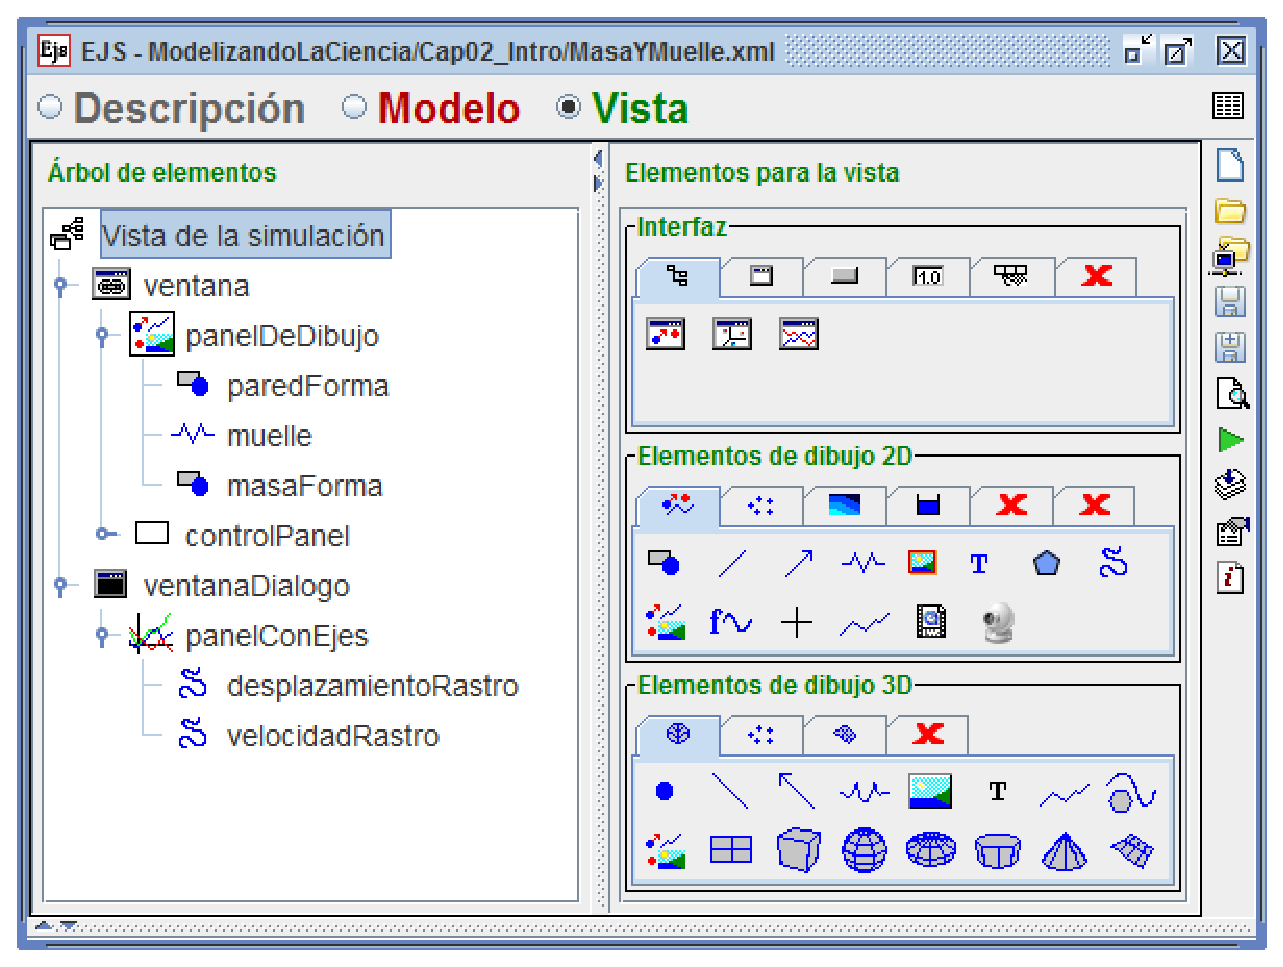
\includegraphics[scale=\scale]{02EjsIntro/images/View.eps}
    \caption{El panel de trabajo \lit{Vista} mostrando el \emph{�rbol de elementos} para la interfaz del modelo de masa y muelle.}
    \label{fig:02EjsIntro/View}
\end{figure}

El \emph{�rbol de elementos}, mostrado a la izquierda en la Figura~\ref{fig:02EjsIntro/View}, muestra la estructura de la interfaz del modelo de masa y muelle. N�tese que la simulaci�n tiene dos ventanas, una del tipo (\code{Ventana}) y otra del tipo (\code{VentanaDi�logo}), que aparecen en la pantalla de su ordenador. Estos elementos pertenecen al grupo de elementos \emph{contenedores}, cuyo principal cometido es organizar y agrupar visualmente otros elementos de la interfaz. El �rbol muestra nombres descriptivos e iconos para estos elementos. Haciendo clic con el bot�n derecho del rat�n en los elementos del �rbol aparece un men� que ayuda al usuario a modificar dicha estructura.

Cada elemento para la vista tiene un conjunto de par�metros internos llamados \emph{propiedades}\index{Ejs!view element properties} que configuran su apariencia y comportamiento. Podemos editar dichas propiedades haciendo doble clic en el elemento del �rbol para mostrar una tabla a la que llamamos \emph{inspector de propiedades}. A las propiedades de apariencia, como por ejemplo el color, se les asigna a menudo un valor constante, por ejemplo, \code{RED} (rojo, en ingl�s). Podemos tambi�n utilizar una variable del modelo para establecer el valor de una propiedad del elemento. Esta posibilidad de conectar una propiedad a una variable sin programar es la clave para obtener f�cilmente una visualizaci�n din�mica e interactiva.

Veamos c�mo se lleva a cabo este proceso en la pr�ctica. Haga doble clic en el elemento \code{masaForma} (el sufijo `Forma' que a�adimos al nombre de los elementos nos ayuda a reconocer el tipo del elemento) en el �rbol para mostrar su inspector de propiedades. Este elemento es la masa unida al lado que queda libre del muelle. La tabla de propiedades de este objeto aparece como se muestra en la Figura~\ref{fig:02EjsIntro/SpringBallProperties}.
\begin{figure}[htb]
    \centering
  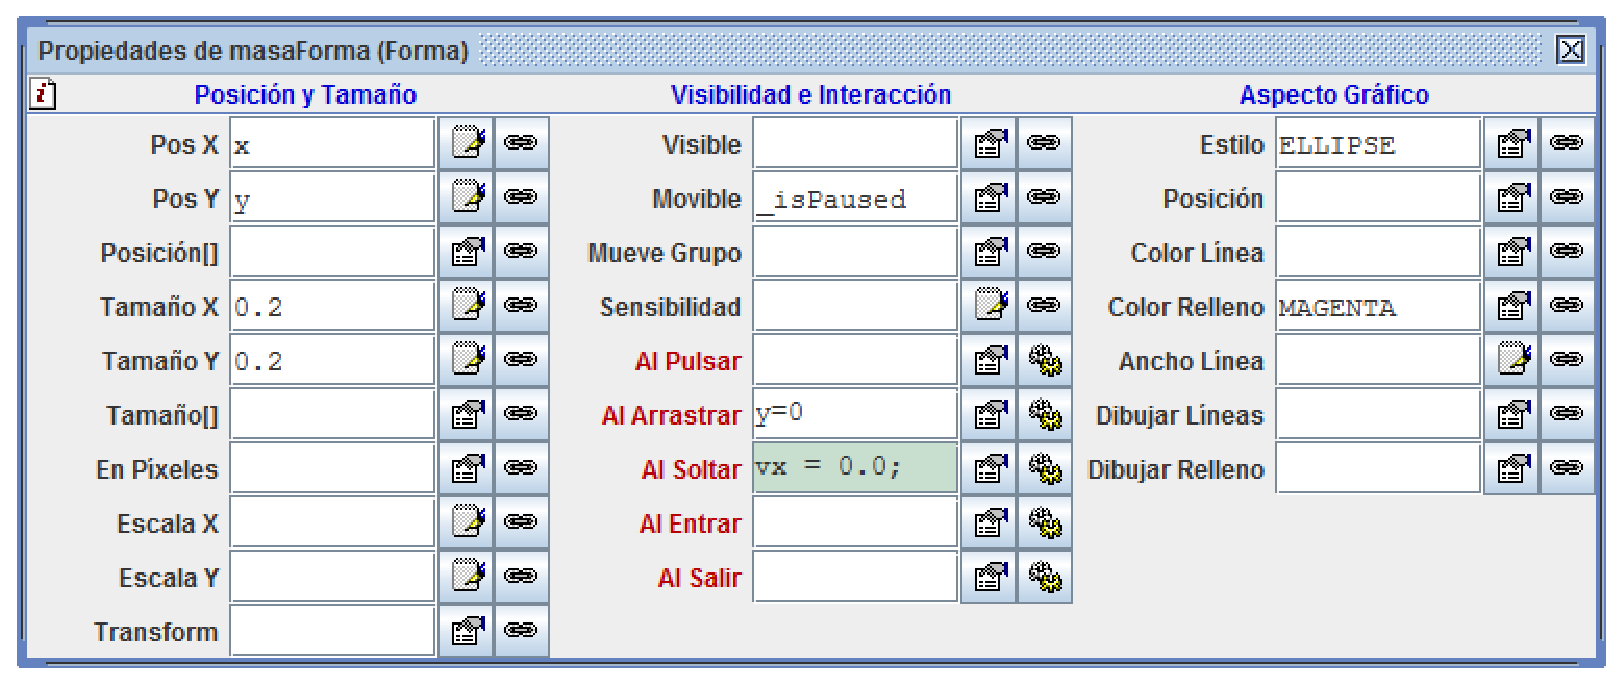
\includegraphics[scale=\scale]{02EjsIntro/images/SpringBallProperties.eps}
    \caption{Tabla de propiedades del elemento \code{masaForma}.}
    \label{fig:02EjsIntro/SpringBallProperties}
\end{figure}

Observe las propiedades que tienen valores constantes. El \code{Estilo}, \code{Tama�o X}, \code{Tama�o Y} y el \code{Color (de) Relleno} producen una elipse de tama�o \code{(0.2,0.2)} unidades (es decir, un c�rculo) relleno de color magenta. Mayor relevancia tiene el hecho de que las propiedades \code{Pos X} y \code{Pos Y} de la forma est�n ligadas a las variables \code{x} e \code{y} del modelo. Esta simple asignaci�n establece una conexi�n bidireccional entre el modelo y la vista. Estas variables cambian conforme el modelo se desarrolla y la forma sigue los valores de \code{x} y de \code{y}. Si el usuario arrastra la forma a una nueva posici�n, las variables \code{x} e \code{y} del modelo tambi�n cambian. N�tese que la propiedad \code{Movible} est� s�lo permitida cuando la animaci�n est� en pausa.

Los elementos pueden tener tambi�n \emph{propiedades de acci�n}\index{Ejs!action properties}, que pueden estar asociadas a c�digo Java. (Las propiedades de acci�n aparecen en letras rojas.) Las acciones del usuario, como arrastrar o hacer clic, llaman a sus correspondientes propiedades de acci�n, de modo que permiten una forma sencilla de controlar la simulaci�n. Si el usuario arrastra la masa, el c�digo que aparece en la propiedad \code{Al Arrastrar} restringe el movimiento de la forma en la direcci�n horizontal obligando a que la variable \code{y} valga \code{0}. Finalmente, cuando se suelta el bot�n del rat�n se ejecuta el siguiente c�digo:

\begin{listing}
\begin{verbatim}
vx = 0.0;            // pone la velocidad a cero
_view.resetTraces(); // limpia todas las gr�ficas
\end{verbatim}
\end{listing}

\noindent Haciendo clic en el icono junto al campo de texto aparece un peque�o editor que muestra este c�digo.

\note{Como el c�digo para la acci�n de \code{Al Soltar} supera el espacio para una l�nea, el fondo del campo aparece m�s oscuro (en verde). Otros tipos de datos como las propiedades booleanas, tienen editores diferentes. Haciendo clic en el segundo icono aparece una ventana de di�logo con una lista de variables y m�todos a elegir para esta propiedad.}

\begin{exercise}[Inspectores de elementos]\label{ex:02EjsIntro/properties}
El inspector de propiedades para la masa muestra distintos tipos de propiedades con sus posibles valores. Explore las propiedades de la vista. Por ejemplo, los elementos \code{desplazamientoRastro} y \code{velocidadRastro} correspondientes a las gr�ficas del desplazamiento y de la velocidad frente al tiempo que puede encontrar en la segunda ventana de la vista. �Cu�l es el m�ximo n�mero de puntos que se pueden a�adir a cada gr�fica?
\end{exercise}

\subsection{La simulaci�n completa}

Hemos visto que \Ejs\ es una poderosa herramienta que nos permite expresar nuestro conocimiento de un modelo con un alto nivel de abstracci�n. Cuando hicimos el modelo de masa y muelle primero creamos una tabla de variables que describiesen el modelo e inicializamos dichas variables utilizando una columna de la tabla. Entonces usamos un panel de evoluci�n con un editor de alto nivel para sistemas de ecuaciones diferenciales ordinarias de primer orden con el fin de especificar c�mo cambiaba su estado respecto al tiempo. Despu�s escribimos relaciones para calcular las variables auxiliares y las de salida que pod�an expresarse utilizando variables de estado. Finalmente, creamos la interfaz gr�fica para el usuario y visualizaciones de alto nivel tan s�lo arrastrando objetos desde la \lit{Paleta} hasta el \lit{�rbol de elementos}. Configuramos las propiedades de los elementos mediante un editor de propiedades y algunas propiedades fueron asociadas con variables del modelo.

Es importante hacer ver que las tres l�neas de c�digo en el panel de relaciones fijas (Figura~\ref{fig:02EjsIntro/ModelRelations}) y las dos l�neas de c�digo del m�todo de acci�n de la forma son el �nico c�digo expl�cito en Java necesario para implementar el modelo. \Ejs\ crea un programa en Java completo, procesando la informaci�n de los paneles de trabajo cuando presionamos el bot�n de ejecuci�n, como se describe en la Secci�n~\ref{section:02Running}.


% -----------------------------------------------------
\section{Ejecutando la simulaci�n}\label{section:02Running}\index{Simulation!running}
% -----------------------------------------------------

Es el momento de ejecutar la simulaci�n haciendo clic en el bot�n de \lit{Ejecuci�n}, 
\includegraphics[scale=\linescale]{images/launch.eps}. \ejs\ genera el c�digo Java y lo compila, recoge archivos auxiliares y de librer�a y ejecuta el programa compilado. Todo con un �nico clic de rat�n.

Al ejecutar la simulaci�n se inicializan sus variables y se eval�an las relaciones fijas para asegurar que el modelo est� en un estado consistente. La evoluci�n respecto del tiempo del modelo empieza cuando el bot�n de marcha/paro de la interfaz del usuario se presiona. (El bot�n marcha/paro muestra el icono 
\includegraphics[scale=\linescale]{images/OSPicons/play.eps} cuando la simulaci�n est� parada y el icono 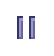
\includegraphics[scale=\linescale]{images/OSPicons/pause.eps} cuando est� en marcha.) En nuestro ejemplo, el programa ejecuta un m�todo num�rico para avanzar la ecuaci�n diferencial del oscilador arm�nico cada $0.05$ unidades de tiempo y ejecuta entonces el c�digo de relaciones. Los datos se pasan entonces al gr�fico y el gr�fico se redibuja. Este proceso se repite $20$ veces por segundo.

Cuando ejecutamos una simulaci�n, \ejs\ cambia el icono de ejecuci�n a color rojo y muestra mensajes de informaci�n diciendo que la simulaci�n se ha generado correctamente y que est� funcionando. Advierta que las dos ventanas de \ejs\ desaparecen y son reemplazadas por unas ventanas nuevas, aunque similares, sin el sufijo en sus t�tulos. Estas vistas s� que responden a las acciones del usuario. Haga clic y arrastre la part�cula hasta la posici�n inicial deseada y entonces pulse en el bot�n de marcha/paro. La masa oscila alrededor de su posici�n de equilibrio y la gr�fica muestra los datos de velocidad y desplazamiento como se muestra en la Figura~\ref{fig:02EjsIntro/SpringRunning}.

Detenga la simulaci�n y haga clic con el bot�n derecho sobre cualquiera de las �reas de dibujo de la simulaci�n. En el men� emergente que aparece seleccione \code{Opciones de los elementos->panelConEjes->Herramientas de Datos} y pulse para mostrar y analizar los datos generados por el modelo. Este mismo men� ofrece otras opciones sobre la ejecuci�n, como la captura de pantalla. Para salir del programa, cierre la ventana principal de la simulaci�n.

\begin{figure}[htb]
  \centering
  \subfigure{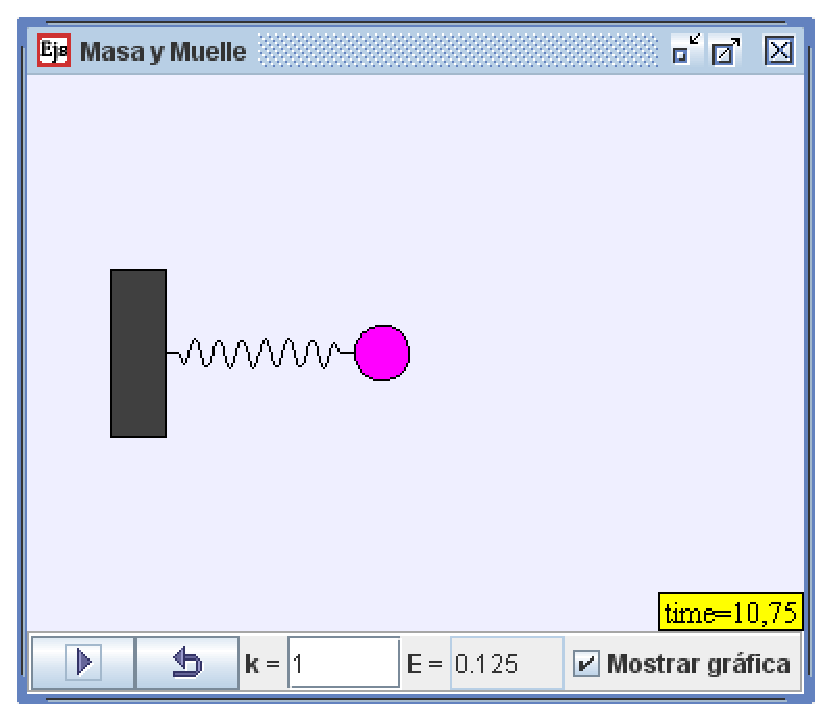
\includegraphics[scale=\scale]{02EjsIntro/images/SpringRunning1.eps}}
  \subfigure{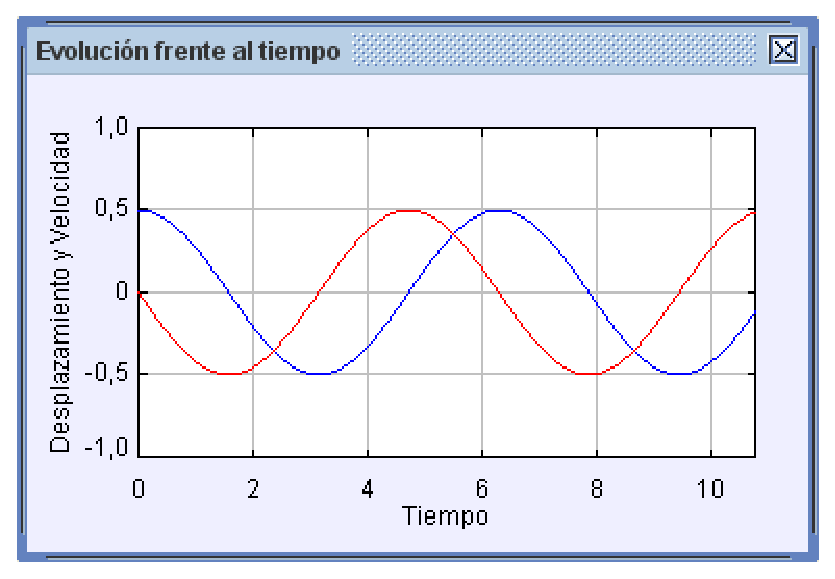
\includegraphics[scale=\scale]{02EjsIntro/images/SpringRunning2.eps}}
  \caption{ La simulaci�n de masa y muelle muestra un dibujo interactivo del modelo y una gr�fica con los datos de desplazamiento y velocidad.}
  \label{fig:02EjsIntro/SpringRunning}
\end{figure}


% -----------------------------------------------------
\section{Distribuci�n de la simulaci�n}\label{section:02Distributing}\index{Simulation!distribution}
%

Las simulaciones creadas con \ejs\ son por s� mismas programas Java independientes que pueden distribuirse sin necesidad de que los destinatarios utilicen \ejs. La forma m�s sencilla para hacer esto es empaquetar la simulaci�n en un �nico archivo ejecutable de tipo jar haciendo clic en el icono \lit{Empaquetar}, 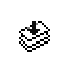
\includegraphics[scale=\linescale]{images/package.eps}. Aparece una explorador de archivos que le permitir� elegir un nombre para el paquete jar. La direcci�n por defecto donde se situar� este archivo es el directorio \file{export} de su espacio de trabajo, pero puede elegir tanto el directorio como el nombre del paquete. Este archivo independiente est� preparado para ser distribuido en un CD o via Internet. Otros mecanismos de distribuci�n est�n disponibles  haciendo clic con el bot�n derecho en el icono como se describe en el Ap�ndice~\ref{appendix:Distribution}.

\begin{exercise}[Distribuci�n del modelo]\label{ex:02EjsIntro/distribution}
Haga clic en el icono \lit{Empaquetar} de la barra de tareas para crear un archivo jar independiente con la simulaci�n de masa y muelle. Copie este archivo jar en un directorio de trabajo diferente del de su instalaci�n de \ejs. Cierre \ejs\ y verifique que la simulaci�n funciona como una aplicaci�n independiente.\end{exercise}

Aunque el archivo jar de nuestra simulaci�n est� listo para ser usado y distribuido, un importante hecho pedag�gico es que este archivo jar se ha creado de tal manera que los usuarios puedan volver a \ejs\ en cualquier momento para examinar, modificar y adaptar el modelo. (Siempre y cuando se tenga \ejs\ instalado, por supuesto.) El archivo jar contiene un peque�a descripci�n en \emph{Lenguaje de Marcas Ampliable} (XML) de cada modelo y haciendo clic con el bot�n derecho en un panel de dibujo del modelo se obtiene un men� desplegable con una opci�n para copiar el archivo en \ejs. Esta acci�n extraer� los archivos necesarios del archivo jar, buscar� \ejs\ en el disco duro del usuario, copiar� los archivos en la localizaci�n correcta y ejecutar� \ejs\ con la simulaci�n cargada. Si ya existiera un modelo con el mismo nombre, este puede ser reemplazado. El usuario puede inspeccionar, ejecutar y modificar el modelo tal y como hemos hecho en este cap�tulo. Un estudiante puede, por ejemplo, conseguir un modelo o una plantilla por parte del profesor y m�s tarde reempaquetar el modelo una vez modificado en un nuevo archivo jar como propuesta de un ejercicio completo.

\begin{exercise}[Extraer un modelo]\label{ex:02EjsIntro/redistribution}
Ejecute el archivo jar independiente que contiene el modelo de masa y muelle creado en el Ejercicio~\ref{ex:02EjsIntro/distribution}. Haga clic con el bot�n derecho sobre la gr�fica o el dibujo del modelo y seleccione el item \lit{Abrir Modelo \ejs} del men� desplegable para copiar el modelo empaquetado de vuelta a \ejs.
\end{exercise}

\ejs\ ha sido dise�ado para ser al mismo tiempo una herramienta de modelado y de autor, y proponemos ahora que experimente con ella para aprender c�mo puede usted crear y distribuir sus propios modelos. Para empezar, recomendamos que ejecute la simulaci�n de masa y muelle y realice las actividades de la segunda p�gina del panel de \lit{Descripci�n}. En la siguiente secci�n modificaremos la simulaci�n.


% -----------------------------------------------------
\section{Modificando la simulaci�n}\label{section:02Modifying}
% -----------------------------------------------------

Como hemos visto, una caracter�stica importante y distintiva de \Ejs\ es que nos permite crear y estudiar una simulaci�n con un alto nivel de abstracci�n. En la secci�n anterior, hemos inspeccionado un modelo existente de una masa y un muelle, as� como su interfaz de usuario. Ahora vamos a mostrar otras capacidades adicionales de \Ejs\ a�adiendo fricci�n y una fuerza externa al modelo, as� como la visualizaci�n del espacio de fases del sistema.

\subsection{Extendiendo el modelo}\label{section:02ModifyingModel}

Podemos a�adir rozamiento en nuestro modelo introduciendo una fuerza viscosa (ley de Stoke) que es proporcional al opuesto de la velocidad $F_f = - b\,v_x$, donde $b$ es el coeficiente de rozamiento. Tambien a�adimos una fuerza externa, dependiente del tiempo, que toma la forma de una funci�n sinusoidal $F_e(t)=A\,\sin(\omega\, t)$. La inclusi�n de estas fuerzas cambia la ecuaci�n diferencial de segundo orden \eqref{eq:02EjsIntro/SpringBasic} a:
\begin{equation}
  \frac{d^2\ x}{dt^2} = -\frac{k}{m}\,(x-L) - \frac{b}{m}\,\frac{d\ x}{dt} + \frac{1}{m}\,F_e(t), \label{eq:02EjsIntro/SpringComplete}
\end{equation}
o, como en las ecuaciones \eqref{eq:02EjsIntro/SpringBasicODE1} y \eqref{eq:02EjsIntro/SpringBasicODE2},
\begin{eqnarray}
  \frac{d\ x} {dt} &=& v_x,                  \label{eq:02EjsIntro/SpringCompleteODE1} \\
  \frac{d\ v_x}{dt} &=& -\frac{k}{m}\,(x-L) - \frac{b}{m}\,v_x + \frac{1}{m}\,F_e(t). \label{eq:02EjsIntro/SpringCompleteODE2}
\end{eqnarray}

\subsubsection{A�adiendo variables}

Introducir nuevas fuerzas requiere que a�adamos variables para el coeficiente de fricci�n din�mica y para la amplitud y frecuencia de la fuerza externa sinusoidal. Vuelva al panel del \lit{Modelo} de \ejs\ y seleccione su panel de \lit{Variables}. Haga clic con el bot�n derecho en la pesta�a de la p�gina de variables existente para ver su men� desplegable, como en la Figura~\ref{fig:02EjsIntro/ModifyVariables1}. Seleccione \lit{A�adir una p�gina}. Introduzca como nombre de la nueva tabla \code{Fricci�n y fuerza} y aparecer� una tabla vac�a.

\begin{figure}[htb]
    \centering
  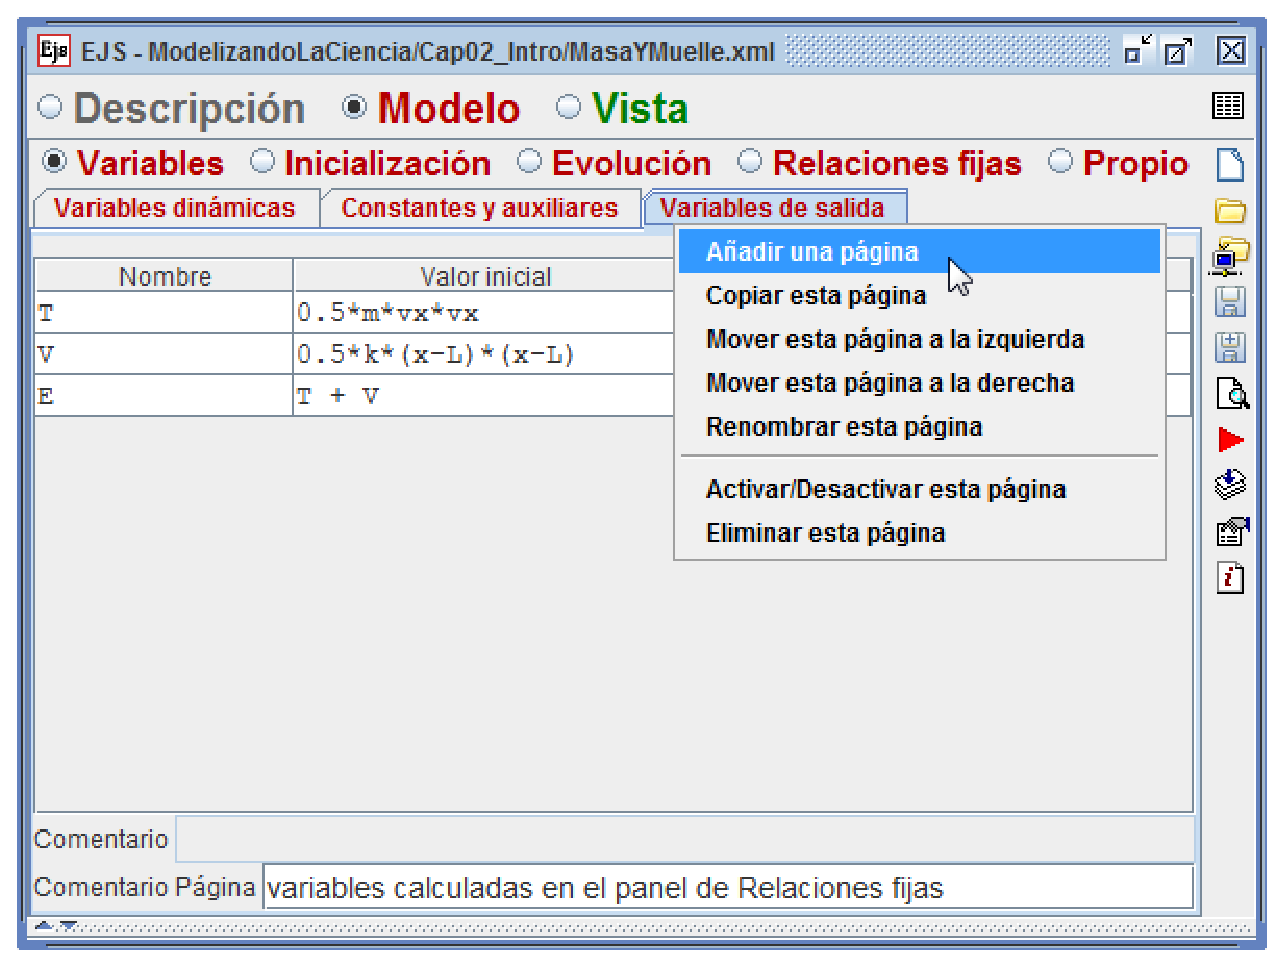
\includegraphics[scale=\scale]{02EjsIntro/images/ModifyVariables1.eps}
    \caption{El men� desplegable de una p�gina de variables.}
    \label{fig:02EjsIntro/ModifyVariables1}
\end{figure}

Ahora usamos la nueva tabla para declarar las variables que necesitamos. Podr�amos haber usado una de las tablas ya existentes, pero declararlas en varias p�ginas nos ayuda a organizar mejor las variables por categor�as. Haga doble clic en una de las celdas de la tabla para hacerla editable y mu�vase a trav�s de la tabla utilizando las flechas o el tabulador. Escriba \code{b} en la celda destinada al \lit{Nombre} de la primera fila, e introduzca el valor \code{0.1} en la celda \lit{Valor inicial} justo a su derecha. No necesitamos hacer nada m�s, ya que el \lit{Tipo} elegido ya es correcto. \ejs\ comprueba la sintaxis del valor introducido y lo eval�a. Si introducimos un valor err�neo, el fondo de la celda se mostrar� en color rosa.

N�tese que cuando rellene el nombre de una nueva variable aparece una nueva fila autom�ticamente. Proceda de forma similar para declarar una nueva variable para la amplitud de la fuerza externa (\code{amp}) con valor \code{0.2} y para su frecuencia (\code{frec}) con valor \code{2.0}. Puede dejar una explicaci�n sobre el significado de estas variables escribiendo un peque�o comentario para cada una de ellas en la parte inferior de la tabla. Nuestra nueva tabla de variables se muestra en la Figura~\ref{fig:02EjsIntro/ModifyVariables2}. Puede ignorar la fila vac�a del final de la tabla o eliminarla haciendo clic con el bot�n derecho sobre esta fila y seleccionando \lit{Eliminar} del men� desplegable que aparece.

\begin{figure}[htb]
    \centering
  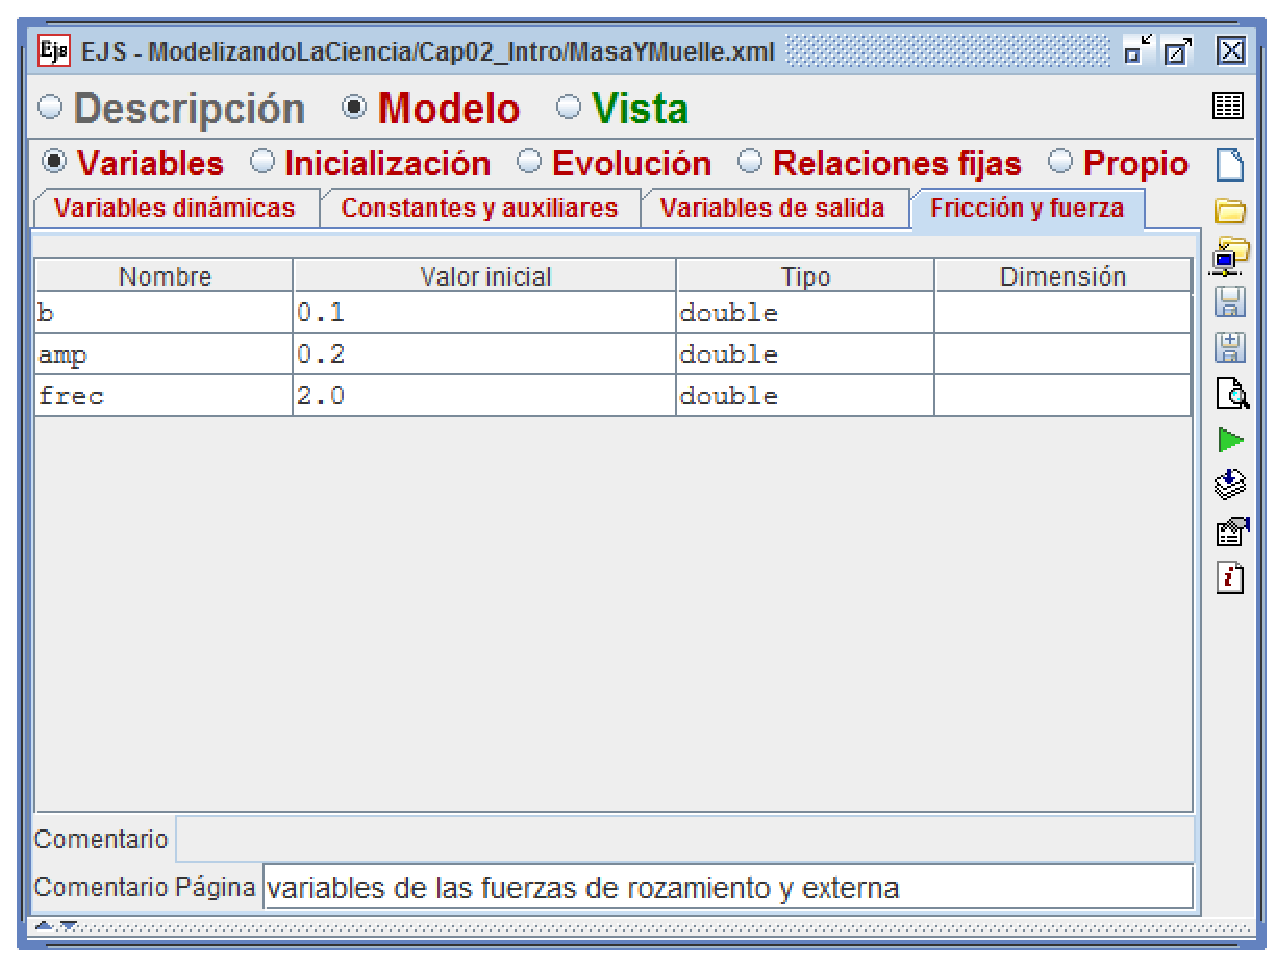
\includegraphics[scale=\scale]{02EjsIntro/images/ModifyVariables2.eps}
    \caption{La nueva tabla de variables para los t�rminos del rozamiento y la fuerza externa.}
    \label{fig:02EjsIntro/ModifyVariables2}
\end{figure}

\subsubsection{Modificando la evoluci�n}

Ahora, vamos a modificar la ecuaci�n diferencial de la p�gina de evoluci�n a�adiendo expresiones para los nuevos t�rminos de la ecuaci�n \eqref{eq:02EjsIntro/SpringCompleteODE2}. Vaya al panel de \lit{Evoluci�n}, haga doble clic en la celda de \lit{Derivada} de la segunda ecuaci�n y escriba:

\begin{listing}
\begin{verbatim}
-k/m * (x-L) - b*vx/m + fuerza(t)/m
\end{verbatim}
\end{listing}
D�se cuenta de que utilizamos un m�todo (funci�n) llamado \code{fuerza} que no ha sido definido todav�a. Podr�amos haber escrito directamente una expresi�n expl�cita para la funci�n sinusoidal. Sin embargo, definimos un m�todo fuerza para que quede un c�digo m�s limpio y f�cil de leer y que adem�s nos permita discutir ahora los m�todos propios.

\subsubsection{A�adiendo m�todos propios}

El m�todo \code{fuerza} se define usando el panel \lit{Propio} del modelo. Vaya a este panel y haga clic en el �rea central que estar� vac�a para crear una nueva p�gina de c�digo propio. Llame a la p�gina \lit{fuerza}. Notar� que la p�gina se crea con un c�digo plantilla que define el m�todo. Edite el c�digo para que se lea:

\begin{listing}
\begin{verbatim}
public double fuerza (double tiempo) {
  return amp*Math.sin(frec*tiempo); // fuerza externa sinusoidal
}
\end{verbatim}
\end{listing}
Teclee este c�digo exactamente como se muestra aqu�, incluyendo las may�sculas. El compilador producir� errores al generar la simulaci�n si hay cualquier error de sintaxis.

Observe que estamos pasamos al m�todo \code{fuerza}, como par�metro de entrada, el valor del tiempo que queremos utilizar para calcular la fuerza externa. Pasarle el valor del tiempo es importante. Ser�a incorrecto pedirle al m�todo que usase el valor de la variable t como sigue:

\begin{listing}
\begin{verbatim}
public double fuerza () {
  return amp*Math.sin(frec*t);// implementaci�n incorrecta del m�todo
}
\end{verbatim}
\end{listing}

\noindent La raz�n de que debamos pasar el tiempo como par�metro es que el tiempo cambia a lo largo del paso de la evoluci�n. Para que el algoritmo de resoluci�n de la ecuaci�n diferencial calcule correctamente la fuerza dependiente del tiempo en instantes intermedios de un paso de integraci�n num�rica, el tiempo debe pasarse al m�todo que calcula la derivada.

\note{Las variables que cambian (evolucionan) deben pasarse a los m�todos que se usan en el c�lculo de la derivada porque los m�todos num�ricos eval�an la columna \lit{Derivada} en el panel de trabajo de las EDO en valores intermedios entre $t$ y $t+dt$. (v�ase el capitulo~\ref{chapter:ODE}.) En otras palabras, la variable independiente y cualquier otra variable din�mica que aparezca en la columna \lit{Estado} del editor de EDO debe pasarse a cualquier m�todo al que se haga referencia en la columna \lit{Derivada}. Aquellas variables que permanecen constantes  durante el paso de evoluci�n podr�an utilizarse sin ser pasadas por par�metros de entrada ya que se puede utilizar el valor que ten�a la variable al inicio del paso.}

\subsection{Mejorando la Vista}\label{section:02ModifyingView}

Ahora vamos a a�adir a la \lit{Vista} una visualizaci�n del espacio de fases (desplazamiento frente a velocidad) de la evoluci�n del sistema. Tambi�n vamos a a�adir campos de entrada para mostrar y modificar el valor de los par�metros de rozamiento, amplitud y frecuencia.

Vaya al panel de la \lit{Vista} y f�jese que la paleta de \lit{Interfaz} contiene varios subpaneles. Haga clic en la pesta�a con el icono 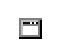
\includegraphics[scale=\linescale]{images/Groups/Containers.eps} para mostrar la paleta \lit{Ventanas, contenedores y paneles de dibujo}. Haga clic en el icono de Panel con ejes, 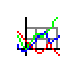
\includegraphics[scale=\linescale]{images/Elements/PlottingPanel.eps}, en esta misma paleta. Puede mantener el cursor sobre cualquiera de los iconos para que se muestre una nota que describe el elemento brevemente en caso de que tenga dificultades para reconocer el icono. Al seleccionar un elemento, �ste muestra un marco de color alrededor del icono en la paleta y el cursor se convierte en una varita m�gica, 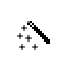
\includegraphics[scale=\linescale]{images/create.eps}. Estos cambios indican que \ejs\ est� listo para crear un elemento del tipo seleccionado.

Haga clic en el elemento \code{ventanaDialogo} en el \lit{�rbol de elementos} como muestra la Figura~\ref{fig:02EjsIntro/ModifyViewAddPlottingPanel} para a�adir un panel con ejes a la vista.

\begin{figure}[htb]
    \centering
  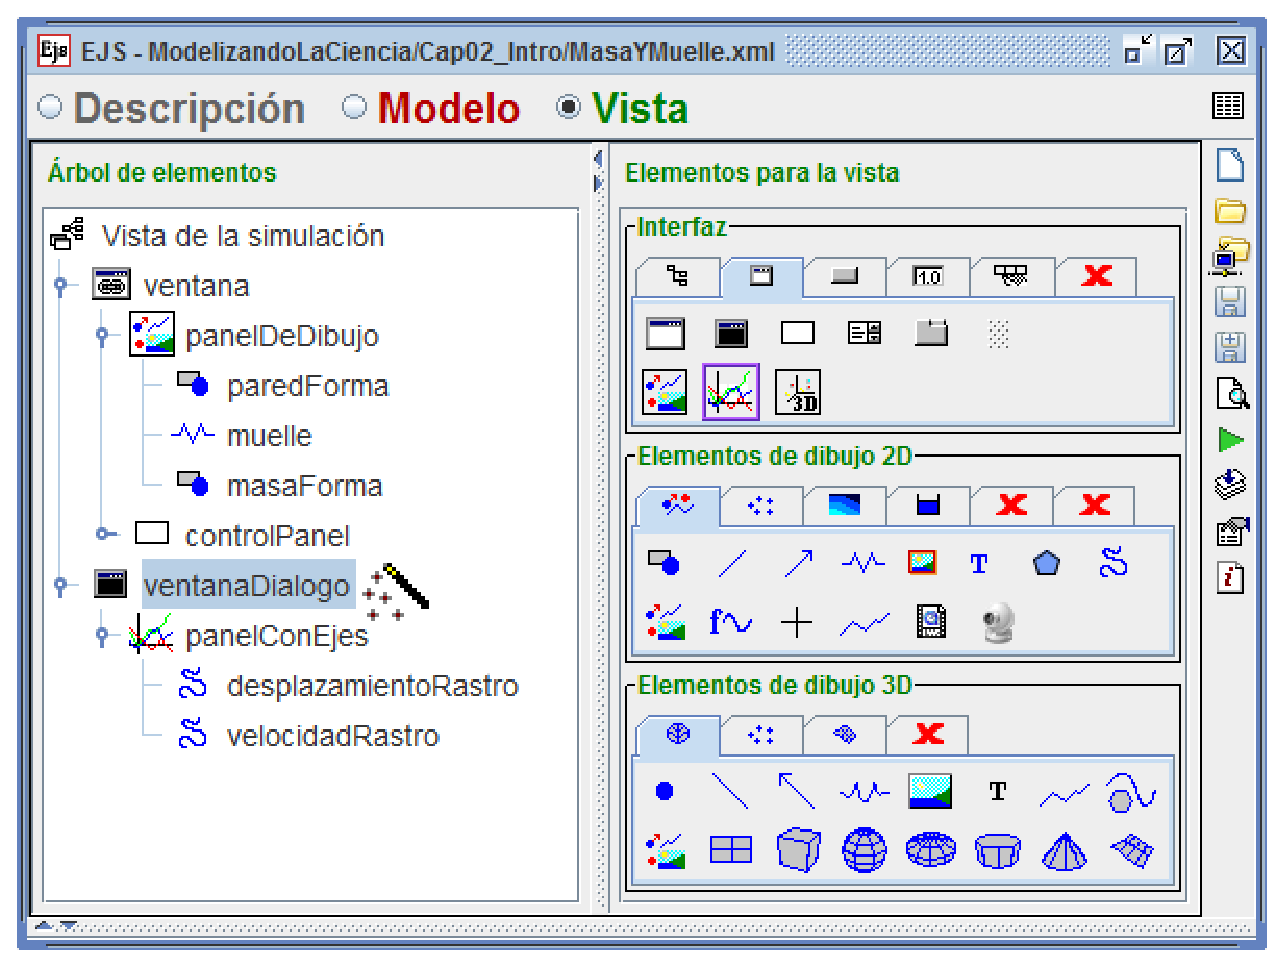
\includegraphics[scale=\scale]{02EjsIntro/images/ModifyViewAddPlottingPanel.eps}
    \caption{Creaci�n de un panel con ejes como hijo del elemento \code{di�logo} de la vista.}
    \label{fig:02EjsIntro/ModifyViewAddPlottingPanel}
\end{figure}

\ejs\ nos pide un nombre para el nuevo elemento y entonces lo crea como hijo del ya existente, \code{ventanaDialogo}. Aparece una nueva gr�fica, pero la ventana de di�logo es demasiado peque�a. Vuelva al modo de dise�o (l�brese de la varita m�gica) haciendo clic en cualquier �rea en blanco del \lit{�rbol de elementos} o presionando la tecla \lit{Esc}. Puede reescalar la ventana arrastrando su esquina o haciendo doble clic en el elemento \code{ventanaDialogo} en el �rbol para mostrar su tabla de propiedades y cambiar alli su \code{Tama�o} a \texttt{"385,530"} de forma que doblar� su altura. Finalmente, edite la tabla de propiedades  del panel con ejes reci�n creado para cambiar el \code{T�tulo} a \code{Espacio de fases}, el \code{T�tulo X} a \code{Desplazamiento} y el \code{T�tulo Y} a \code{Velocidad}. (\ejs\ a�adir� comillas a estas cadenas de texto para adecuarse a la sintaxis de Java.) Seleccione el m�nimo y m�ximo para las escalas X e Y en \code{-1} y \code{1}, respectivamente, y deje las otras propiedades tal y como est�n.

El panel con ejes es un contenedor para la gr�fica del espacio de fases. Los datos del espacio de fases se dibujan en este panel utilizando un elemento del tipo \code{Rastro}, 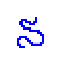
\includegraphics[scale=\linescale]{images/Elements/Trail.eps}. Encuentre el elemento \code{Traza} en la \code{Paleta de Elementos de Dibujo 2D} y cree un elemento de este tipo haciendo clic con la varita m�gica sobre el panel de espacio de fases. Finalmente, edite las propiedades del nuevo elemento para establecer su \code{Entrada X} a \code{x - L} y su \code{Entrada Y} a \code{vx}. Estas asignaciones hacen que la simulaci�n  a�ada un nuevo punto \code{(x - L,vx)} a la traza despu�s de cada paso de evoluci�n, de forma que se dibuje la gr�fica de espacio de fases que se muestra en la Figura~\ref{fig:02EjsIntro/ModifyRunning}.

\begin{figure}[htb]
  \centering
  \subfigure{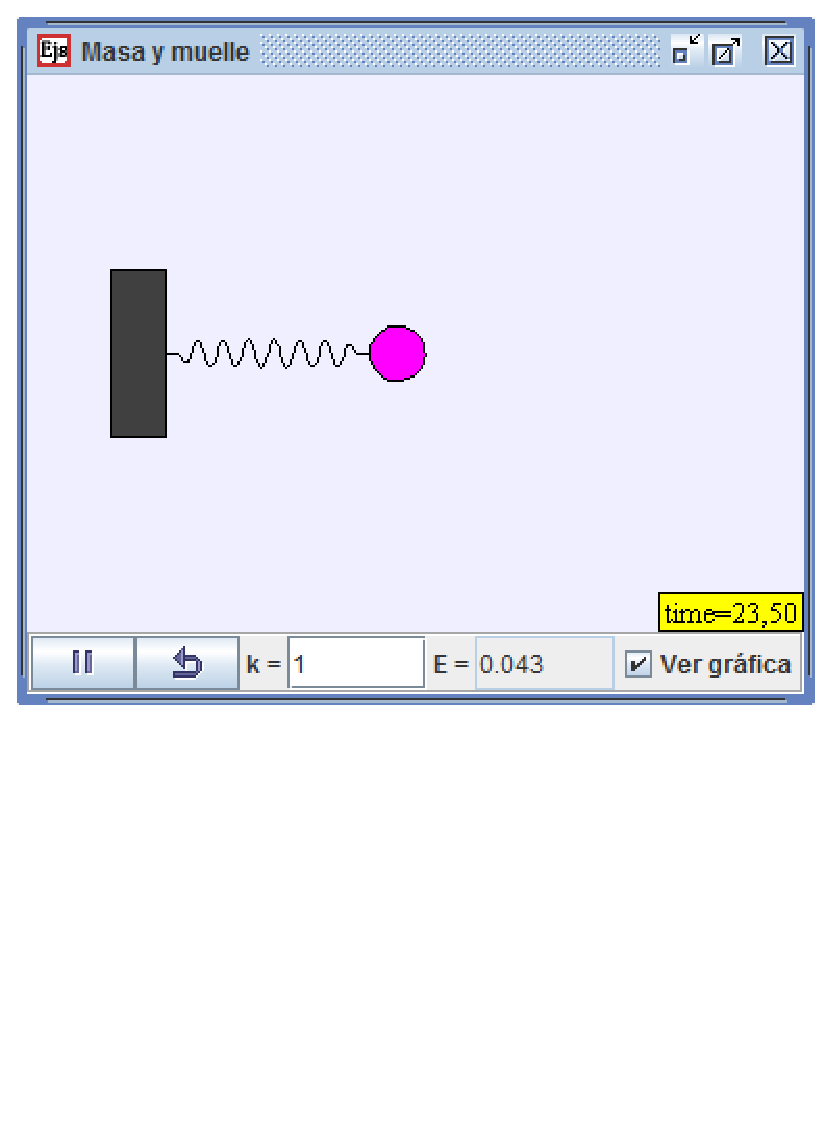
\includegraphics[scale=\scale]{02EjsIntro/images/ModifyRunning1.eps}}
  \subfigure{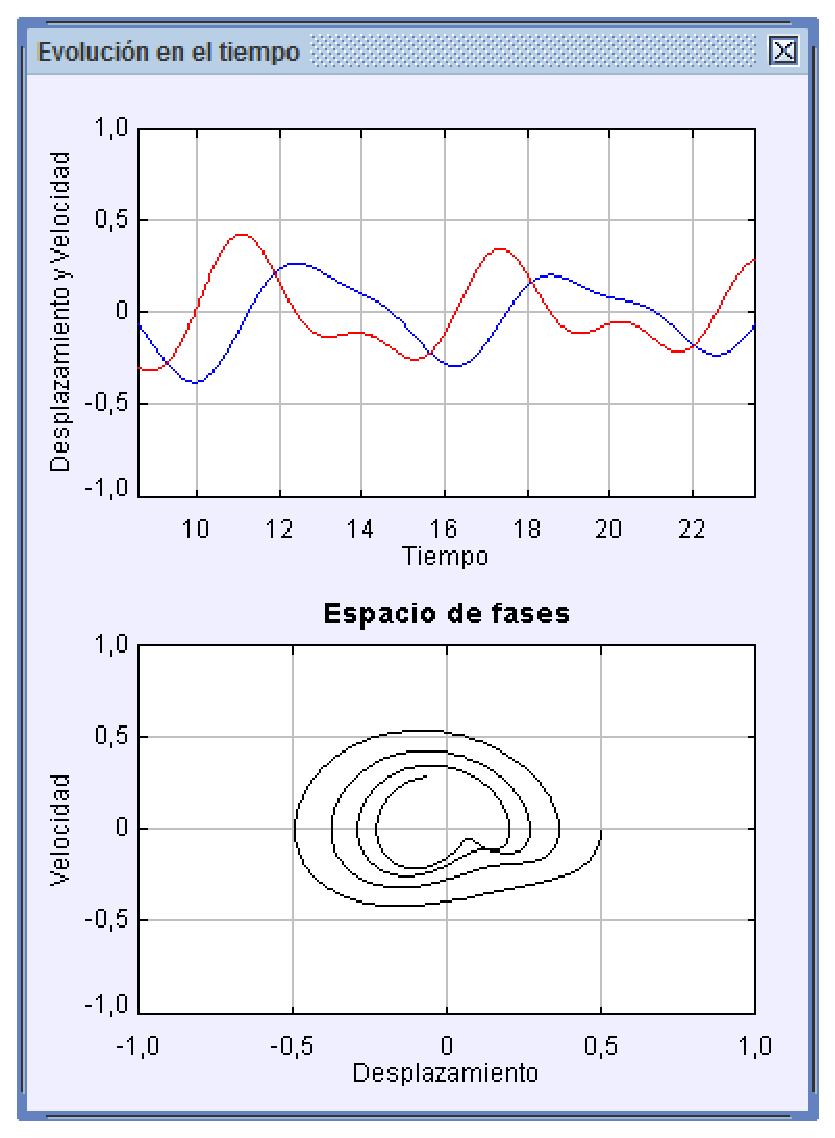
\includegraphics[scale=\scale]{02EjsIntro/images/ModifyRunning2.eps}}
  \caption{La simulaci�n modificada. La ventana de di�logo incluye ahora una gr�fica frente al tiempo y una gr�fica del espacio de fases.}
  \label{fig:02EjsIntro/ModifyRunning}
\end{figure}

Para terminar con las modificaciones, vamos a a�adir un nuevo panel en la parte superior de la imagen que muestre los par�metros de la fuerza externa sinusoidal.

\begin{bulletlist}

\item Seleccione el icono de \code{Panel}, 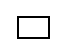
\includegraphics[scale=\linescale]{images/Elements/Panel.eps}, en el grupo de \lit{Ventanas, contenedores y paneles de dibujo} dentro de la paleta \lit{Interfaz}. Haga clic con la varita m�gica en el elemento llamado \code{ventana} en el \lit{�rbol de elementos} para crear un nuevo panel llamado \code{paramFuerzaPanel} en la parte superior de la ventana. Utilice el inspector de propiedades para elegir el dise�o del panel como \lit{FLOW:center,0,0} y su tipo de borde como \texttt{LOWERED\_ETCHED}.
\item Seleccione el icono del elemento \code{Etiqueta}, 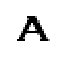
\includegraphics[scale=\linescale]{images/Elements/Label.eps}, en el subgrupo \lit{Botones y decoraci�n} de la paleta de \lit{Interfaz} y cree un nuevo elemento de este tipo en el panel de par�metros de la fuerza. Cambie el texto de la etiqueta a \texttt{"frecuencia="}.
\item Seleccione el elemento de \code{Campo Num�rico}, 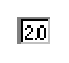
\includegraphics[scale=\linescale]{images/Elements/ParsedField.eps}, y cree un nuevo elemento llamado \code{frecCampo} en el panel de par�metros de la fuerza. Edite su tabla de propiedades como muestra la Figura~\ref{fig:02EjsIntro/ModifyField}. La conexi�n con la variable \code{frec} se establece usando la propiedad \code{Variable}. Haga clic en el segundo icono de la derecha del campo de texto de la propiedad, 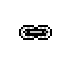
\includegraphics[scale=\linescale]{images/link.eps}, y elija la variable apropiada. La lista de variables muestra todas las variables del modelo que pueden ser utilizadas en este campo. La propiedad \code{Formato} indica el n�mero de cifras decimales que desea que muestre el valor de la variable.
\item Repita todo el proceso para a�adir la variable \code{amp} a la interfaz de usuario.
\end{bulletlist}

\begin{figure}[htb]
    \centering
  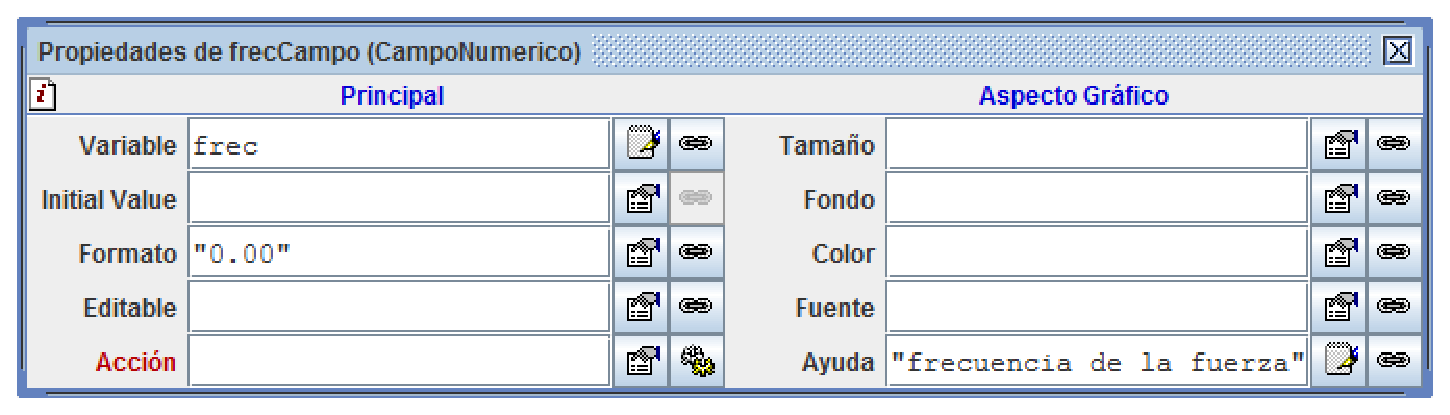
\includegraphics[scale=\scale]{02EjsIntro/images/ModifyField.eps}
    \caption{Tabla de propiedades del elemento \code{freqCampo}.}
    \label{fig:02EjsIntro/ModifyField}
\end{figure}

\subsection{Cambiando la descripci�n}\label{section:02ModifyingDescription}

Ahora que hemos cambiado el modelo y su vista deber�amos modificar tambi�n las p�ginas de descripci�n de nuestra simulaci�n. Vaya al panel de trabajo \lit{Descripci�n} y haga clic con el bot�n derecho sobre la pesta�a de la primera p�gina, con el nombre \code{Introducci�n}, para mostrar el men� desplegable para esa p�gina. Seleccione la opci�n \lit{Editar/Ver} esta p�gina. La p�gina de descripci�n cambiar� al modo de edici�n, tal y como muestra la Figura~\ref{fig:02EjsIntro/ModifyHTML}, y aparecer� un sencillo editor que proporciona acceso directo a las funciones m�s comunes de HTML.

Si prefiere usted usar su propio editor, puede copiar y pegar fragmentos de HTML desde su editor al editor de \ejs. Si conoce la sintaxis HTML puede adem�s editar el c�digo fuente directamente haciendo clic sobre el icono 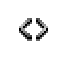
\includegraphics[scale=\linescale]{02EjsIntro/images/SourceHK.eps} en la barra de utilidades. Puede adem�s importar p�ginas HTML completas a \ejs\ haciendo clic con el bot�n derecho sobre una de las pesta�as del panel.

\begin{figure}[htb]
    \centering
  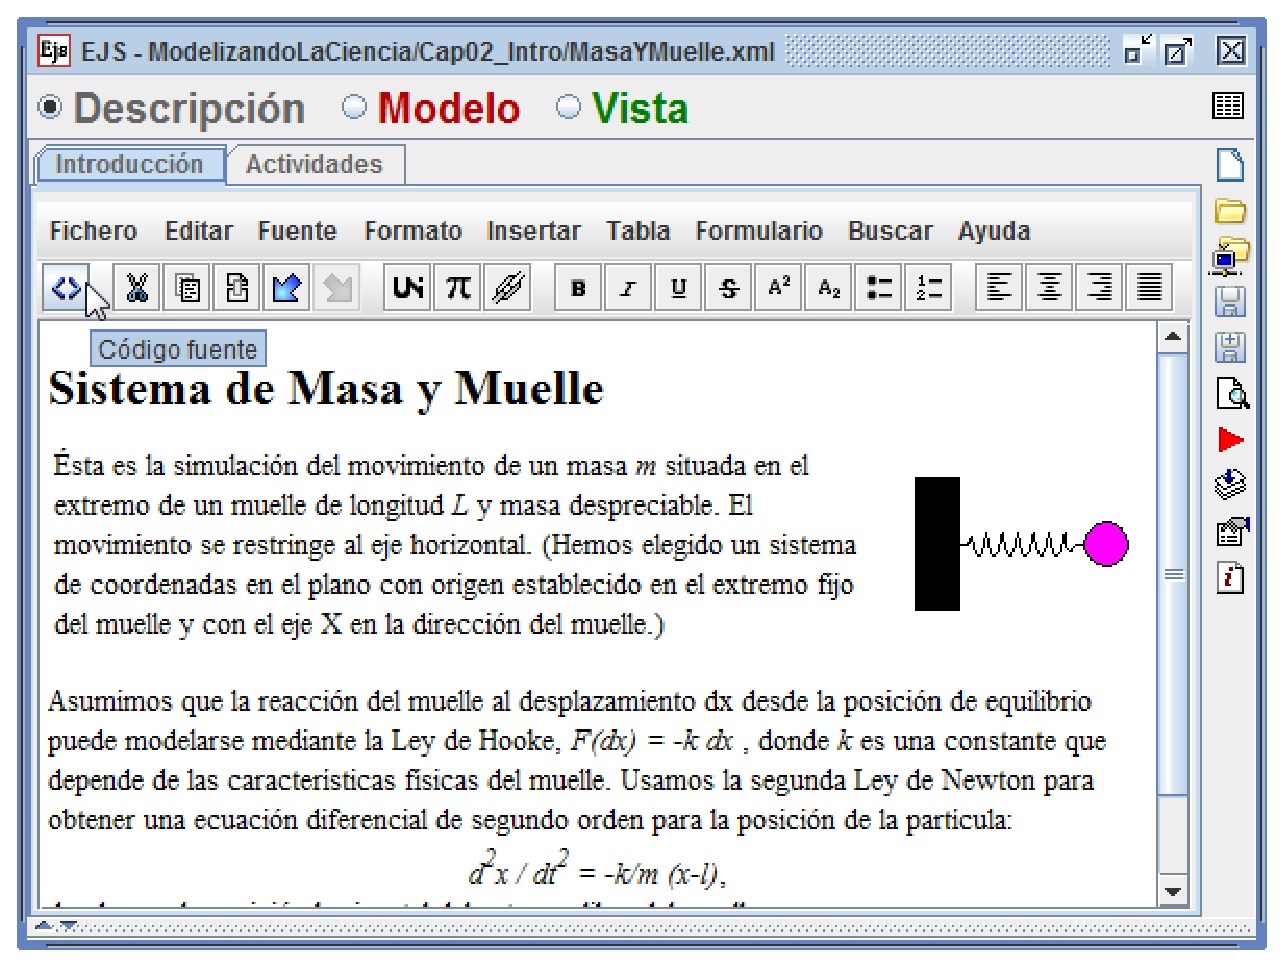
\includegraphics[scale=\scale]{02EjsIntro/images/ModifyHTML.eps}
    \caption{El editor de HTML de \ejs. El cursor se�ala el icono para cambiar al modo de edici�n de c�digo fuente.}
    \label{fig:02EjsIntro/ModifyHTML}
\end{figure}

Edite las p�ginas de descripci�n como crea conveniente. Al menos cambie la discusi�n del modelo para incluir el rozamiento y la fuerza externa. Cuando haya terminado, guarde la nueva simulaci�n con un nombre diferente haciendo clic sobre el icono \lit{Guardar Como} de la barra de tareas de \ejs, 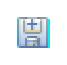
\includegraphics[scale=\linescale]{images/saveAsSmall.eps}. Cuando se le pida, introduzca un nuevo nombre para el archivo XML de su simulaci�n. Nosotros guardamos la simulaci�n modificada en el archivo \file{MasaYMuelleCompleto.xml} en el directorio de este cap�tulo.


% -----------------------------------------------------
\section{Buscando modelos}\label{section:02FindingModels}
% -----------------------------------------------------

Ahora que hemos cubierto los aspectos b�sicos de \ejs\ y ya sabe c�mo cargar, inspeccionar, ejecutar y hasta modificar un ejemplo, puede que est� interesado en encontrar m�s ejemplos para ver qu� han hecho otros usuarios con \ejs. Es posible que pueda encontrar un modelo existente que se ajuste a sus necesidades o que pueda usted modificar f�cilmente para usarlo en sus clases.

Hay dos sitios donde puede usted mirar en busca de m�s modelos.
El primer sitio a mirar es el directorio \file{source} de muestra que viene con su distribuci�n de \ejs. En el directorio \file{source} del espacio de trabajo de la distribuci�n encontrar� algunos subdirectorios con simulaciones de muestra. Estos directorios de muestra se copiaron tambi�n en su propio espacio de trabajo (salvo que indicara usted lo contrario) cuando ejecut� \ejs\ por primera vez.

El segundo, y quiz� m�s interesante, lugar (de hecho, lugares) para buscar nuevos modelos est� accesible a trav�s de Internet. El icono de la barra de herramientas de \ejs\ de librer�as digitales, 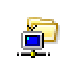
\includegraphics[scale=\linescale]{images/netOpen.eps}, abre una ventana que le permite conectar con repositorios de modelos de \ejs\ accesibles a trav�s de Internet. Esta ventana, que se muestra en la Figura~\ref{fig:02EjsIntro/EJSDigitalLibraries}, contiene un selector en su parte superior con la lista de librer�as digitales disponibles. Seleccione una de estas librer�as o haga clic en el bot�n \lit{Leer el cat�logo} para obtener el listado de modelos de \ejs\ en ella. Todas las librer�as funcionan de manera similar. Nosotros usaremos el repositorio de la librer�a digital \textbf{comPADRE} para ilustrar c�mo se accede a ellas desde \ejs.

\begin{figure}[htb]
    \centering
  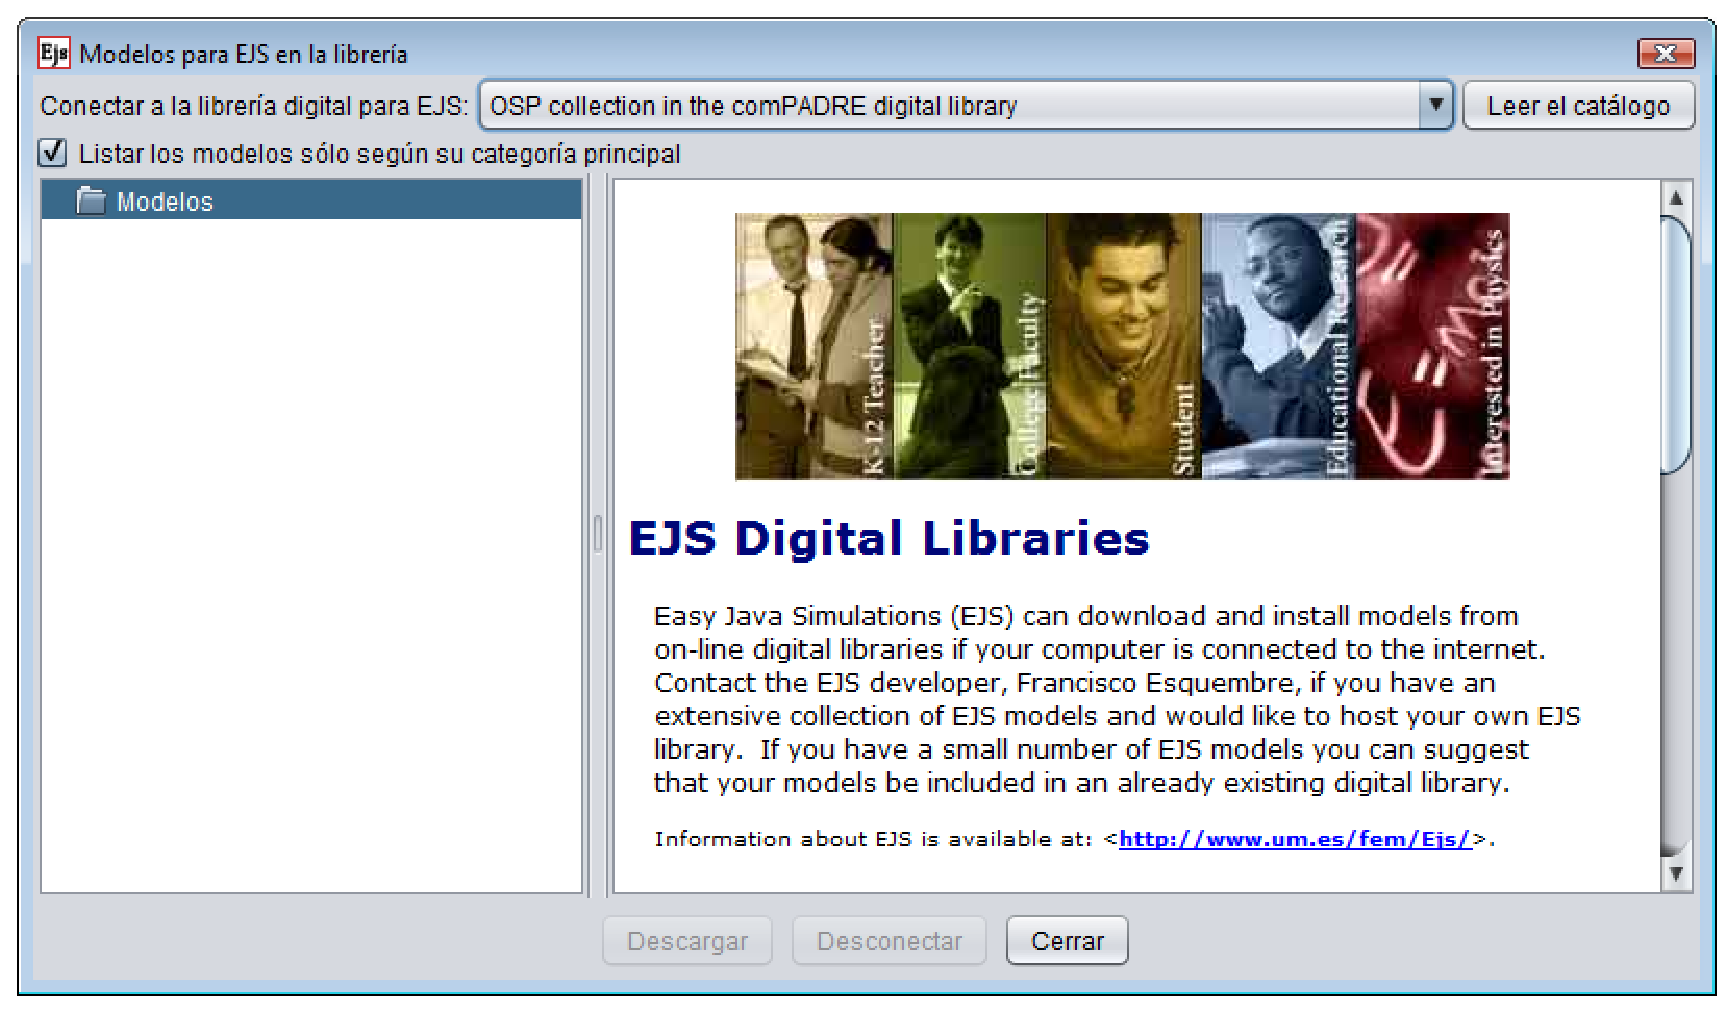
\includegraphics[scale=\scale]{02EjsIntro/images/EJSDigitalLibraries.eps}
    \caption{La ventana de \ejs\ de librer�as digitales. Seleccione uno de los repositorios disponibles usando el selector en la parte superior de la ventana, o haga clic en el bot�n \lit{Leer el cat�logo} para obtener el listado de modelos disponibles.}
    \label{fig:02EjsIntro/EJSDigitalLibraries}
\end{figure}

La librer�a \textbf{comPADRE Pathway}, que es parte de la Librer�a Digital de Ciencia de los Estados Unidos de Am�rica, es una red en expansi�n de colecciones de recursos educativos que sirven de apoyo a profesores y estudiantes de F�sica y Astronom�a. De especial relevancia para nosotros es la colecci�n Open Source Physics en comPADRE, disponible en \link{http://www.compadre.org/OSP}. Esta colecci�n (en ingl�s) contiene recursos computacionales para la ense�anza en forma de simulaciones ejecutables y recursos curriculares que involucran a los estudiantes en actividades de f�sica, computaci�n y modelado por computadora. En particular, contiene modelos de \ejs\ a cuyos archivos de c�digo fuente (XML) puede accederse directamente desde \ejs\ usando el icono de librer�as digitales.

Si est� conectado a Internet, seleccione la entrada \lit{OSP collection on the comPADRE digital library} del selector y \ejs\ se conectar� a la librer�a para obtener el m�s reciente cat�logo de modelos de \ejs\ en esta librer�a. En el momento de escribir estas l�neas, hay cerca de 90 modelos organizados en diferentes categor�as y subcategor�as, y se espera que la colecci�n siga creciendo. Como muestra el marco izquierdo de la Figura~\ref{fig:02EjsIntro/OSPCollection}, la colecci�n est� organizada en categor�as y subcategor�as. Cuando el nombre de una subcategor�a aparezca en rojo, haga doble-clic sobre �l para expandir el nodo con la lista de modelos de la subcategor�a. Como muchos modelos tienen clasificiones principal y secundarias, el bot�n selector en la parte superior, justo debajo del selector de librer�a, le permite decidir si quiere que los modelos se listen �nicamente seg�n su clasificaci�n primaria, o que aparezcan en todas las categor�as en las que est�n clasificados (apareciendo, por tanto, m�s de una vez).

\begin{figure}[htb]
    \centering
  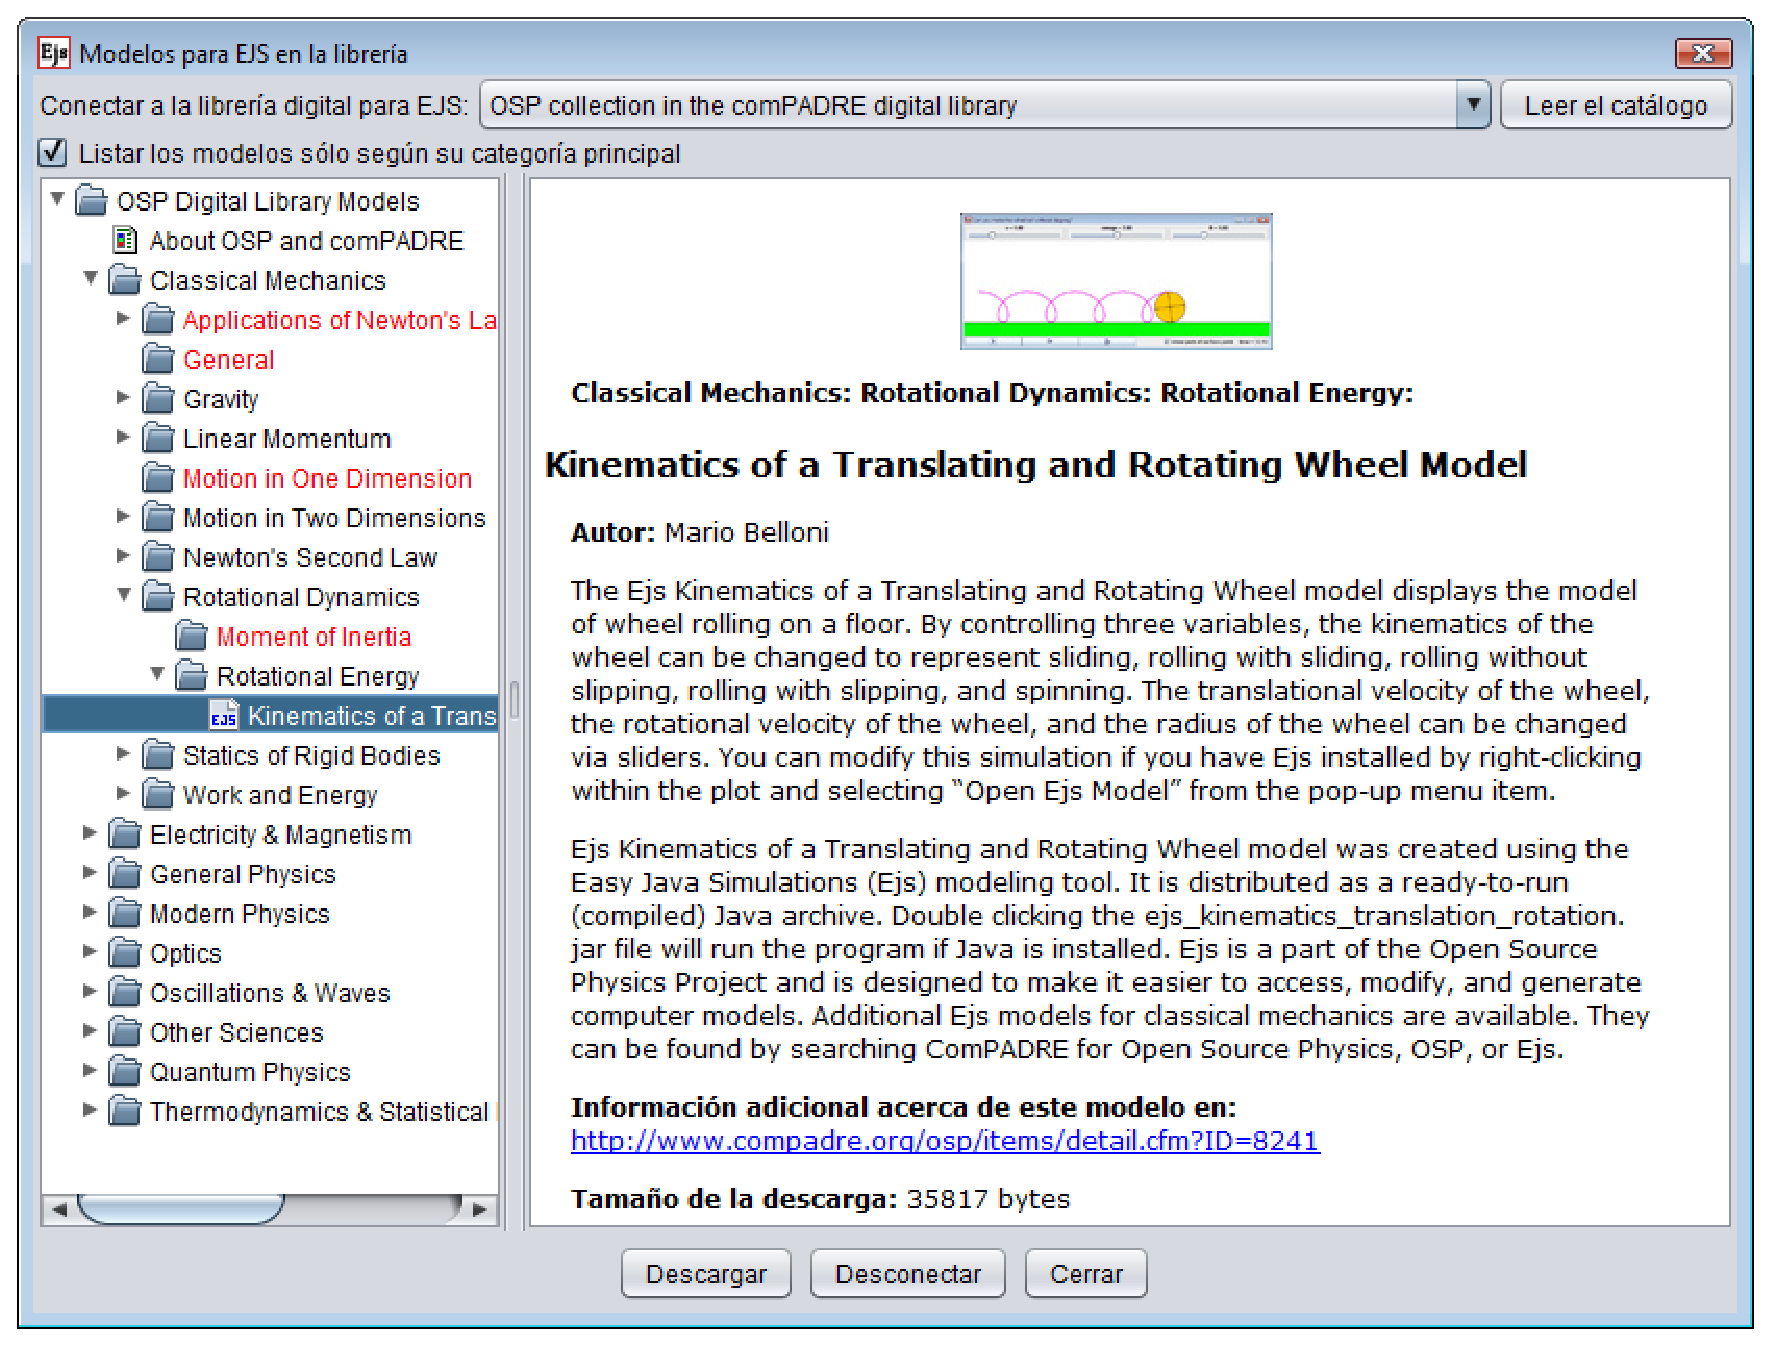
\includegraphics[scale=\scale]{02EjsIntro/images/OSPCollection.eps}
    \caption{La colecci�n OSP en la librer�a digital comPADRE. La colecci�n est� organizada en categor�as y subcategor�as. El nodo para un modelo proporciona informaci�n sobre el mismo.}
    \label{fig:02EjsIntro/OSPCollection}
\end{figure}

Cuando hace clic en el nodo de un modelo, el marco de la derecha muestra informaci�n sobre dicho modelo obtenida de manera instant�nea desde la librer�a. La informaci�n describe el modelo e incluye un enlace directo a la librer�a comPADRE para informaci�n adicional. Al hacer doble-clic en el nodo de un modelo, o al pulsar el bot�n \lit{Descargar}, \ejs\ obtiene los archivos del modelo y auxiliares desde la librer�a, le solicita un destino en el directorio \file{source} de su espacio de trabajo para descargarlos, y abre el modelo en \ejs\ cuando se completa la descarga. Como los ficheros fuente son t�picamente peque�os, la descarga tiene lugar casi instant�neamente. Ya puede inspeccionar, ejecutar o modificar el modelo de la misma forma que hicimos anteriormente en este mismo cap�tulo para el modelo de la masa y el muelle.

La colecci�n OSP de la librer�a digital comPADRE es un lugar altamente recomendado (si puede leer en ingl�s) para buscar modelos de \ejs\ y material curricular de acompa�amiento. Nosotros incluiremos a menudo referencias a la librer�a digital comPADRE en este libro, siempre que est�n relacionadas con lo descrito en el texto.

% -----------------------------------------------------
\section{Resumen}\label{section:02Review}
% -----------------------------------------------------

Este libro trata sobre el modelado y el uso de modelos para estudiar y visualizar un amplio rango de fen�menos, desde los m�s simples a los m�s complejos. Una forma adecuada de llevar a cabo este estudio es a trav�s de simulaciones por ordenador, �sto es, usar un ordenador para obtener datos num�ricos a partir de nuestros modelos conforme se desarrollan con el tiempo, y mostrar estos datos de forma que sean entendibles.

\Ejs\ es una herramienta de modelado y de autor expresamente dedicada a esta tarea. Ha sido dise�ado para permitirnos trabajar a un alto nivel conceptual, concentrando la mayor�a de nuestro tiempo y esfuerzo en los aspectos cient�ficos de la simulaci�n y pidiendo al ordenador que realice autom�ticamente todas aquellas tareas necesarias pero f�cilmente automatizables.
Toda herramienta, incluida \ejs, tiene una curva de aprendizaje. La primera parte del libro contiene una serie de ejemplos detallados para que se familiarice con las posibilidades de modelado de \ejs\ y con los elementos para la vista que se usan con mayor frecuencia. La segunda parte de este libro est� dedicada a ejemplos m�s avanzados y enfatiza el contenido cient�fico de los modelos y su comportamiento. Los ap�ndices cubrir�n cuestiones adicionales, como una revisi�n de Java y una serie de pautas que le ayudar�n en el inevitable momento en que cometa sus primeros errores de programaci�n.

Modelar es tanto una ciencia como un arte. Este libro le proporciona un s�lido punto de partida en la parte cient�fica, un repaso a las t�cnicas requeridas por el arte y ejemplos que son �tiles en la pr�ctica.

% -----------------------------------------------------
\section{Problemas y Proyectos}\label{section:02Projects}
% -----------------------------------------------------

%\subsection*{Problem 1}
\begin{problem}[Energ�a]
A�ada un tercer panel con ejes a la ventana de di�logo de la simulaci�n \file{Masa y muelle completo.xml} que muestre la evoluci�n de las energ�as cin�tica, potencial y total.
\end{problem}

%\subsection*{Problem 2}
\begin{problem}[Trazador de funciones]
La soluci�n anal�tica para un oscilador arm�nico simple sin rozamiento es
\begin{equation}
  x(t)=A \sin(w_0 t + \phi)
\end{equation}
donde $A$ es la amplitud (m�ximo desplazamiento), $w_0= \sqrt{k/m}$ es la frecuencia natural de la oscilaci�n y $\phi$ es el �ngulo de fase. Consulte un libro de mec�nica para encontrar la relaci�n entre la amplitud y el �ngulo de fase y el desplazamiento y velocidad iniciales. Utilice la simulaci�n \file{TrazadorDeFunciones.xml} del directorio de este cap�tulo para comparar la soluci�n anal�tica con la soluci�n num�rica generada por el modelo \file{MasaYMuelleCompleto.xml}.
\end{problem}

%\subsection*{Project 2}
\begin{project}[Oscilador en dos dimensiones]
Modifique el modelo de simulaci�n para masa y muelle para considerar un movimiento que no est� restringido a la direcci�n horizontal. Asuma que un segundo muelle con constante $k'$ produce una fuerza restauradora vertical $F_y(\delta y) = - k' \,\delta y$. Modifique la simulaci�n para permitir al usuario especificar las constantes de la ley de Hooke, y las condiciones iniciales en ambas direcciones. Describa el movimiento que se produce sin fuerza de rozamiento pero bajo diferentes condiciones iniciales y con distintas constantes para los muelles. (Pruebe $k=1$ y $k'=9$.) Muestre que es posible conseguir un movimiento circular haciendo $k=k'$.
\end{project}

%\subsection*{Project 3}
\begin{project}[P�ndulo simple]
Cree una simulaci�n parecida a la que se describe en este cap�tulo para un p�ndulo simple cuyo movimiento se describe mediante la ecuaci�n diferencial de segundo orden
\begin{equation}
  \frac{d^2\theta}{dt^2} = -\frac{g}{\ell} \sin (\theta),
\end{equation}
donde $\theta$ es el �ngulo del p�ndulo respecto de la vertical, $g$ es la aceleraci�n debida a la gravedad y $\ell$ es la longitud del hilo. Utilice relaciones fijas para calcular la posici�n $x$ e $y$ de la masa puntual del p�ndulo utilizando las ecuaciones:
\begin{align*}
   x   &=  \ell \, \sin (\theta) \\
   y   &= -\ell \, \cos (\theta).
\end{align*}
\end{project}
          % Chapter: Introduction to Ejs
      \include{Basics/mainBasics}                % Chapter: Ejs and Java basic concepts
      \include{Drawing/mainDrawing}              % Chapter: 2D and 3D drawing
      \include{04ODE/mainODE}                    % Chapter: Introduction to ODEs
      %\include{04ODE_WC/mainODE}
      \include{03Explicit/mainExplicit}          % Chapter: Explicit evolution algorithms
      % !TEX root = ../Guide de l'utilisateur de EjsS.tex

\chapter{Adding ``Events'' in \Ejs}\label{chapter:JavascriptEJS}
\begin{center} 
\copyright~\emph{July 2011 by Larry Engelhardt} \\{\small Adapted and edited by Francisco Esquembre}
\end{center}

This document provides a description of ``events'' in EJS---both what they are and how they are added.

\section{What is the purpose of an ``event'' in EJS?}

The purpose of an ``event'' is to provide a way for a certain \emph{action} to occur (for example, pausing the simulation) at the exact instant that a certain \emph{condition} is met (for example, a ball hitting the ground).  For the example of a falling ball, the following lines of code can be used to implement the Euler algorithm: 
\begin{verbatim}[8]
y = y + v*dt; // Update the height, y (using the velocity)
v = v + a*dt; // Update the velocity, v (using the acceleration)
t = t + dt;   // Update the time, t (using the time step, dt)
\end{verbatim}

For the example of a ball \emph{hitting the ground}, the ``event'' is analogous to the following lines of code:
\begin{verbatim}[8]
if (y < 0)  // If the condition is true...
{           // then the code within {...} is executed
  _pause(); // This pauses the simulation.
}
\end{verbatim}

Note these lines of code pause this simulation when the ball hits the ground. (More precisely, this pauses the simulation \emph{after} the ball hits the ground.)  Using an event will accomplish the same purpose, but the use of an event will be superior to these lines of code in two ways:
\begin{enumerate}
\item The event will be more accurate than this code.
\item The event will be even simpler to create than this code.
\end{enumerate}

Using an event will be more \emph{accurate} than the lines of code listed above for the following reason.  The lines of code above are only executed at the discrete time steps $t=0$, $\Delta t$, $2\Delta t$, $3\Delta t$, $4\Delta t$, etc.  When using an event, EJS does much better than this.  If the height is found to change from a positive value to a negative value between $t=2\Delta t$ and $t=3\Delta t$, the ODEs will be re-evaluated (meaning that the height will be re-evaluated) at $t=2.5\Delta t$ (midway between the two times).  This will hence provide a better approximation to the \emph{actual} time that the ball hits the ground.  This process will then be repeated.  If the height is found to change from positive to negative between $t=2\Delta t$ and $t=2.5\Delta t$, the ODEs will be re-evaluated at $t=2.25\Delta t$ (the new midway point between the times). The number of times that this process is repeated is referred to as the number of \emph{iterations}, and since each iteration involves cutting the time interval in half, this method is referred to as the \emph{bisection} method.  After several iterations, this process should give a very accurate approximation to the exact moment that the event occurs.  (This process of finding precisely where a function crosses zero is generally referred to as \emph{root finding}.)

\section{How are events added in EJS?}

Creating an event in EJS is also very \emph{simple} to do. After creating a page of ODEs, an event can be added by clicking on the button labeled ``Events''.  After creating an event, a window will appear. This window is shown in Fig.~\ref{fig:appendixA/Events}.


\begin{figure}[htb]
  \centering
  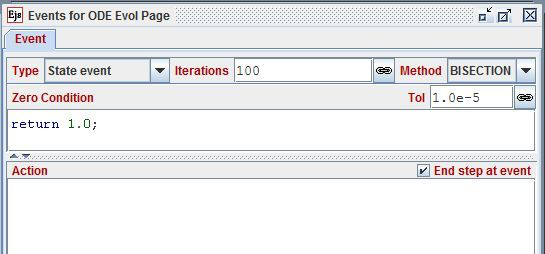
\includegraphics[scale=\scale]{appendixA/images/events_image.png}
  \caption{The blank page that appears when adding an event.}
  \label{fig:appendixA/Events}
\end{figure}

At the top of the window shown in Fig.~\ref{fig:events} several options can be specified. The menu in the top left corner allows you to choose the ``type'' of event to be used, as described in the following section. The maximum number of iterations (described in the previous section) can also be specified at the top of the page.  In the top right corner, the method of iteration can be selected.  The bisection method is described in the previous section.  The secant method is similar, but uses a secant line between the two points in time to estimate when the crossing event occurs.

Finally, it is necessary to specify the ``Zero condition'' and the ``Action''.  The zero condition consists of one or more lines of code, and it must include a \verb return ~statement. The quantity (or the \underline{\textbf{variable}}) following the word ``return'' will be checked to see whether or not the event has occurred (e.g., whether or not the ball has hit the ground).  For example, with the statement \verb+return 1.0;+ the event will never occur because 1.0 will always be greater than zero!  In fact, you would \emph{never} want to return a fixed numerical value because a fixed value can never change sign.  Hence, you need to replace the ``1.0'' with the thing that \emph{does} cross zero (and does change sign) at the moment that the event should occur.  One of the keys to using an event is to decide what quantity should follow the word \verb+return+.  The ``Action'' is the code to be executed when the event occurs, and it needs to be entered into the lower part of the window.

For the example of a ball hitting the ground, the \emph{event} can be described as ``the moment that the height crosses the value $y=0$''.  Hence, the \verb return ~statement would be \verb+return y;+.  This completed event is shown in Fig.~\ref{fig:appendixA/EventsComplete}.

\begin{figure}[htb]
  \centering
  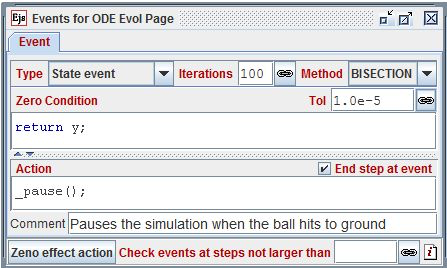
\includegraphics[scale=\scale]{appendixA/images/event_complete.png}
  \caption{The completed event that will pause the simulation when an object hits the ground.}
  \label{fig:appendixA/EventsComplete}
\end{figure}

\newpage
\section{Different ``types'' of events}

In the upper-left corner of the Event window (visible in Figs.~\ref{fig:events}~and~\ref{fig:events_complete}), you are able to choose between three different ``types'' of events:
\begin{enumerate}
\item State event
\item Zero crossing
\item Positive crossing
\end{enumerate}

Specifying the ``type'' of event to use can be a bit confusing for the following reason:  Your choice of which type of event to use \emph{doesn't matter}\ldots unless it does!  For example, the event shown in Fig.~\ref{fig:events_complete} that pauses the falling ball will work correctly regardless of which type of event is used.  In other situations though, the correct choice of event type can be very important.

Let us first consider the ``Zero crossing'' event.  This does exactly what you would expect.  When the value of the quantity specified by the \verb+return+ statement crosses zero, the event is triggered, and the \emph{Action} is executed.  The ``Positive crossing'' event does the same thing, except this type of event is \emph{only} triggered when the value of the quantity changes from positive to negative---not negative to positive.  Clearly either of these would work for the falling object, since---at the moment that it hits the ground---the height crosses zero \emph{and} changes sign from positive to negative.  As a different example, when using an event to measure the period of some type of oscillation, you might wish to use a \emph{positive} crossing rather than a \emph{zero} crossing.  This would allow you to measure the \emph{complete} period rather than only half an oscillation.  You might wonder why there is not a corresponding ``Negative crossing''.  Detecting a negative crossing is a very reasonable thing to want to do, and it is very easily accomplished:  Simply use a positive crossing, and include a negative sign after the word \verb+return+ in the Zero Condition!

The ``State event'' is just like the ``Positive crossing'' event, except that a \emph{state} event should be used in situations where it is \emph{not allowed} for the value of the quantity to be negative.  Examples could include objects \emph{bouncing} off of the ground, or off of a wall, or off of each other.  In these situations, you are \emph{required} to include code within the Action that will keep the quantity (following the \verb+return+) out of the ``forbidden region''.  For the examples of bouncing objects, this is accomplished by simply changing the sign of the velocities within the action.  For a concrete example of the difference between state events and positive crossing events, do the following:
\begin{enumerate}
\item Open the Event window shown in Fig.~\ref{fig:events_complete}, and remove (or comment out) the line of code that appears in the Action.  (Now the program will continue after the event is triggered.)
\item Run the program with \emph{State event} selected for the event type.  With a state event, negative values are not allowed, so you will see an error.  (This is EJS politely tapping you on the shoulder to let you know that you are ``breaking the rules''.)
\item Run the program again with either \emph{Zero crossing} or \emph{Positive crossing} selected for the event type.  Now there is no error, since negative values \emph{are} allowed for these types of events.
\end{enumerate}

As a final example, again select ``State event,'' but now specify \verb+v = -0.9*v;+ for the Action.  This will make the ball \emph{bounce}; but since the coefficient of restitution is less than 1, the maximum height of the ball will decrease (by the \emph{same fraction}) with each bounce.  We could now ask the question, ``How long will it take for the ball to come to rest?'' which is reminiscent of \emph{Zeno's paradoxes}.  To address these situations, click on the ``Zeno effect action'' button shown in the lower-left corner of Fig.~\ref{fig:events_complete}, and enter additional code to be executed in the event of infinitesimal bounces---e.g., pausing or resetting the simulation.



              % Chapter: Events
     \include{06Systems/mainSystems}            % Chapter: Systems of particles
    \part{From Free Fall to Chaos} %Focus on the science.
      \include{06Oscillation/mainOscillation} % Chapter: Oscillations and analysis tools/techniques
      \include{07Chaos/mainChaos}     % Chapter: The chaotic motion of Dynamical Systems
      \include{08Orbits/mainOrbits} % Chapter: Planetary motion
      \include{09Geometry/mainGeometry}   % Chapter: Geometry, quaternions, and rigid body motion
      \include{10PDE/mainPDE}         % Chapter: Partial differential equations
      \include{12Self/mainSelf}       % Chapter: Self-organized systems
      \include{13Biology/mainBiology} % Chapter: Biological Systems
      \include{14Social/mainSocial}   % Chapter: Social Science Systems

    \appendix
      \include{appendixA/mainDistribution} % Appendix: Distribution of Ejs models as Launcher packages
      % !TEX root = ../EjsS Manual.tex

\chapter{Exploring the Java flavor of \Ejs}\label{chapter:JavaEJS}

\begin{quote}
A good example is the best sermon.  {\em Benjamin Franklin}
\end{quote}

To  provide a perspective of the modeling process, in this chapter we first load, inspect, and run an existing simple harmonic oscillator simulation. We then modify the simulation to show how \ejs\ engages the user in the modeling process and greatly reduces the amount of
programming that is required. This chapter uses Java as the programming language for the modeling and is a twin chapter of Chapter~\ref{chapter:JavascriptEJS} (where Javascript is used).

% ------------------------
    \section{Inspecting the Simulation}\label{section:02ExplorationJavaInspecting}\index{\Ejs!inspecting a simulation}
% ------------------------

As mentioned in Chapter~\ref{chapter:EjsIntro}, \Ejs\ provides three workpanels for modeling. The first panel, \lit{Description}, allows us to create and edit multimedia HTML-based narrative that describes the model.\index{HTML} 
The second work panel, \lit{Model}, is dedicated to the modeling process. We use this panel to create
variables that describe the model, to initialize these variables, and to write algorithms that describe how this model
changes in time. The third workpanel, \lit{View}, is dedicated to the task of building the graphical user interface,
which allows users to control the simulation and to display its output.  

To understand how the \lit{Description}, \lit{Model}, and \lit{View} workpanels work together, we inspect and run an
already existing simulation. Screen shots are no substitute for a live demonstration, and you are encouraged to follow along on your computer as you read.

\begin{figure}[htb]
  \centering
  \subfigure{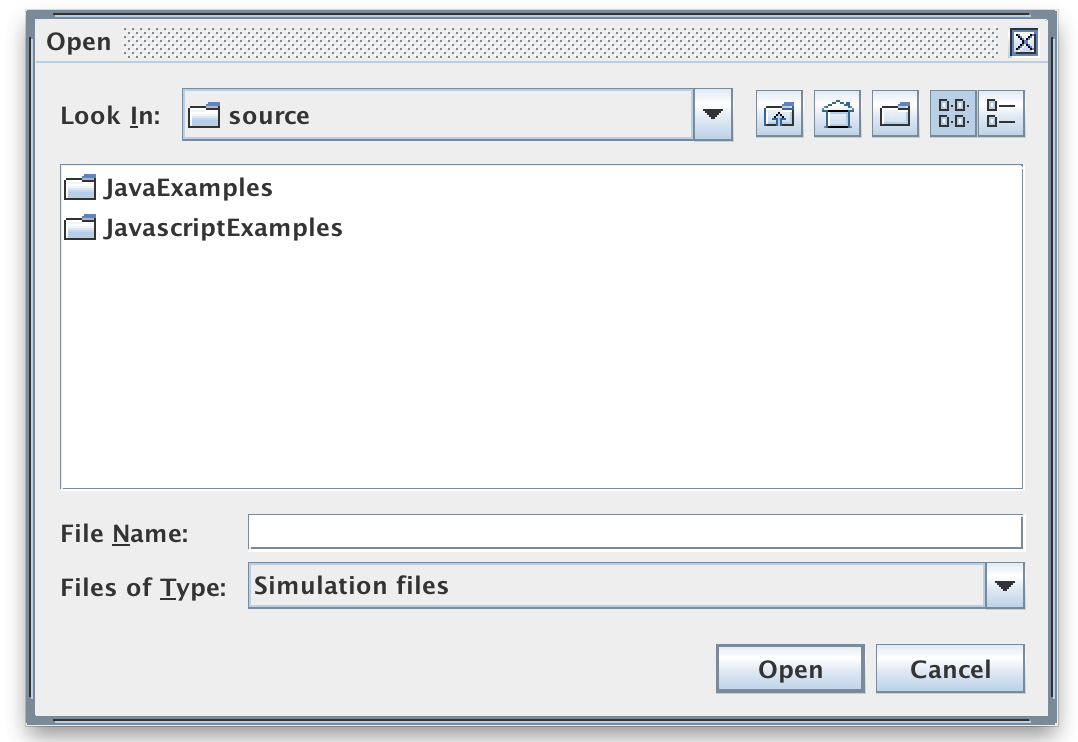
\includegraphics[scale=0.2]{02ExplorationJava/images/OpenDialogCrossPlatform.png}}
  \subfigure{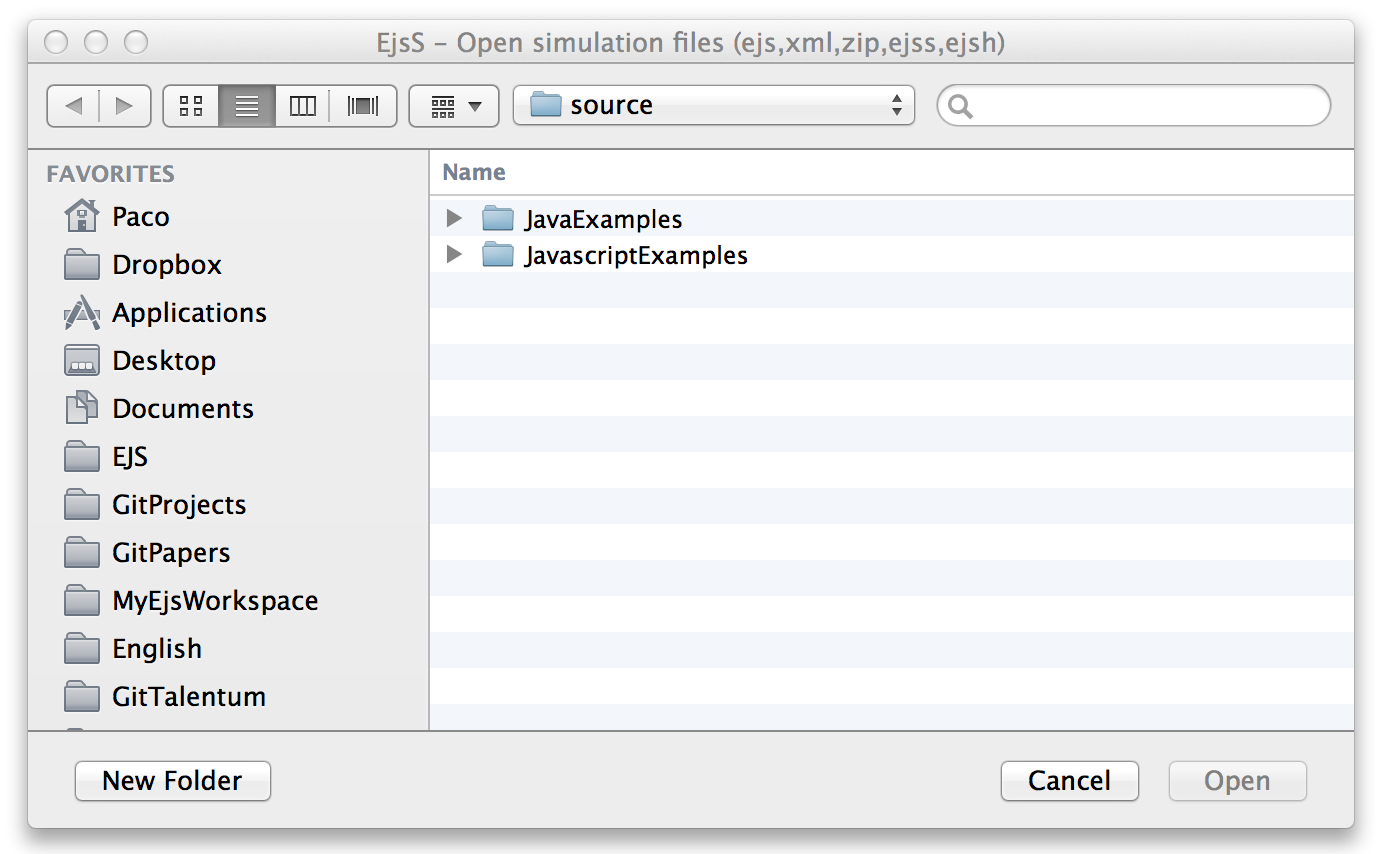
\includegraphics[scale=0.2]{02ExplorationJava/images/OpenDialogNative.png}}  
  \caption{The open file dialog lets you browse your hard disk and load an existing simulation. The appearance of the dialog 
  (shown here using two different look and feels) may vary, depending on your operating system and the selected \lit{look and feel}.}
  \label{fig:02ExplorationJava/OpenDialog}
\end{figure}

Click on the \lit{Open} icon 
\includegraphics[scale=\linescale]{../_common/icons_png/openSmall.png} on the \ejs\ taskbar. A file dialog
similar to that in Figure~\ref{fig:02ExplorationJava/OpenDialog} appears showing the contents of your workspace's \file{source}
directory. Go to the \file{JavaExamples} directory, where you will find a
file called \file{MassAndSpring.ejs}. Select this file and click on the \lit{Open} button of the
file dialog.

Now, things come to life! \ejs\ reads the \file{MassAndSpring.ejs} document which populates the workpanels and two new
``Ejs windows'' appear in your display as shown in Figure~\ref{fig:02ExplorationJava/SpringInterface}. A quick warning. You
can drag objects within these mock-up windows but this will set the model's initial conditions.  It is usually better
to set initial conditions using a table of variables as described in Section~\ref{section:02ExplorationJavaModel}.

\begin{figure}[htb]
  \centering
  \subfigure{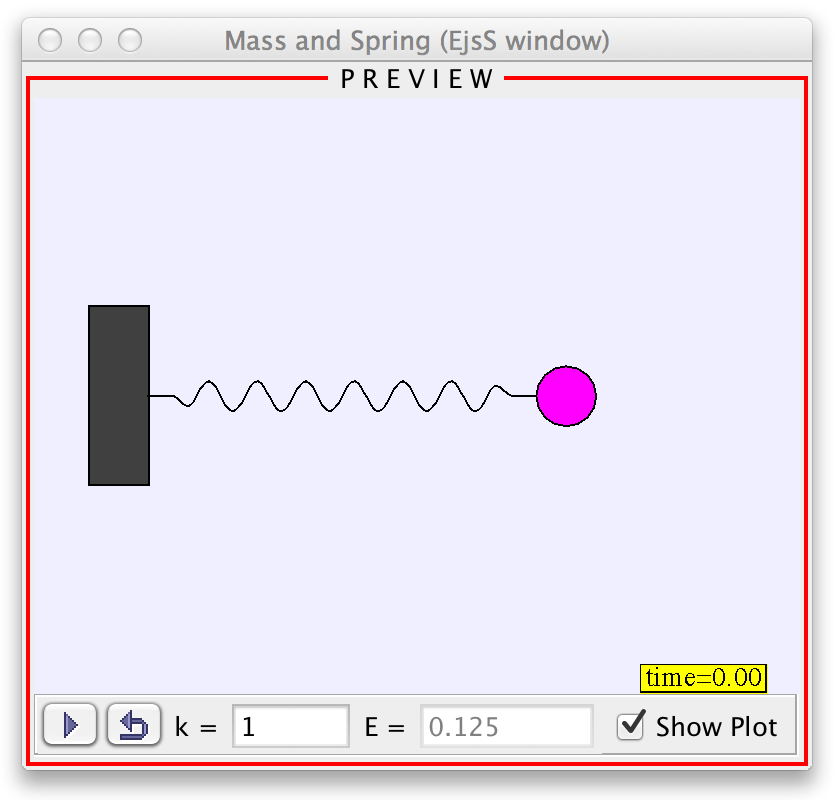
\includegraphics[scale=\scale]{02ExplorationJava/images/SpringInterface1.png}}
  \subfigure{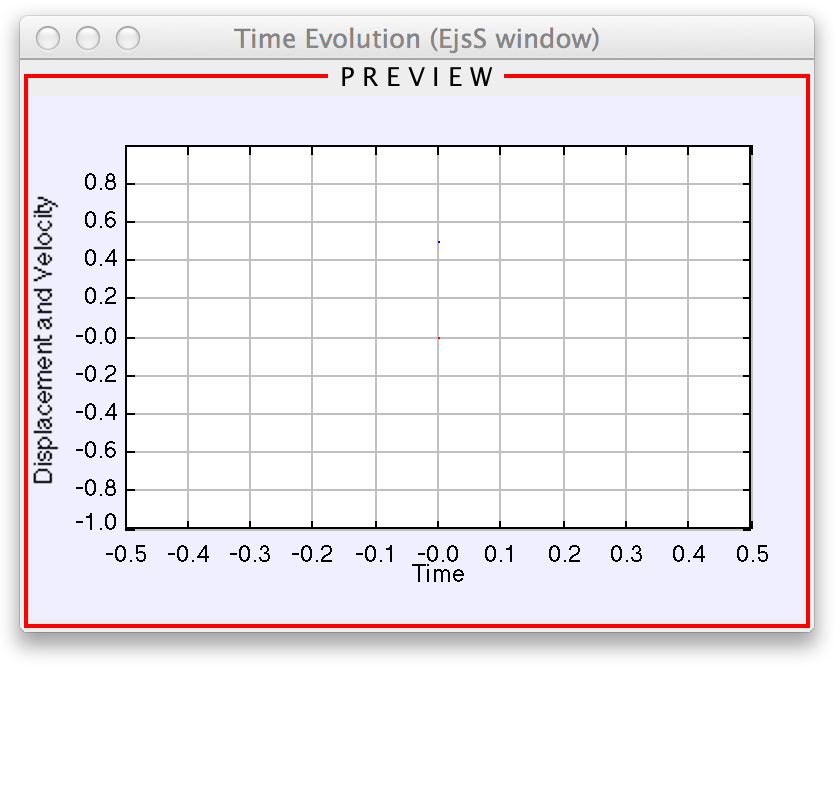
\includegraphics[scale=\scale]{02ExplorationJava/images/SpringInterface2.png}}
  \caption{\ejs\ mock-up windows of the \file{MassAndSpring} simulation. The title bar and the red border show that they are \ejs' windows
  and that the program is not running.}
  \label{fig:02ExplorationJava/SpringInterface}
\end{figure}

\note{Impatient or precocious readers may be tempted to click on the green run icon \includegraphics[scale=\linescale]{../_common/icons_png/launch.png} on the taskbar to execute our
example before proceeding with this tutorial.  Readers who do so will no longer be interacting with \ejs\  but with a compiled and running Java program.  Exit the running program by closing the \lit{Mass and Spring} window or by right clicking on the (now) red-squared stop icon \includegraphics[scale=\linescale]{../_common/icons_png/stop.png} on \ejs' taskbar before proceeding.}

\subsection{The \lit{Description} workpanel}

Select the \lit{Description}\index{Ejs!Description} workpanel by clicking on the corresponding radio button at the top of
\ejs, and you will see two pages of narrative for this simulation. The first page, shown in
Figure~\ref{fig:02ExplorationJava/SpringDesc}, contains a short discussion of the mass and spring model. Click on the
\lit{Activities} tab to view the second page of narrative.

\begin{figure}[htb]
  \centering
  \includegraphics[scale=\scale]{02ExplorationJava/images/SpringDesc.png}
  \caption{The description pages for the mass and spring simulation. Click on a tab to display the page. Right-click on a tab to edit the page.}
  \label{fig:02ExplorationJava/SpringDesc}
\end{figure}

A \lit{Description} is HTML\index{HTML} or XHTML\index{XHTML} multimedia text that provides information and instructions about the
simulation. HTML stands for HyperText Markup Language and is the most commonly used protocol for formatting and
displaying documents on the Web. The X in XHTML stands for eXtensible. XHTML is basically HTML expressed as valid XML or, in simpler words, perfectly formatted HTML.

\ejs\ provides a simple HTML editor that lets you create and modify pages within \ejs.
You can also import HTML or (preferably) XHTML pages into \ejs\ by right clicking on a tab in the \lit{Description} workpanel. (See
Section~\ref{section:02ExplorationJavaModifyingDescription}.) Description pages are an essential part of the modeling process and
these pages are included with the compiled model when the model is exported for distribution.

\subsection{The \lit{Model} workpanel}\label{section:02ExplorationJavaModel}

The \lit{Model} workpanel is where the model is defined so that it can be converted into a program by \ejs. In this simulation,
we study the motion of a particle of mass $m$ attached to one end of a massless spring of equilibrium length $L$.
The spring is fixed to the wall at its other end and is restricted to move in the horizontal direction. Although the
oscillating mass has a well known analytic solution, it is useful to start with a simple harmonic oscillator model so that
our output can be compared with an exact analytic result.\index{Simple Harmonic Motion}

Our model assumes small oscillations so that the spring responds to a given (horizontal) displacement $\delta x$ from
its equilibrium length $L$ with a force given by Hooke's law,\index{Hooke's law} $F_x = - k \,\delta x$, where $k$ is
the elastic constant of the spring, which depends on its physical characteristics. We use Newton's second
law\index{Newton's second law} to obtain a second-order differential equation for the position of the particle:
\begin{equation}
  \frac{d^2\ x}{dt^2} = -\frac{k}{m}\,(x-L). \label{eq:02ExplorationJava/SpringBasic}
\end{equation}
Notice that we use a system of coordinates with its $x$-axis along the spring and with its origin at the
spring's fixed end. The particle is located at $x$ and its displacement from equilibrium $\delta x=x-L$ is zero when $x=L$. We solve this system numerically to study how the state evolves in time.

Let's examine how we implement the mass and spring model by selecting the \lit{Model} radio button and examining each of
its six panels.

\subsubsection{Declaration of variables}
\begin{figure}[htb]
    \centering
  \includegraphics[scale=\scale]{02ExplorationJava/images/ModelVariables.png}
    \caption{The \lit{Model} workpanel contains six subpanels. The subpanel for the definition of mass and spring dynamical variables is displayed.  Other tabs in this subpanel define additional variables, such as the natural length of the spring $L$ and the energy $E$.} \label{fig:02ExplorationJava/ModelVariables}
\end{figure}

When implementing a model, a good first step is to identify, define, and initialize the variables that describe the
system. The term \emph{variable} is very general and refers to anything that can be given a name, including a
physical constant and a graph\index{Model!Variables}. Figure~\ref{fig:02ExplorationJava/ModelVariables} shows an
\ejs\ variable table. Each row defines a variable of the model by specifying the name of the variable, its type, its dimension, and its initial value.

Variables in computer programs can be of several types depending on the data they hold. The most frequently used types are \code{boolean} for true/false values, \code{int} for integers, \code{double} for high-precision ($\approx 16$ significant digits) numbers, and \code{String} for text.  We will use all these variable types in this document, but the mass and spring model uses only variables of type \code{double} and \code{boolean}.

Variables can be used as parameters, \index{Model!Parameters} state variables,\index{Model!State variables} or inputs and outputs of the model.\index{Model!Input and Output}  The tables in Figure~\ref{fig:02ExplorationJava/ModelVariables} define the variables used within our model.  We have
declared a variable for the $x$-position of the particle, \code{x}, for its velocity in the
$x$-direction, \code{vx}, for the time, \code{t}, and for the increment of time at each simulation step, \code{dt}.
We define some variables, in this and other tabs, that do not appear in Equation\eqref{eq:02ExplorationJava/SpringBasic}. The reason for auxiliary variables, such as  \code{vx} or the kinetic, potential, and total energies, will be made clear in what follows. The bottom part of the variables panel contains a comment field that provide a description of the role of each variable in the model. Clicking on a variable displays the corresponding comment.

\subsubsection{Initialization of the model}
Correctly setting initial conditions is important when implementing a model because the model must start in a
physically realizable state. Our model is relatively simple, and we initialize it by entering values (or simple Java
expressions such as \code{0.5*m*vx*vx}) in the \lit{Initial value} column of the table of variables. \ejs\ uses these values when it initializes the simulation.

\note{Advanced models may require an initialization algorithm. For example, a molecular dynamics model may set particle
velocities for an ensemble of particles. The \lit{Initialization} panel allows us to define one or more pages of Java
code that perform the required computation. \ejs\ converts this code into a Java method\index{Java!method}\footnote{A
Java method is similar to a function or a subroutine in procedural computer languages.} and calls this method at
start-up and whenever the simulation is reset. The mass and spring \lit{Initialization} panel is not shown here because
it is empty. See Subsection~\ref{section:02ExplorationJavaInspectingRelations} for an example of how Java code appears in \ejs.}

\subsubsection{The evolution of the model}

The \lit{Evolution} panel allows us to write the Java code that determines how the mass and spring system evolves in time and we will use this option frequently for models not based on ordinary differential equations (ODEs). There is, however, a second option that allows us to enter ordinary differential equations, such as \eqref{eq:02ExplorationJava/SpringBasic}, without programming.  \ejs\ provides a dedicated editor that lets us specify differential equations in a format that resembles mathematical
notation and automatically generates the correct Java code.

Let's see how the differential equation editor works for the mass and spring model. Because ODE algorithms solve
systems of first-order ordinary differential equations, a higher-order equation, such as
\eqref{eq:02ExplorationJava/SpringBasic}, must be recast into a first-order system.   We can do so by treating the
velocity as an independent variable which obeys its own equation:
\begin{align}
  \frac{d\ x} {dt} &= v_x                           \label{eq:02ExplorationJava/SpringBasicODE1} \\
  \frac{d\ v_x}{dt} &= -\frac{k}{m}\,(x-L). \label{eq:02ExplorationJava/SpringBasicODE2}
\end{align}
The need for an additional differential equation explains why we declared the \code{vx} variable in our table of
variables.

Clicking on the \lit{Evolution} panel displays the ODE editor shown in
Figure~\ref{fig:02ExplorationJava/ModelEvolution}.
\begin{figure}[htb]
    \centering
  \includegraphics[scale=\scale]{02ExplorationJava/images/ModelEvolution.png}
    \caption{The ODE evolution panel showing the mass and spring differential equation and the numerical algorithm.}
    \label{fig:02ExplorationJava/ModelEvolution}
\end{figure}
Notice that the ODE editor displays \eqref{eq:02ExplorationJava/SpringBasicODE1} and \eqref{eq:02ExplorationJava/SpringBasicODE2}
(using the  \lit{*} character to denote multiplication). Fields near the top of the editor specify the independent variable
\code{t} and the variable increment \code{dt}.  Numerical algorithms approximate the exact ODE solution by advancing
the state in discrete steps and the increment determines this step size.
The \lit{Prelim code} button at the top-right of the editor allows us to enter preliminary code, to perform computations prior to evaluating the equations (a circumstance required in more complex situations than the one we treat in this example). A dropdown menu at the bottom of the editor
lets us select the ODE solver (numerical algorithm) that advances the solution from the current value of time, \code{t}, to the next value, \code{t + dt}. The tolerance field (\lit{Tol}) is greyed out and empty because Euler--Richardson is a fixed-step method that requires no tolerance settings. The advanced button displays a dialog which allows us to fine-tune the execution of this solver, though default values are usually appropriated. Finally, the events field at the bottom of the panel tells us that we have not defined any events for this differential equation. Examples with preliminary code and events can be found further on in this document. The different solver algorithms and its parameters are discussed in the \ejs\ help.

The left-hand side of the evolution workpanel includes fields that determine how smoothly and how fast the simulation runs.
The \lit{frames per second} (\lit{FPS}) option, which can be selected by using either a slider or an input field,
specifies how many times per second we want our simulation to repaint the screen. The \lit{steps per display}
(\lit{SPD}) input field specifies how many times we want to advance (step) the model before repainting. The current
value of \code{20} frames per second produces a smooth animation that, together with the prescribed value of one step
per display and \code{0.05} for \code{dt}, results in a simulation which runs  at (approximately) real time. We will
almost always use the default setting of one step per display. However, there are situations where the model's
graphical output consumes a significant amount of processing power and where we want to speed the numerical
computations. In this case we can increase the value of the steps per display parameter so that the model is advanced
multiple times before the visualization is redrawn. The \lit{Autoplay} check box indicates whether the simulation
should start when the program begins. This box is unchecked so that we can change the initial conditions before
starting the evolution.

The evolution workpanel handles the technical aspects of the mass and spring ODE model without programming.  The
simulation advances the state of the system by numerically solving the model's differential equations using the
midpoint algorithm. The algorithm steps from the current state at time \code{t} to a new state at a new time
\code{t + dt} before the visualization is redrawn. The simulation repeats this evolution step \code{20} times per second
on computers with modest processing power. The simulation may run slower and not as smoothly on computers with
insufficient processing power or if the computer is otherwise engaged, but it should not fail.

\note{Although the mass and spring model can be solved with a simple ODE algorithm, our numerical methods library
contains very sophisticated algorithms and \ejs\ can apply these algorithms to large systems of vector differential
equations with or without discontinuous events.}

\subsubsection{Relations among variables}\label{section:02ExplorationJavaInspectingRelations}
Not all variables within a model are computed using an algorithm on the Evolution workpanel. Variables can also be computed after the evolution has been applied. We refer to variables that are computed using the evolution algorithm as state variables or dynamical variables, and we refer to variables that depend on these variables as auxiliary or output variables. In the mass and
spring model the kinetic, potential, and total energies of the system are output variables because they are computed
from state variables.
\begin{align}
  T &= \frac{1}{2} m {v_x}^2,     \label{eq:02ExplorationJava/SpringEnergy1} \\
  V &= \frac{1}{2} k (x-L)^2,     \label{eq:02ExplorationJava/SpringEnergy2} \\
  E &= T + V.                     \label{eq:02ExplorationJava/SpringEnergy3}
\end{align}
We  say that there exists \emph{fixed relations} among the model's variables.

The \lit{Fixed relations} panel shown in Figure~\ref{fig:02ExplorationJava/ModelRelations} is used to write relations among
variables. Notice how easy it is to convert \eqref{eq:02ExplorationJava/SpringEnergy1} through
\eqref{eq:02ExplorationJava/SpringEnergy3} into Java syntax. Be sure to
use the multiplication character \lit{*} and to place a semicolon at the end of each Java statement.

\begin{figure}[htb]
    \centering
  \includegraphics[scale=\scale]{02ExplorationJava/images/ModelConstraints.png}
    \caption{Fixed relations for the mass and spring model.}
    \label{fig:02ExplorationJava/ModelRelations}
\end{figure}

\noindent \textbf{Here goes an important remark.} You may wonder why we do not write fixed relation expressions by adding a second code page after the ODE page in the
\lit{Evolution} panel. After all, evolution pages execute sequentially and a second evolution page would correctly
update the output variables after every step. The reason that the \lit{Evolution} panel should not be used is that
relations must \emph{always} hold and there are other ways, such as mouse actions, to affect state
variables. For example, dragging the mass changes the $x$ variable and this change affects the energy.
\ejs\ automatically evaluates the relations after initialization, after every evolution step, and whenever
there is any user interaction with the simulation's interface.  For this reason, it is important that fixed relations among variables be written in the \lit{Fixed relations} workpanel.

\subsubsection{Custom pages}

There is a fifth panel in the \lit{Model} workpanel labeled \lit{Custom}. This panel can be used to define Java methods (functions) that can be used throughout the model.  This panel is empty because our model currently doesn't require additional methods,
but we will make use of this panel when we modify our mass and spring example in Section~\ref{section:02ExplorationJavaModifying}.  A
custom method is not used unless it is explicitly invoked from another workpanel.

\subsubsection{Model elements}

The final, sixth panel in the \lit{Model} workpanel is labeled \lit{Elements} and provides access to third-party Java libraries in the form of drag and drop icons. You add these libraries to your program by dragging the corresponding icon to the list of model elements to use for this model. This creates Java objects you can then use in your model code. This panel is also empty for this model because our mass and spring doesn't require additional Java libraries.

% ---------------------------------------------
\subsection{The \lit{View} workpanel}
% ---------------------------------------------

The third \Ejs\ workpanel is the \lit{View}.  This workpanel allows us to create a graphical interface that includes
visualization, user interaction, and program control with minimum programming.
Figure~\ref{fig:02ExplorationJava/SpringInterface} shows the view for the mass and spring model. Select the \lit{View} radio
button to examine how this view is created.

The right frame of the view workpanel of \ejs, shown in Figure~\ref{fig:02ExplorationJava/View}, contains a collection of
\emph{view elements},\index{Ejs!view elements} grouped by functionality. View elements are building blocks that can be
combined to form a complete user interface, and each view element is a specialized object with an on-screen
representation. To display information about a given element, click on its icon and press the \lit{F1} key or right-click and select the \lit{Help} menu item. To create a user interface, we create a frame (window) and add elements, such as buttons and graphs, using ``drag and drop'' as described in Section~\ref{section:02ExplorationJavaModifying}.

\begin{figure}[htb]
    \centering
  \includegraphics[scale=\scale]{02ExplorationJava/images/View.png}
    \caption{The \lit{View} workpanel showing the \emph{Tree of elements} for the mass and spring user interface.}
    \label{fig:02ExplorationJava/View}
\end{figure}

The \emph{Tree of elements} shown on the left side of Figure~\ref{fig:02ExplorationJava/View} displays the structure of the
mass and spring user interface. Notice that the simulation has two windows, a \code{Frame} and a \code{Dialog}, that appear on your computer screen.
These elements belong to the class of \emph{container} elements whose primary
purpose is to visually group (organize) other elements within the user interface.
The tree displays descriptive names and icons for these elements.   Right-click on an element of the tree to
obtain a menu that helps the user change this structure. Alternatively, you can drag and drop elements from one container to another to change the parent-child relationship, or within a container to change the child order. (There are conditions for a container to accept a given element as child. For instance, a two-dimensional drawing panel can only accept 2D drawable elements.)

Each view element has a set of internal parameters, called \emph{properties},\index{Ejs!view element properties} which
configure the element's appearance and behavior. We can edit these properties by double clicking on the element in the
tree to display a table known as a \emph{properties inspector}.  Appearance properties, such as color, are often set to a constant value, such as \code{RED}. We can also use a variable from the model to set an element's property. This ability to connect (bind) a property to a variable without programming is the key to turning our view into a dynamic and interactive
visualization.

Let's see how this procedure works in practice. Double-click on the \code{massShape2D} element (the `Shape2D' suffix we added to the element's name helps you know the type of the element) in the tree to display
the element's properties inspector. This element is the mass that is attached at the free end of the spring. The massShape2D's table of properties appears as shown in Figure~\ref{fig:02ExplorationJava/SpringBallProperties}.
\begin{figure}[htb]
    \centering
  \includegraphics[scale=\scale]{02ExplorationJava/images/SpringBallProperties.png}
    \caption{The table of properties of the \code{massShape2D} element.}
    \label{fig:02ExplorationJava/SpringBallProperties}
\end{figure}

Notice the properties that are given constant values. The \code{Style}, \code{Size X}, \code{Size Y}, and \code{Fill
Color} properties produce an ellipse of size \code{(0.2,0.2)} units (which makes a circle) filled with the color
magenta. More importantly, the \code{Pos X} and \code{Pos Y} properties of  the shape are bound to the \code{x} and \code{y}
variables of the model. This simple assignment establishes a bidirectional connection between model and view. These
variables change as the model evolves and the shape follows the \code{x} and \code{y} values. If the user drags the
shape to a new location, the \code{x} and \code{y} variables in the model change accordingly.  Note that the \code{Draggable} property is only enabled when the animation is paused.

Elements can also have \emph{action properties}\index{Ejs!action properties} which can be associated with code.
(Action properties have their labels displayed in red.) User actions, such as dragging or clicking, invoke their
corresponding action property, thus providing a simple way to control the simulation. As the user drags the mass, the code on the \code{On Drag} property restricts the motion of the shape to the horizontal direction by setting the \code{y} variable to \code{0}.  Finally, when the mouse button is
released, the following code is executed:

\begin{listing}
\begin{verbatim}
vx = 0.0;            // sets the velocity to zero
_view.resetTraces(); // clears all plots
\end{verbatim}
\end{listing}

\noindent Clicking on the icon next to the field displays a small editor that shows this code.

\note{Because the \code{On Release} action code spans more than one line, the property field in the inspector shows a darker (green) background. Other data types, such as boolean properties, have different editors.  Clicking the second icon displays a dialog window with a listing of variables and methods that can be used to set the property value.}

\begin{exercise}[Element inspectors]\label{ex:02ExplorationJava/properties}
The mass' inspector displays different types of properties and their possible values. Explore the properties of other
elements of the view.  For instance, the \code{displacementTrail2D} and \code{velocityTrail2D} elements correspond to the
displacement and velocity time plots in the second window of the view, respectively.  What is the maximum number of points that can be added to each trail?
\end{exercise}

\subsection{The completed simulation}

We have seen that \Ejs\ is a powerful tool that lets us express our knowledge of a model at a very high level of abstraction. When modeling the mass and spring, we first created a table of variables that describes the model and initialized these variables using a column in the table. We then used an evolution panel with a high-level editor for systems of first-order ordinary differential equations to specify how the state advances in time. We then wrote relations to compute the auxiliary or output variables that can be expressed using expressions involving state variables.  Finally, the program's graphical user interface and high-level visualizations were created by dragging objects from the \lit{Elements} palette into the \lit{Tree of elements}. Element properties were set using a properties editor and some properties were associated with variables from the model.

It is important to note that the three lines of  code on the Fixed relations workpanel (Figure~\ref{fig:02ExplorationJava/ModelRelations}) and the two lines of code in the particle's action method are the only explicit Java code needed to implement the model.  \Ejs\ creates a complete Java program by processing the information in the workpanels when the run icon is pressed as described in Section~\ref{section:02ExplorationJavaRunning}.

% -----------------------------------------------------
\section{Running the Simulation}\label{section:02ExplorationJavaRunning}\index{Simulation!running}
% -----------------------------------------------------

It is time to run the simulation by clicking on the \lit{Run} icon of the taskbar, \includegraphics[scale=\linescale]{../_common/icons_png/launch.png}.  \ejs\ generates the Java code and compiles it, collects auxiliary and library files, and executes the compiled program. All at a single mouse click.

Running a simulation initializes its variables and executes the fixed relations to insure that the model is in a consistent state.  The model's time evolution starts when the play/pause button in the user interface is pressed. (The play/pause button displays the \includegraphics[scale=\linescale]{../_common/icons_png/play.png} icon when the simulation is paused and \includegraphics[scale=\linescale]{../_common/icons_png/pause.png} when it is running.) In our current example, the program executes a numerical method to advance the harmonic oscillator differential equation by $0.05$ time units and then executes the fixed relations code.  Data are then passed to the graph and the graph is repainted. This process is repeated $20$ times per second.

When running a simulation, \ejs\ changes its \lit{Run} triangle icon to a red \lit{Kill} square and prints informational messages saying that the
simulation has been successfully generated and that it is running. Notice that the two \ejs\ windows disappear and are
replaced by new but similar windows without the \code(Ejs window) suffix in their titles.  These views respond to user
actions. Click and drag the particle to a desired initial horizontal position and then click on the play/pause button.
The particle oscillates about is equilibrium point and the plot displays the displacement and velocity data as shown in
Figure~\ref{fig:02ExplorationJava/SpringRunning}.

Stop the simulation and right-click the mouse over any of the drawing areas of the simulation. In the popup menu that appears, select the \code{Elements options->plottingPanel->Data Tool} entry to display and analyze the data generated by the model.  The same popup menu offers other run-time options, such as screen capture.  To exit the program, close the simulation's main window.

\begin{figure}[htb]
  \centering
  \subfigure{\includegraphics[scale=\scale]{02ExplorationJava/images/SpringRunning1.png}}
  \subfigure{\includegraphics[scale=\scale]{02ExplorationJava/images/SpringRunning2.png}}
  \caption{The mass and spring simulation displays an interactive drawing of the model and a graph with displacement and velocity data.}
  \label{fig:02ExplorationJava/SpringRunning}
\end{figure}


% -----------------------------------------------------
\section{Distributing the Simulation}\label{section:02ExplorationJavaDistributing}\index{Simulation!distribution}
%
Simulations created with \ejs\ are stand-alone Java programs that can be distributed without \ejs\ for other people to use.  The easiest way to do this is to package the simulation in a single executable jar file by clicking on the \lit{Package} icon, \includegraphics[scale=\linescale]{../_common/icons_png/package.png}. A file browser appears that lets you choose a name for the self-contained jar package.  The default target directory to hold this package file is the \file{export} directory of your workspace, but you can choose any directory and package name. The stand-alone jar file is ready to be distributed on a CD or via the Internet.  Other distribution mechanisms are available by right-clicking on the icon.
% as described in Appendix~\ref{appendix:Distribution}.

\begin{exercise}[Distribution of a model]\label{ex:02ExplorationJava/distribution}
Click on the \lit{Package} icon on the taskbar to create a stand alone jar archive of the mass and spring simulation.  Copy this jar file into a working directory separate from your \ejs\ installation.  Close \ejs\ and verify that the simulation runs as a stand-alone application.
\end{exercise}

Although the mass and spring jar file is a ready to use and to distribute Java application, an important pedagogic feature is that this jar file is created in such a way that users can return to \ejs\ at any time to examine, modify, and adapt the model. (\ejs\ must, of course, be installed.)  The jar file contains a small \emph{Extensible Markup Language} (XML) description of each model and right clicking on a drawing panel within the model brings in a popup menu with an option to copy this file into \ejs. This action will extract the required files from the jar, search for the \ejs\ installation in the user's hard disk, copy the files into the correct location, and run \ejs\ with this simulation loaded. If a model with the same name already exits, it can be replaced. The user can then inspect, run, and modify the model just as we are doing in this chapter.  A student can, for example, obtain an example or a template from an instructor and can later repackage the modified model into a new jar file for submission as a completed exercise.

\begin{exercise}[Extracting a model]\label{ex:02ExplorationJava/redistribution}
Run the stand-alone jar file containing the mass and spring model created in Exercise~\ref{ex:02ExplorationJava/distribution}.  Right click on the model's plot or drawing and select the \lit{Open Ejs Model} item from the popup menu to copy the packaged model back into \ejs.
\end{exercise}

\ejs\ is designed to be both a modeling and an authoring tool, and we suggest that you now experiment with it to learn
how you can create and distribute your own models. As a start, we recommend that you run the mass and spring simulation
and go through the activities in the second page of the \lit{Description} workpanel.  We modify this simulation in the next
section.

% -----------------------------------------------------
\section{Modifying the Simulation}\label{section:02ExplorationJavaModifying}
% -----------------------------------------------------

As we have seen, a prominent and distinctive feature of \Ejs\ is that it allows us to create and study a simulation at
a high level of abstraction. We inspected an existing mass and spring model and its user interface in the previous
section. We now illustrate additional capabilities of \Ejs\ by adding friction and a driving force and by adding a
visualization of the system's phase space.

\subsection{Extending the model}\label{section:02ExplorationJavaModifyingModel}
We can add damping in our model by introducing a viscous (Stoke's law) force that is proportional to the negative of
the velocity $F_f = - b\,v_x$ where $b$ is the damping coefficient. We also add an external time-dependent driving
force which takes the form of a sinusoidal function $F_e(t)=A\,\sin(\omega\, t)$. The introduction of these two forces
changes the second-order differential equation \eqref{eq:02ExplorationJava/SpringBasic} to
\begin{equation}
  \frac{d^2\ x}{dt^2} = -\frac{k}{m}\,(x-L) - \frac{b}{m}\,\frac{d\ x}{dt} + \frac{1}{m}\,F_e(t), \label{eq:02ExplorationJava/SpringComplete}
\end{equation}
or, as in equations \eqref{eq:02ExplorationJava/SpringBasicODE1} and \eqref{eq:02ExplorationJava/SpringBasicODE2}:
\begin{eqnarray}
  \frac{d\ x} {dt} &=& v_x,                  \label{eq:02ExplorationJava/SpringCompleteODE1} \\
  \frac{d\ v_x}{dt} &=& -\frac{k}{m}\,(x-L) - \frac{b}{m}\,v_x + \frac{1}{m}\,F_e(t). \label{eq:02ExplorationJava/SpringCompleteODE2}
\end{eqnarray}

\subsubsection{Adding variables}
The introduction of new force terms requires that we add variables for the coefficient of dynamic friction and for the amplitude and frequency of the sinusoidal driving force.  Return to the \lit{Model} workpanel of \ejs\ and select its \lit{Variables} panel. Right-click on the tab of the existing page of variables to see its popup menu, as in Figure~\ref{fig:02ExplorationJava/ModifyVariables1}.
Select the \lit{Add a new page} entry as shown in Figure~\ref{fig:02ExplorationJava/ModifyVariables1}. Enter \code{Damping and Driving Vars} for the new table name in the dialog and an empty table will appear.

\begin{figure}[htb]
    \centering
  \includegraphics[scale=\scale]{02ExplorationJava/images/ModifyVariables1.png}
    \caption{The popup menu for a page of variables.}
    \label{fig:02ExplorationJava/ModifyVariables1}
\end{figure}

We now use the new table to declare the needed variables. We could have used the already existing tables, but declaring multiple pages helps us organize the variables by category. Double-click on a table cell to make it editable and navigate through the table using the arrows or tab keys. Type \code{b} in the \lit{Name} cell of the first row, and enter the value \code{0.1} in the \lit{Initial value} cell to its right. We don't need to do anything else because the \code{double} type selected is already correct.
\ejs\ checks the syntax of the value entered and evaluates it. If we enter a wrong value, the background of the value cell will display a pink background.
Notice that when you fill in a variable name, a new row appears automatically. Proceed similarly to declare a new variable for the driving force's \code{amp} with value \code{0.2} and for its \code{freq} with value \code{2.0}. Document the meaning of these variables by typing a short comment for each at the bottom of the table. Our final table of variables is shown in Figure~\ref{fig:02ExplorationJava/ModifyVariables2}.  You can ignore the empty row at the end of the table or remove it by right-clicking on that row and selecting \lit{Delete} from the popup menu that appears.

\begin{figure}[htb]
    \centering
  \includegraphics[scale=\scale]{02ExplorationJava/images/ModifyVariables2.png}
    \caption{The new table of variables for the damping and forcing terms.}
    \label{fig:02ExplorationJava/ModifyVariables2}
\end{figure}

\subsubsection{Modifying the evolution}

We now modify the differential equations on the evolution page by adding expressions for the new terms in equation
\eqref{eq:02ExplorationJava/SpringCompleteODE2}. Go to the evolution panel, double-click on the \lit{Rate} cell of the
second equation, and edit it to read:

\begin{listing}
\begin{verbatim}
-k/m * (x-L) - b*vx/m + force(t)/m
\end{verbatim}
\end{listing}
Notice that we are using a method (function) named \code{force} that has not yet been defined.
We could have written an explicit expression for the sinusoidal function. However, defining a \code{force} method promotes cleaner and more readable code and allows us to introduce custom methods.

\subsubsection{Adding custom code}

The \code{force} method is defined using the \lit{Custom} panel of the \lit{Model}. Go to this panel and click on the
empty central area to create a new page of custom code. Name this page \lit{force}. You will notice that the
page is created with a code template that defines the method. Edit this code to read:

\begin{listing}
\begin{verbatim}
public double force (double time) {
  return amp*Math.sin(freq*time); // sinusoidal driving force
}
\end{verbatim}
\end{listing}
Type this code exactly as shown including capitalization. Compilers complain if there is any syntax error.

Notice that we pass the time at which we want to compute the driving force to the \texttt{force} method as an input parameter. Passing
the time value is very important. It would be incorrect to ask the method to use the value of the variable \code{t}, as
in:

\begin{listing}
\begin{verbatim}
public double force () { // incorrect implementation of the force method
  return amp*Math.sin(freq*t);
}
\end{verbatim}
\end{listing}

\noindent The reason that time must be passed to the method is that time changes throughout the evolution step.  In order for the ODE solver to correctly compute the time-dependent force throughout the evolution step, the time must be passed into the method that computes the rate.

\note{ Variables that change (evolve) must be passed to methods that are used to compute the rate because numerical solvers evaluate the \lit{Rate} column in the ODE workpanel at intermediate values between $t$ and $t+dt$. In other words, the independent variable and any other dynamic variable which is differentiated in the \lit{State} column of the ODE editor must be passed to any method that is called in the \lit{Rate} column. Variables which remain constant during an evolution step may be used without being passed as input parameters because the value of the variable at the beginning of the evolution step can be used.}

\subsection{Improving the view}\label{section:02ExplorationJavaModifyingView}
We now add a visualization of the phase space (displacement versus velocity) of the system's evolution to the
\lit{View}. We also add new input fields to display and modify the value of the damping, amplitude, and frequency parameters.

Go to the \lit{View} workpanel and notice that the \lit{Interface} palette contains many subpanels.  Click on the tab
with the \includegraphics[scale=\linescale]{../_common/icons_png/Groups/Containers.png} icon to display the \lit{Windows, containers,
and drawing panels} palette of view elements.  Click on the icon for a plotting panel,
\includegraphics[scale=\linescale]{../_common/icons_png/Elements/PlottingPanel.png}, in this palette. You can rest (hover) the mouse
cursor over an icon to display a hint that describes the element if you have difficulty recognizing the icon.
Selecting an element sets a colored border around its icon on the palette and changes the cursor to a magic wand,
\includegraphics[scale=\linescale]{../_common/icons_png/create.png}. These changes indicate that \ejs\ is ready to create
an element of the selected type. (Return to the design mode --get rid of the magic wand-- by clicking on any
blank area within the \lit{Tree of elements} or hitting the \lit{Esc} key.)

Click on the \code{dialog} element in the \lit{Tree of elements} as shown in
Figure~\ref{fig:02ExplorationJava/ModifyViewAddPlottingPanel} to add the plotting panel to the view.

\begin{figure}[htb]
    \centering
  \includegraphics[scale=\scale]{02ExplorationJava/images/ModifyViewAddPlottingPanel.png}
    \caption{Creation of a plotting panel as a child of the \code{dialog} element of the view.}
    \label{fig:02ExplorationJava/ModifyViewAddPlottingPanel}
\end{figure}

\ejs\ asks for the name of the new element and then creates the element as a child within the existing \code{dialog}. A
new plot appears but the dialog is too small.  Resize the dialog box by dragging its
corner. You can also resize the dialog box by double-clicking on the \code{dialog} element in the tree to show its
properties table and changing its \code{Size} property to \code{"385,524"}, thus doubling its height. Finally, edit the
properties table of the newly created plotting panel element to set the \code{Title} property to \code{Phase Space},
the \code{Title X} property to \code{Displacement}, and the \code{Title Y} property to \code{Velocity}. (\ejs\ will
add leading and trailing quotes to these strings to conform to the correct Java syntax.) Set the minima
and maxima for both X and Y scales to \code{-1} and {1}, respectively, and leave the other properties untouched.

The plotting panel is, as its name suggests, the container for the phase-space plot. Phase space data are drawn in this
panel using an element of type \code{Trail2D}, \includegraphics[scale=\linescale]{../_common/icons_png/Elements/Trail.png}.  Find the
\code{Trail2D} element in the \code{2D Drawables} palette and follow the same procedure as before.  Select the
\code{Trail2D} element and create an element of this type by clicking with the magic wand on the phase space panel.
Finally, edit the properties of the new trail element to set its \code{Input X} property to \code{x - L} and its
\code{Input Y} property to \code{vx}. This assignment causes the simulation to add a new \code{(x - L,vx)} point to the
trace after each evolution step, thus drawing the phase-space plot shown in Figure~\ref{fig:02ExplorationJava/ModifyRunning}.

\begin{figure}[htb]
  \centering
  \includegraphics[scale=\scale]{02ExplorationJava/images/ModifyRunning.png}
  \caption{The modified simulation. The dialog includes now both a time and a phase-space plot.}
  \label{fig:02ExplorationJava/ModifyRunning}
\end{figure}

To finish the modifications, we add a new panel to the top of the drawing frame that shows the sinusoidal driving force parameters.

\begin{bulletlist}

\item Select the \code{Panel} element icon, \includegraphics[scale=\linescale]{../_common/icons_png/Elements/Panel.png}, on the \lit{Windows, containers, and drawing panels} subgroup of the \lit{Interface} palette. Click with the magic wand on the element named \code{frame} within the \lit{Tree of elements} to create a new panel named \code{forceParamPanel} in the frame's top location. Use the properties inspector to set this panel's layout to \lit{FLOW:center,0,0} and its border type to \texttt{LOWERED\_ETCHED}.
\item Select the \code{Label} element icon, \includegraphics[scale=\linescale]{../_common/icons_png/Elements/Label.png}, on the \lit{Buttons and decorations} subgroup of the \lit{Interface} palette and create a new element of that type in the \code{forceParamPanel} panel.  Set the label's text property to \texttt{"frequency ="}.
\item Select the \code{Field} element icon, \includegraphics[scale=\linescale]{../_common/icons_png/Elements/ParsedField.png}, and create a new element named \code{freqField} in the force parameter panel.  Edit the \code{freqField} properties table as shown in Figure~\ref{fig:02ExplorationJava/ModifyField}. The connection to the \code{freq} variable is established using the \code{Variable} property.  Click on the second icon to the right of the property field, \includegraphics[scale=\linescale]{../_common/icons_png/link.png}, and choose the appropriate variable. The variable list shows all the model variables that can be used to set the property field. The \code{Format} property indicates the number of decimal digits with which to display the value of the variable.
\item Repeat this process to add the \code{amp} variable to the user interface.
\end{bulletlist}

\begin{figure}[htb]
    \centering
  \includegraphics[scale=\scale]{02ExplorationJava/images/ModifyField.png}
    \caption{The table of properties of the \code{freqField} element.}
    \label{fig:02ExplorationJava/ModifyField}
\end{figure}

\subsection{Changing the description}\label{section:02ExplorationJavaModifyingDescription}

Now that we have changed the model and the view, we should modify the description pages of our simulation. Go to the \lit{Description} workpanel and click on the tab of the first page, the one labeled \code{Introduction}. Once you see this page, click the \lit{Click to modify the page} icon, \includegraphics[scale=\linescale]{../_common/icons_png/edit.png}. The description page will change to edit mode, as shown in Figure~\ref{fig:02ExplorationJava/ModifyHTML}, and a simple editor will appear that provides direct access to common HTML features.

If you prefer to use your own editor, you can copy and paste HTML fragments from your editor into the \ejs\ editor. If you know HTML syntax, you can enter tagged (markup) text directly by clicking the source icon, \includegraphics[scale=\linescale]{02ExplorationJava/images/SourceHK.png}, in the tool bar.  You can even import entire HTML pages into \ejs\ by clicking the \lit{Link/Unlink page to external file} icons, \includegraphics[scale=\linescale]{../_common/icons_png/link.png}, \includegraphics[scale=\linescale]{../_common/icons_png/unlinked.png}.

\begin{figure}[htb]
    \centering
  \includegraphics[scale=\scale]{02ExplorationJava/images/ModifyHTML.png}
    \caption{The HTML editor of \ejs. The added red arrows point to the edit and source code edition mode icons.}
    \label{fig:02ExplorationJava/ModifyHTML}
\end{figure}

Edit the description pages as you find convenient. At least change the discussion of the model to include the damping and driving forces. When you are done, save the new simulation with a different name by clicking the \lit{Save as} icon of \ejs' taskbar, \includegraphics[scale=\linescale]{../_common/icons_png/saveAsSmall.png}. When prompted, enter a new name for your simulation's XML file. The modified simulation is stored in the \file{MassAndSpringComplete.ejs} file in the \file{source} directory for this chapter.

% -----------------------------------------------------
\section{Problems and Projects}\label{section:02ExplorationJavaProjects}
% -----------------------------------------------------

%\subsection*{Problem 1}
\begin{problem}[Energy]
Add a third plotting panel to the dialog window of the \file{MassAndSpringComplete.ejs} simulation that will display the evolution of the kinetic, potential, and total energies.
\end{problem}

%\subsection*{Problem 2}
\begin{problem}[Function plotter]
The analytic solution for the undriven simple harmonic oscillator is
\begin{equation}
  x(t)=A \sin(w_0 t + \phi)
\end{equation}
where $A$ is the amplitude (maximum displacement), $w_0= \sqrt{k/m}$ is the natural frequency of oscillation, and
$\phi$ is the phase angle.  Consult a mechanics textbook to determine the relationship between the amplitude and phase
angle and the initial displacement and velocity.  Use the \file{FunctionPlotter.ejs} simulation in the
examples directory to compare the analytic solution to the numerical solution generated by the
\file{MassAndSpringComplete.ejs} model.
\end{problem}

%\subsection*{Project 2}
\begin{project}[Two-dimensional oscillator]
Modify the model of the mass and spring simulation to consider motion that is not restricted to the horizontal
direction.  Assume that a second spring with spring constant $k'$ produces a vertical restoring force $F_y(\delta y) = - k' \,\delta y$. Modify the simulation to allow the user to specify the Hooke's law constants as well as the initial conditions in both directions. Describe the motion produced without a driving force but under different initial conditions and with different spring constants. (Try $k=1$ and $k'=9$.)  Show that it is possible to obtain circular motion if $k=k'$.
\end{project}

%\subsection*{Project 3}
\begin{project}[Simple pendulum]
Create a similar simulation as the one described in this chapter for a simple pendulum whose second-order differential
equation of motion is
\begin{equation}
  \frac{d^2\theta}{dt^2} = -\frac{g}{L} \sin (\theta),
\end{equation}
where $\theta$ is the angle of the pendulum with the vertical, $g$ is the acceleration due to gravity, and $L$ is the arms's length. Use fixed relations to compute the $x$ and $y$ position of the pendulum bob using the equations:
\begin{align*}
   x   &=  L \, \sin (\theta) \\
   y   &= -L \, \cos (\theta).
\end{align*}
\end{project}
         % Appendix: A bit of Java goes very far
      %\include{appendixC/mainErrors}       % Appendix: Error messages and debugging

% ------------------------------------------
  \backmatter
    \bibliography{bibliography}
    \bibliographystyle{plain}

    %\printindex

\end{document}
